%  LaTeX support: latex@mdpi.com 
%  For support, please attach all files needed for compiling as well as the log file, and specify your operating system, LaTeX version, and LaTeX editor.

%=================================================================
\documentclass[physics,article,submit,moreauthors,pdftex]{Definitions/mdpi} 

% For posting an early version of this manuscript as a preprint, you may use "preprints" as the journal and change "submit" to "accept". The document class line would be, e.g., \documentclass[preprints,article,accept,moreauthors,pdftex]{mdpi}. This is especially recommended for submission to arXiv, where line numbers should be removed before posting. For preprints.org, the editorial staff will make this change immediately prior to posting.

%--------------------
% Class Options:
%--------------------

%---------
% article
%---------
% The default type of manuscript is "article", but can be replaced by: 
% abstract, addendum, article, book, bookreview, briefreport, casereport, comment, commentary, communication, conferenceproceedings, correction, conferencereport, entry, expressionofconcern, extendedabstract, datadescriptor, editorial, essay, erratum, hypothesis, interestingimage, obituary, opinion, projectreport, reply, retraction, review, perspective, protocol, shortnote, studyprotocol, systematicreview, supfile, technicalnote, viewpoint, guidelines, registeredreport, tutorial
% supfile = supplementary materials

%----------
% submit
%----------
% The class option "submit" will be changed to "accept" by the Editorial Office when the paper is accepted. This will only make changes to the frontpage (e.g., the logo of the journal will get visible), the headings, and the copyright information. Also, line numbering will be removed. Journal info and pagination for accepted papers will also be assigned by the Editorial Office.

%------------------
% moreauthors
%------------------
% If there is only one author the class option oneauthor should be used. Otherwise use the class option moreauthors.



%=================================================================
% MDPI internal commands
\firstpage{1} 
\makeatletter 
\setcounter{page}{\@firstpage} 
\makeatother
\pubvolume{1}
\issuenum{1}
\articlenumber{0}
\pubyear{2021}
\copyrightyear{2020}
%\externaleditor{Academic Editor: Firstname Lastname} % For journal Automation, please change Academic Editor to "Communicated by"
\datereceived{} 
\dateaccepted{} 
\datepublished{} 
\hreflink{https://doi.org/} % If needed use \linebreak
%------------------------------------------------------------------
% The following line should be uncommented if the LaTeX file is uploaded to arXiv.org
%\pdfoutput=1

%=================================================================
% Add packages and commands here. The following packages are loaded in our class file: fontenc, inputenc, calc, indentfirst, fancyhdr, graphicx, epstopdf, lastpage, ifthen, lineno, float, amsmath, setspace, enumitem, mathpazo, booktabs, titlesec, etoolbox, tabto, xcolor, soul, multirow, microtype, tikz, totcount, changepage, paracol, attrib, upgreek, cleveref, amsthm, hyphenat, natbib, hyperref, footmisc, url, geometry, newfloat, caption

\usepackage{lineno,hyperref}
\usepackage{diagbox}
\usepackage{eurosym}
\usepackage{xspace}
\modulolinenumbers[5]



% wording
\newcommand {\ie}{\mbox{i.e.}\xspace}     %i.e.
\newcommand {\eg}{\mbox{e.g.}\xspace}     %e.g.

% formulas
\newcommand{\fe}{\ensuremath{^{55}\textrm{Fe}}\xspace}
\newcommand{\abs}[1]{\ensuremath{\vert #1 \vert}}
\newcommand{\ambe}{\ensuremath{\textrm{Am} \textrm{Be}}\xspace}
\newcommand{\isclu}{\ensuremath{I_{SC}}\xspace}

% detector and algorithms
\newcommand{\lemon}{{\textsc{Lemon}}\xspace}
\newcommand{\lime}{{\textsc{Lime}}\xspace}
\newcommand{\idbscan}{{\textsc{iDbscan}}\xspace}
\newcommand{\dbscan}{{\textsc{Dbscan}}\xspace}
\newcommand{\gac}{{\textsc{Gac}}\xspace}
\newcommand{\nnc}{{\textsc{Nnc}}\xspace}
\newcommand{\GEANT} {{\textsc{Geant4}}\xspace}
\newcommand{\SRIM} {{\textsc{Srim}}\xspace}
\newcommand{\garfield} {{\textsc{Garfield}}\xspace}

% units
\newcommand{\unit}[1]{\ensuremath{\textrm{\,#1}}\xspace}
%\newcommand{\keV}{\ensuremath{\,\textrm{ke\hspace{-.08em}V}}\xspace}
%\newcommand{\eV}{\ensuremath{\,\textrm{e\hspace{-.08em}V}}\xspace}
\newcommand{\keV}{\ensuremath{\,\textrm{keV}}\xspace}
\newcommand{\eV}{\ensuremath{\,\textrm{eV}}\xspace}

% GEM stuff
\newcommand{\Itot}{I$_{\mathrm{Tot}}$\xspace}
\newcommand{\Ig}  {I$_{\mathrm{G3U}}$\xspace}
\newcommand{\Ed}  {E$_{\mathrm{D}}$\xspace}
\newcommand{\Et}  {E$_{\mathrm{Transf}}$\xspace}
\newcommand{\Vg}  {V$_{\mathrm{GEM}}$\xspace}
\newcommand{\Dt}  {$D_{\mathrm{T}}$\xspace}
\newcommand{\Dl}  {$D_{\mathrm{L}}$\xspace}



%=================================================================
%% Please use the following mathematics environments: Theorem, Lemma, Corollary, Proposition, Characterization, Property, Problem, Example, ExamplesandDefinitions, Hypothesis, Remark, Definition, Notation, Assumption
%% For proofs, please use the proof environment (the amsthm package is loaded by the MDPI class).

%=================================================================
% Full title of the paper (Capitalized)
\Title{The CYGNO Experiment}

% MDPI internal command: Title for citation in the left column
\TitleCitation{The CYGNO Experiment}

% Author Orchid ID: enter ID or remove command
\newcommand{\orcidauthorA}{0000-0000-0000-000X} % Add \orcidA{} behind the author's name
%\newcommand{\orcidauthorB}{0000-0000-0000-000X} % Add \orcidB{} behind the author's name
\Author{
Fernando Domingues Amaro$^{1}$,
Elisabetta Baracchini $^{2,3,}$,
Luigi  Benussi $^{4}$,
\mbox{Stefano Bianco $^{4}$,}
Cesidio Capoccia $^{4}$,
Michele Caponero $^{4,5}$,
Gianluca Cavoto $^{6,7}$,
Andr\'e Cortez $^{2,3}$,
Igor Abritta Costa $^{8}$,
Emiliano Dan\'e $^{4}$,
Giorgio Dho $^{2,3}$,
Emanuele Di Marco $^{6}$,
\mbox{Giulia D'Imperio $^{6}$,}
Flaminia Di Giambattista $^{2,3}$,
Robert Renz Marcelo Gregorio $^{9}$,
Francesco Iacoangeli $^{6}$,
\mbox{Herman Pessoa Lima Júnior $^{10}$,}
Amaro da Silva Lopes Júnior $^{8}$,
Giovanni Maccarrone $^{4}$,
Rui Daniel Passos Mano $^{1}$,
Michela Marafini $^{11}$,
Giovanni Mazzitelli $^{4}$,
\mbox{Alasdair McLean $^{9}$,}
Andrea Messina $^{6,7}$,
Cristina Maria Bernardes Monteiro $^{1}$,
Rafael Antunes Nobrega $^{8}$,
Igor Fonseca Pains $^{8}$,
Emiliano Paoletti $^{4}$,
\mbox{Luciano Passamonti $^{4}$,}
Sandro Pelosi $^{6}$,
Fabrizio Petrucci $^{12,13}$,
Stefano Piacentini $^{6,7}$,
Davide Piccolo $^{4}$,
\mbox{Daniele Pierluigi $^{4}$,}
Davide Pinci $^{6}$*,
Atul Prajapati $^{2,3}$,
Francesco Renga $^{6}$,
\mbox{Rita Joana da Cruz Roque $^{1}$,}
Filippo Rosatelli $^{4}$,
Andrea Russo $^{4}$,
Joaquim Marques Ferreira dos Santos $^{1}$,
Giovanna Saviano $^{4,14}$,
Neil Spooner $^{9}$,
Roberto Tesauro $^{4}$,
Sandro Tomassini $^{4}$ and
Samuele Torelli $^{2,3}$.
} 



% MDPI internal command: Authors, for metadata in PDF
\AuthorNames{Fernando Domingues Amaro,
Elisabetta Baracchini,
Luigi  Benussi,
Stefano Bianco,
Cesidio Capoccia,
Michele Caponero,
Gianluca Cavoto,
Andr\'e Cortez,
Igor Abritta Costa ,
Emiliano Dan\'e,
Giorgio Dho,
Emanuele Di Marco,
Giulia D'Imperio,
Flaminia Di Giambattista,
Robert R. M. Gregorio,
Francesco Iacoangeli,
Herman Pessoa Lima Júnior,
Amaro da Silva Lopes Júnior ,
Giovanni Maccarrone,
Rui Daniel Passos Mano,
Michela Marafini,
Giovanni Mazzitelli,
Alasdair G. McLean,
Andrea Messina,
Cristina Maria Bernardes Monteiro,
Rafael Antunes Nobrega,
Igor Fonseca Pains,
Emiliano Paoletti,
Luciano Passamonti,
Sandro Pelosi,
Fabrizio Petrucci,
Stefano Piacentini,
Davide Piccolo,
Daniele Pierluigi,
Davide Pinci,
Atul Prajapati,
Francesco Renga,
Rita Joana da Cruz Roque,
Filippo Rosatelli,
Andrea Russo,
Joaquim Marques Ferreira dos Santos,
Giovanna Saviano,
Neil Spooner,
Roberto Tesauro,
Sandro Tomassini and
Samuele Torelli.}

% MDPI internal command: Authors, for citation in the left column
\AuthorCitation{Amaro, F.D.; Baracchini, E.; Benussi, L.; Bernardes Monteiro, C.M.; Bianco, S.; Capoccia, C.; Caponero, M.; Cavoto, G.; Cortez, A.; I. A. Costa; et al.
}
% If this is a Chicago style journal: Lastname, Firstname, Firstname Lastname, and Firstname Lastname.

% Affiliations / Addresses (Add [1] after \address if there is only one affiliation.)

\address{%
$^{1}$ \quad LIBPhys, Department of Physics, University of Coimbra, 3004-516 Coimbra, Portugal; famaro@uc.pt (F.D.A.); cristinam@uc.pt (C.M.B.M.); ritaroque@fis.uc.pt (R.J.d.C.R.); RDPMano@uc.pt (R.D.P.M.); \mbox{jmf@uc.pt (J.M.F.d.S.)}\\
$^{2}$ \quad Gran Sasso Science Institute, 67100, L'Aquila, Italy; andre.f.cortez@gmail.com (A.C.); \mbox{giorgio.dho@gssi.it (G.D.)}; flaminia.digiambattista@gssi.it (F.D.G.); atul.prajapati@gssi.it (A.P.); samuele.torelli@gssi.it (S.T.) \\
$^{3}$ \quad Istituto Nazionale di Fisica Nucleare, Laboratori
 Nazionali del Gran Sasso, 67100, Assergi, Italy \\
 $^{4}$ \quad Istituto Nazionale di Fisica Nucleare, Laboratori
 Nazionali  di Frascati,  00044, Frascati, Italy; \mbox{luigi.benussi@lnf.infn.it (L.B.)}; stefano.bianco@lnf.infn.it (S.B.); Cesidio.Capoccia@lnf.infn.it (C.C.); caponero@frascati.enea.it (M.C.); Emiliano.Dane@lnf.infn.it (E.D.); giovanni.maccarrone@lnf.infn.it (G.M.); giovanni.mazzitelli@lnf.infn.it (G.M.); Emiliano.Paoletti@lnf.infn.it (E.P.); \mbox{luciano.passamonti@lnf.infn.it (L.P.)}; Davide.Piccolo@lnf.infn.it (D.P.); Daniele.Pierluigi@lnf.infn.it (D.P.); filippo.rosatelli@lnf.infn.it (F.R.); arusso@lnf.infn.it (A.R.); giovanna.saviano@cern.ch (G.S.); Roberto.Tesauro@lnf.infn.it (R.T.); sandro.tomassini@lnf.infn.it (S.T.)\\
$^{5}$ \quad ENEA Centro Ricerche Frascati, 00044, Frascati, Italy \\
$^{6}$ \quad Istituto Nazionale di Fisica Nucleare, Sezione di Roma, 00185, Rome, Italy; gianluca.cavoto@roma1.infn.it (G.C.); emanuele.dimarco@roma1.infn.it (E.D.M.); giulia.dimperio@roma1.infn.it (G.D.); francesco.iacoangeli@roma1.infn.it (F.I.); andrea.messina@uniroma1.it (A.M.); Alessandro.Pelosi@roma1.infn.it (S.P.); stefano.piacentini@uniroma1.it (S.P.); \mbox{davide.pinci@roma1.infn.it (D.P.)}; francesco.renga@roma1.infn.it (F.R.)\\
$^{7}$ \quad Dipartimento di Fisica, Universit\`a La Sapienza di Roma, 00185, Roma, Italy \\
$^{8}$ \quad Universidade Federal de Juiz de Fora, Faculdade de Engenharia, 36036-900, Juiz de Fora, MG, Brasil; igorabritta@gmail.com (I.A.C.); rafael.nobrega@ufjf.edu.br (R.A.N.); igor.pains@ufjf.edu.br (I.P.); silva.lopes@ufjf.edu.br (A.d.S.L.J.)\\
$^{9}$ \quad Department of Physics and Astronomy, University of Sheffield, Sheffield, S3 7RH, UK; \mbox{robert.gregorio@sheffield.ac.uk (R.R.M.G.)}; ali.mclean@sheffield.ac.uk (A.C.M.L.); \mbox{n.spooner@sheffield.ac.uk (N.S.)} \\
 $^{10}$\quad Brazilian Center for Research in Physics, 22290-180, Rio de Janeiro, RJ, Brazil; herman.lima.jr@gmail.com \\
$^{11}$\quad Museo Storico della Fisica e Centro Studi e Ricerche ``Enrico Fermi'', Piazza del Viminale 1, 00184, Roma, Italy; Michela.Marafini@roma1.infn.it \\
$^{12}$\quad Dipartimento di Matematica e Fisica, Universit\`a Roma TRE, 00146, Roma, Italy; fabrizio.petrucci@uniroma3.it \\
$^{13}$\quad Istituto Nazionale di Fisica Nucleare, Sezione di Roma TRE, 00146, Roma, Italy \\
$^{14}$\quad Dipartimento di Ingegneria Chimica, Materiali e Ambiente, Sapienza Universit\`a di Roma, 00185, Roma, Italy \\
}



% Keywords
\keyword{dark matter; time projection chamber; optical readout;} 


% Contact information of the corresponding author
\corres{Correspondence: davide.pinci@roma1.infn.it}

% Current address and/or shared authorship
%\firstnote{Current address: Affiliation 3} 
%\secondnote{These authors contributed equally to this work.}
% The commands \thirdnote{} till \eighthnote{} are available for further notes

%\simplesumm{} % Simple summary

%\conference{} % An extended version of a conference paper

% Abstract (Do not insert blank lines, i.e. \\) 
\abstract{The search for a novel technology able to detect and reconstruct nuclear and electron recoil events with an energy of few \keV~has become more and more important as long as vast regions of high mass Dark Matter candidate have been excluded.
Gaseous Time Projection Chambers (TPC) with optical readout are very promising detector combining the detailed event information provided by the TPC technique to the high sensitivity and granularity of last generation scientific light sensors.
CYGNO experiment (a CYGNus module with Optical readout) aims at exploiting the Optical Readout approach of multiple-GEM structures in large volume TPC for the study of rare events as interactions of low mass Dark Matter or solar neutrinos.
The combined use of high-granularity sCMOS camera and
fast light sensors allows the reconstruction of the 3D direction of the tracks, offering good energy resolution and very high sensitivity in the few keV energy range together with a very good particle identification useful to distinguish nuclear recoils from electronic
recoils.
This experiment is part of the CYGNUS proto-collaboration which aims at constructing a network of underground observatories for directional Dark Matter search. 
A 1 cubic meter demonstrator is expected to be built in 2021/22 aiming at a larger scale apparatus (30m$^3$-100 m$^3$), 
in a later stage.}

% Keywords
\keyword{Dark Matter; Time Projection Chamber; Optical Readout} 

% The fields PACS, MSC, and JEL may be left empty or commented out if not applicable
%\PACS{J0101}
%\MSC{}
%\JEL{}


\begin{document}
%%%%%%%%%%%%%%%%%%%%%%%%%%%%%%%%%%%%%%%%%%
\section{Introduction}


%One of possible constituents of Dark Matter are the Weakly Interacting Massive Particles (WIMP): neutral particles with a very low interaction probability with ordinary matter.

%Our Milky Way, is surrounded by an approximately spherical not luminous halo of WIMPs. 
%The Sun and the planets rotate through this halo at 230 km/s preceded by the CYGNUS.
%WIMPs are therefore expected to have a Maxwell-Boltzmann-like velocity distribution with most probable value around 230 km/s and tail up to 600 km/s and to reach the solar system as a wind originating in the CYGNUS constellation.

%Furthermore, the Earth rotates around the Sun and around its own axis. These two motions add important modulations WIMPs wind:
%\begin{itemize}
%    \item an annual rate modulation (between 2\% and 10\%) along with a "forward-backward" asymmetry;
%    \item a daily based modulation of incoming particle direction. In particular, at the latitude of Laboratori Nazionali del Gran Sasso, direction is expected to oscillate between vertical and horizontal with a 12 hours period.
%\end{itemize}

%These modulations, not only in rate but also in the direction, would provide very strong signatures of WIMP interactions. {\it Directional experiments} (i.e. experiments with sensitivity to incoming particle direction) will try to exploit those signatures to expand the possibility of study and comprehension Dark Matter properties.
%In last decades large regions of high masses spectrum were already explored without any confirmed evidence of WIMP existence. For this reason, in recent years, an increasing interest developed in the mass range below 10~GeV.

%Since WIMP are very elusive particles carrying no electric or strong charge, the most common technique to search for them is to exploit elastic scattering processes with ordinary matter to produce recoiling charged particles and try to detect signal produced by the latter while releasing the energy acquired in the scattering. The maximum fraction $\epsilon$ of the energy that can be
%transferred to a target of mass $m_T$ by a WIMP of mass $m_{\chi}$ is given by:

%Several astrophysical measurements (cosmic microwave background, cluster and galaxy rotations, lensing and Big Bang nucleosynthesis, among the others) indicate that the majority of the matter in the Universe is cold and dark (i.e. non-luminous and non-absorbing) \cite{Bertone:2004pz}. All together these observations argue for the existence of at least one quasi-stable Dark Matter (DM) particle, not predicted by the Standard Model of particle physics. 
The presence of in the Universe of large amount of not-luminous matter (usually referred to as {\it Dark Matter (DM)}) is nowadays an established, yet still mysterious, paradigm \cite{Bertone:2004pz}. Deciphering its essence is one of the most compelling tasks for fundamental physics today. Electrically neutral and very low interacting particles with a mass in the range between few to thousands of GeV are usually referred to as {\it Weakly Interacting Massive Particles (WIMPs}). They represent a well motivated DM candidate, independently predicted by Standard Model extensions and Big Bang cosmology. The measurements of the rotational curve of our Galaxy suggest the presence of a DM halo, through which the ordinary, luminous galactic matter is travelling in its revolution around the Galactic center. This creates a relative motion between an observer on Earth and the particles in the halo, that scientists seek to exploit to detect DM through their elastic scattering with ordinary matter. In particular, nuclear recoils are expected to be the clearest evidence of WIMP interactions.

Given their rarity, the main experimental challenge of direct DM searches in the GeV mass region is to discriminate the very low energy nuclear recoils (1-100 keV) from interactions induced by other particles, which have largely higher rates. The apparent WIMP wind would create two peculiar effects for an observer on the Earth, that can be exploited for a positive identification of a DM signal. Since in its rotation around the Sun the Earth orbital velocity is anti-parallel to the DM wind in summer and parallel in winter, the observed DM rates inside the detector are expected to display a seasonal modulation of few percent. A much more robust signature is provided by the diurnal directional modulation of the DM signal. The peak flux, in fact, comes from the direction of solar motion around the center of our Galaxy, which happens to point towards Cygnus constellation. Due to the Earth rotation around its axis (oriented at 48$^{o}$ with respect to the direction of the DM apparent wind), an observer on Earth would see the average DM incoming direction changing of $\sim$ 96$^{o}$ every 12 sidereal hours. The amplitude of the modulation depends on the relative angle between the laboratory frame and the Earth axis, with the maximum at 45$^{o}$ inclination and no modulation along directions parallel to the axis.

The determination of the incoming direction of the WIMP can therefore provide a correlation with an astrophysical source \cite{Mayet:2016zxu} that no background can mimic. Directional measurement can furthermore discriminate between various DM halo models and provide constraints on WIMP properties, like no other non-directional detector\cite{Mayet:2016zxu}. 

While the last few decades have seen enormous advances in direct DM search, leading to many orders of magnitude improvement for masses larger than 10 GeV, the O(GeV) mass range still remains theoretically well motivated and largely unexplored to these days \cite{bib:zurek}.
Given the kinematic of the elastic process, a direct DM detection experiment achieves its best sensitivity for WIMP masses equal to the target mass nuclei. The maximum fraction $\epsilon$ of the energy that can be transferred to a target of mass $m_T$ by a WIMP of mass $m_{\chi}$ is in fact given by:

\begin{equation}
\epsilon = \frac {4 \rho}{\left( \rho + 1 \right)^2}
\label{eq:eps}
\end{equation}

with $\rho = \frac{m_T}{m_{\chi}}$. Therefore, low mass target nuclei, such as Hydrogen and Helium, are the best choices to maximise the sensitivity to O(GeV) WIMP masses. 


%Therefore, in order to maximise the signal provided by a WIMP with a mass of the order of GeV, $m_T$ too should be of the order of few GeV. Hydrogen and Helium nuclei are then the best candidates.
%Given the relatively low velocity of WIMP, the kinetic energy of the recoiling target is of the order of the keV. For example, a WIMP with $\beta = 2 \cot 10^{-3}$ and $m_{\chi}$~=~3~GeV would transfer 4.5~keV to an hydrogen nucleus and 5.9~keV to an helium nucleus.

The CYGNO experiment hence proposes an innovative approach to the direct DM search challenge. A high resolution 3D gaseous Time Projection Chamber (TPC) operated at atmospheric pressure is employed with light target nuclei such as Helium and Fluorine, to boost the sensitivity to O(GeV) WIMP masses for both Spin Independent (SI) and Spin Dependent (SD) coupling. It is also important to notice that light target nuclei will result in longer track lengths, easing the determination of their direction providing direction sensitivity. Studies to add a hydrogen-based gases to provide even lighter targets are ongoing.
The topological signature of the recoil event improves also particle identification and hence rejection of annoying backgrounds down to low energy thresholds. The possibility of operation at atmospheric pressure  guarantees a reasonable volume to target mass ratio, while at the same time allowing to reduce the requirements on the vessel (hence internal backgrounds). 
The possibility of a high resolution 3D TPC, such as the one foreseen by this project,  will allow CYGNO to explore new physics cases that possess such signature. This include, among the others, the elastic scattering of sub-GeV DM~\cite{Baracchini:2020owr} and of solar neutrinos~\cite{Seguinot:1992zu,Arpesella:1996uc}.

The results obtained with current prototypes (Sec. \ref{sec:results}) 
%allow nowadays to foresee the development of a CYGNO experiment at the 50 kg scale (CYGNO PHASE\_2), with a staged approach passing through 
are the basis for the designs of a 1 m$^3$ demonstrator (CYGNO PHASE\_1), that is the subject of this paper. 
According to the performance of this, the collaboration will propose a larger detector for a competitive experiment (CYGNO PHASE\_2).
With this program, CYGNO fits in the context of the wider international CYGNUS effort, to establish a Galactic Directional Recoil Observatory that can test the DM hypothesis beyond the Neutrino Floor and measure the coherent scattering of neutrinos from the Sun and Supernovae\cite{Vahsen:2020pzb}.

%This paper illustrates CYGNO experimental optical TPC approach (Sec. \ref{sec:project}), the results obtained with current prototypes (Sec. \ref{sec:results}), the foreseen layout of the underground 1 m$^3$ detector at Laboratori Nazionali del Gran Sasso (Sec. \ref{sec:detector}) and the expected experiment sensitivity and physics reach (Sec.\ref{sec:physics}).



\section{CYGNO Experimental Approach}\label{sec:project}

The CYGNO experiment goal is to deploy at Laboratori Nazionali del Gran Sasso a high resolution TPC with optical 3D readout based on Gas Electron Multipliers (GEMs) working with a Helium/Fluorine gas mixture at atmospheric pressure for the study of rare events with energy releases in the range 1-100~\keV.

Although challenging, gaseous TPCs constitute a promising approach to directional DM searches providing a set of crucial  observables:
%and can potentially provide 
%the best architecture and the best observables for the following reasons:
\begin{itemize}

\item TPC are usually made by a sensitive volume, filled with gas or liquid, enclosed between an anode and a cathode generating a suitable electric field in it \cite{bib:tpc1, bib:tpc2, bib:tpc3}. The passage of a ionising particle, produces free electrons and ions that start to drift toward the above mentioned electrodes. These are usually segmented and properly readout to provide a granular information about the charge collection point on the plane. The third coordinate can be evaluated from the drift time measurement.
Therefore, TPC are inherently 3D detector capable to acquire large sensitive volumes, with a lower amount of readout channels with respect to other high precision 3D tracking systems.

\item Gaseous detectors can feature very low energy detection thresholds. In gas, a single electron cluster can be produced with energy releases of the order of few tens of eV and this has a very good chance of reaching the multiplication region and to produce a detectable signal.

\item A measurement of the  total ionisation indicates the energy released by the recoil and (depending on the readout plane granularity) the profile of the energy deposit along the track can be measured with high precision, providing excellent background discrimination.

\item The track itself indicates the axis of the recoil and the charge profile along it encodes the track orientation ({\it head-tail}), providing an additional powerful observable for DM searches. 
%It has been in fact demonstrated how this information improves 
%by a factor 10 
%the directional sensitivity of a detector, while a pure axial signal (the track orientation via 2D or 3D reconstruction) 
%is less stringent because of the WIMP velocity distribution~\cite{Mayet:2016zxu}.

\item  Large choice of gases can be employed in a TPC, from light to heavy nuclei, with both odd and even spins, therefore sensitive to both SI and SD interactions also in the low O(GeV) mass region.

\item A room-temperature and atmospheric-pressure detector results in operational and economical advantages, with no need for cooling or vacuum sealing. These choices allow for a much more compact experiment realization and straightforward scaling when compared to cryogenic solutions currently dominating the DM direct search scene.

\item TPCs up to 100 m$^{3}$ of active volume have already been successfully operated ~\cite{bib:alice, bib:tpc4} and up nearly 20000 m$^{3}$ approved for construction in the neutrino field~\cite{bib:dune}, showing the feasibility of very large detectors with large active masses.
\end{itemize}

%The CYGNO Collaboration is working at the realisation of an optically readout gaseous Time Projection Chamber (TPC), operated at room temperature and atmospheric pressure for the study of rare events with energy releases in the range 1-100~\keV. 

%Gas represents an ideal target to study low energy and rare events:
%\begin{itemize}
%    \item gaseous detectors can feature very low energy detection thresholds. In gas, a single electron cluster can be produced with energy releases of the order of few tens of eV and this has a very good chance of reaching the multiplication region and to produce a detectable signal.
%    \item  even if a gas-only detector has a low density (kg/m$^3$) compared to liquid or solid target (ton/m$^3$), room-temperature and atmospheric-pressure operation offers a more simple and economical solution, with no need for cooling or vacuum sealing, resulting in a more compact experiment realisation and a simpler scaling toward large volumes.
%    \item  in a gas not only low energy electrons, but also nuclei have free paths long enough to result measurable. As an example, in a He:CF$_4$ 60:40 at atmospheric pressure, a 6~keV He nucleus has an average range of 150 $\mu$m, 4 time lesser than an electron and 10\% of them have almost the twice the average range. If it would be possible to  "observe" those events in detail, to measure their range and how the energy is released along the track, not only it would be possible to distinguish them, but also to measure their direction.

%\end{itemize}

%TPC's, developed for high-energy experiments \cite{bib:tpc1, bib:tpc2, bib:tpc3, bib:tpc4}, provide a complete set of information about events taking place within their sensitive volume:

%\begin{itemize}
%    \item {\it tri-dimensional event position}: the collection point of primary electrons on the readout plane represents the 2D projection of the event position, while the third coordinate can be inferred by exploiting drift properties as time (the most precise if a starting time is available) or secondary effects as the diffusion;
%    \item {\it total amount of released energy}: the number of primary electrons being directly proportional to the energy released in gas;
%    \item {\it continuous profile of energy release along the particle trajectory}: according to the granularity of the readout plane, very detailed information of where energy is released by the traveling particle can be easily obtained.
%\end{itemize}

%Moreover, TPC techniques allow to acquire large sensitive volumes, with a lower amount of readout channels with respect to other high precision 3D tracking systems.

%A 1~m$^3$ demonstrator will be realised with the goal of testing all the performance on the scale of a real experiment.
%In a later phase, a 30-100 m$^3$ detector is foreseen, as an element of a world distributed observatory for DM and SN within the CYGNUS international network~\cite{bib:recoil}. It is worth mentioning that TPCs up to 100 m$^{3}$ of active volume have already been successfully operated at the ALICE LHC experiment~\cite{bib:alice, bib:tpc4} and up nearly 20000 m$^{3}$ approved for construction in the neutrino field~\cite{bib:dune}, showing the feasibility of very large detectors with large active volumes and masses.

\subsection{CYGNO Optical Readout}
\label{sect:opro}

Gas luminescence is a well studied and established mechanism: charged particles traveling in the gas can ionize atoms and molecules but can also excite them. During the de-excitation processes, photons are emitted. Amount and spectrum of light produced strongly depends on the gas, on its density and the possible presence and strength of an electric fields \cite{bib:Fraga, bib:Margato2, bib:lumi}.

The idea of detecting the light produced during the multiplication processes, proposed many years ago \cite{bib:charpak}, has received in recent years a renewed attention. The optical readout approach, in fact, offers several advantages:
\begin{itemize}
\item highly performing optical sensors are being developed for commercial applications and can be easily procured;
\item light sensors can be installed outside the sensitive volume reducing the interference with high voltage operation and the gas contamination;
\item the use of suitable lenses allows to image large O(1) m$^2$ areas with a single sensor while maintaining O(100) $\mu$m effective pixels transverse size.
\end{itemize}

In recent years, an increasing number of tracking detectors have started employing 
%sophisticated amplifying structures made from printed circuit-like substrates, generically referred to as
Micro-Pattern Gaseous Detectors (MPGDs). Their major advantages are the very high achievable granularity and rate capability, together with mechanical robustness. The production technology for MPDG guarantees nowadays very high quality devices, providing stable and uniform operation. In particular Gas Electron Multipliers (GEMs) \cite{bib:gem} have already been used to equip very large areas with high space and time resolution \cite{bib:alice}, and have more recently been employed coupled to pixelised light sensors showing very good performances \cite{bib:ref1, bib:jinst_orange1, bib:loomba, bib:Fraga} (see also Sec.\ref{sec:results}). 

Charge Coupled Devices (CCD) have being widely used in the past as high granularity light sensors for optical TPC approaches \citep{bib:ccd1, bib:loomba, bib:ccd2}. CCDs main limitation for the study of rare events in the 1-100~\keV energy range is represented by the high level of readout noise, up to 5 to 10 electrons rms per pixel. More recently, cameras based on CMOS technology have been developed, that can reach tens of millions of pixels, with very low readout noise (less than 1 electron rms per pixel), sub-electron readout noise and single photon sensitivity. 

The CYGNO collaboration proposed the introduction of CMOS based optical devices for GEM detector optical readout in 2015  \cite{bib:nim_orange1}. The high sensitivity of this technique resulted in a very good performance in the particle detection not only at the energies of interest for DM searches (as is illustrated in Sec.\ref{sec:results}), but also for minimum ionising particle, from both cosmic rays and high energy electrons  \cite{ bib:jinst_orange1, bib:jinst_orange2, bib:ieee_orange, bib:elba, bib:lemon_btf}. 


Because the current frame rate available for CCDs or CMOS is still low compared to the temporal extent of typical TPC signals, such devices can provide only 2D projection of the recoil track. In order to achieve 3D track reconstruction, the CYGNO experiment aims at complementing the CMOS image information with the signal of a fast light sensors (PMT os SiPM), that can provide the track profile along the drift direction (see Sec.\ref{sec:results}).


\subsection{CYGNO Gas Mixture}\label{sec:gas}

The relative photon yield, defined as the ratio between the number of produced photons and the total number of secondary electrons produced in the avalanche process, and in general the overall detector performances, are significantly dependent on the gas characteristics: ionization statistics, transport properties (drift velocity and diffusion), electron multiplication and light production. In the context of optical TPCs for DM searches, CF$_4$ is a particularly interesting gas because of its well known properties as efficient scintillator, and the large fluorine content that provides sensitivity to spin-dependent WIMP-proton interactions. It was demonstrated by previous studies~\cite{bib:Fraga} that CF$_4$-based mixtures have electro-luminescence emission spectra with a large peak around 600~nm, where Si-based sensors (CCD or CMOS) offer their highest quantum efficiency.

For these reasons, He/CF$_{4}$ mixtures in different proportions were extensively studied within the CYGNO project. The best performance were found for a mixture with 60\% Helium and 40\% CF$_{4}$ \cite{bib:fe55New, bib:roby}. The behaviors of the diffusion coefficients and drift velocity for different electric fields were calculated with Garfield \cite{bib:garfield1,bib:garfield2} and are shown in Fig.~\ref{fig:diff_vdrift}. 

An estimate for the average energy loss per single ionization of 42~eV was also evaluated. As it can be seen from Fig.~\ref{fig:diff_vdrift}, a remarkable additional advantages of the use of CF$_4$ is the small electron diffusion, that can provide a reduced deterioration of the track original shape.

\begin{figure}[t!]
\centering
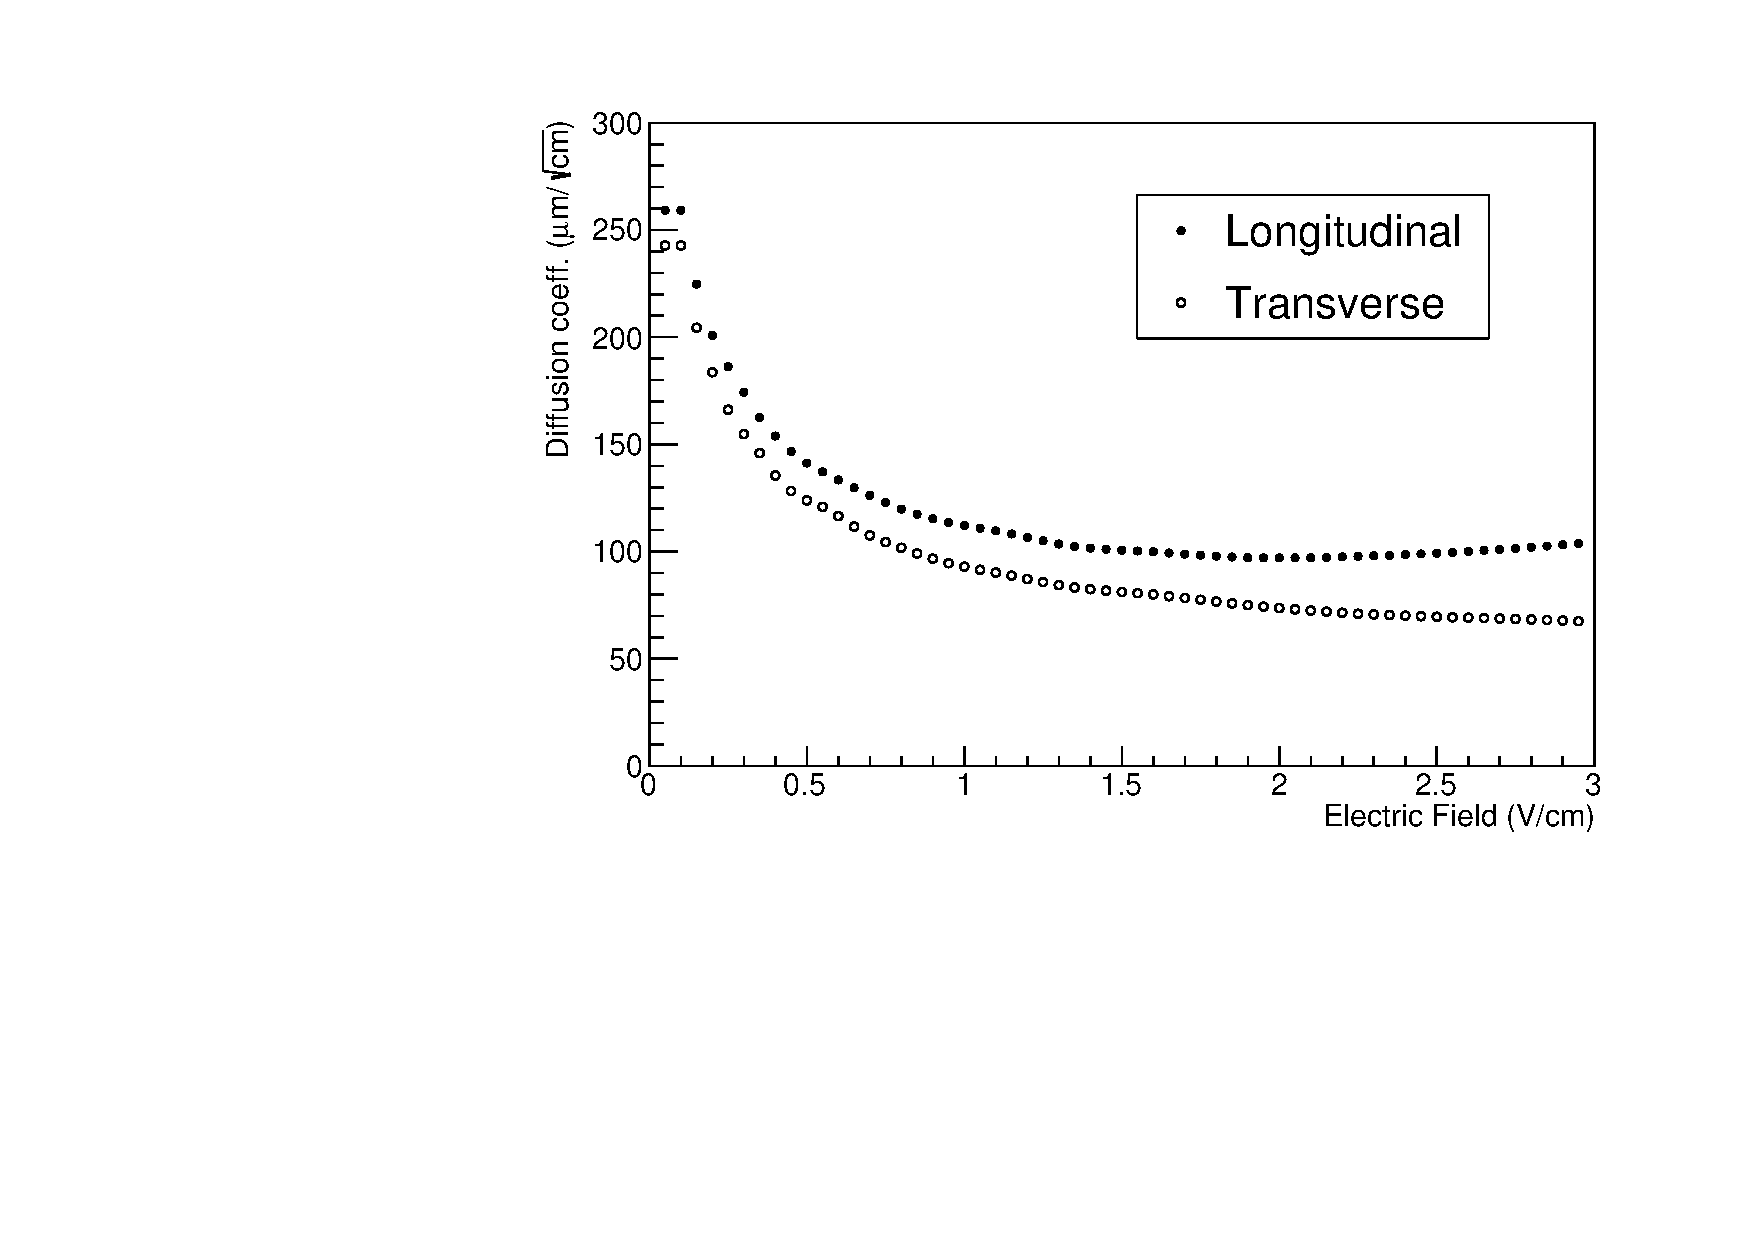
\includegraphics[width=0.35\textwidth]{diff6040_zoom.pdf}
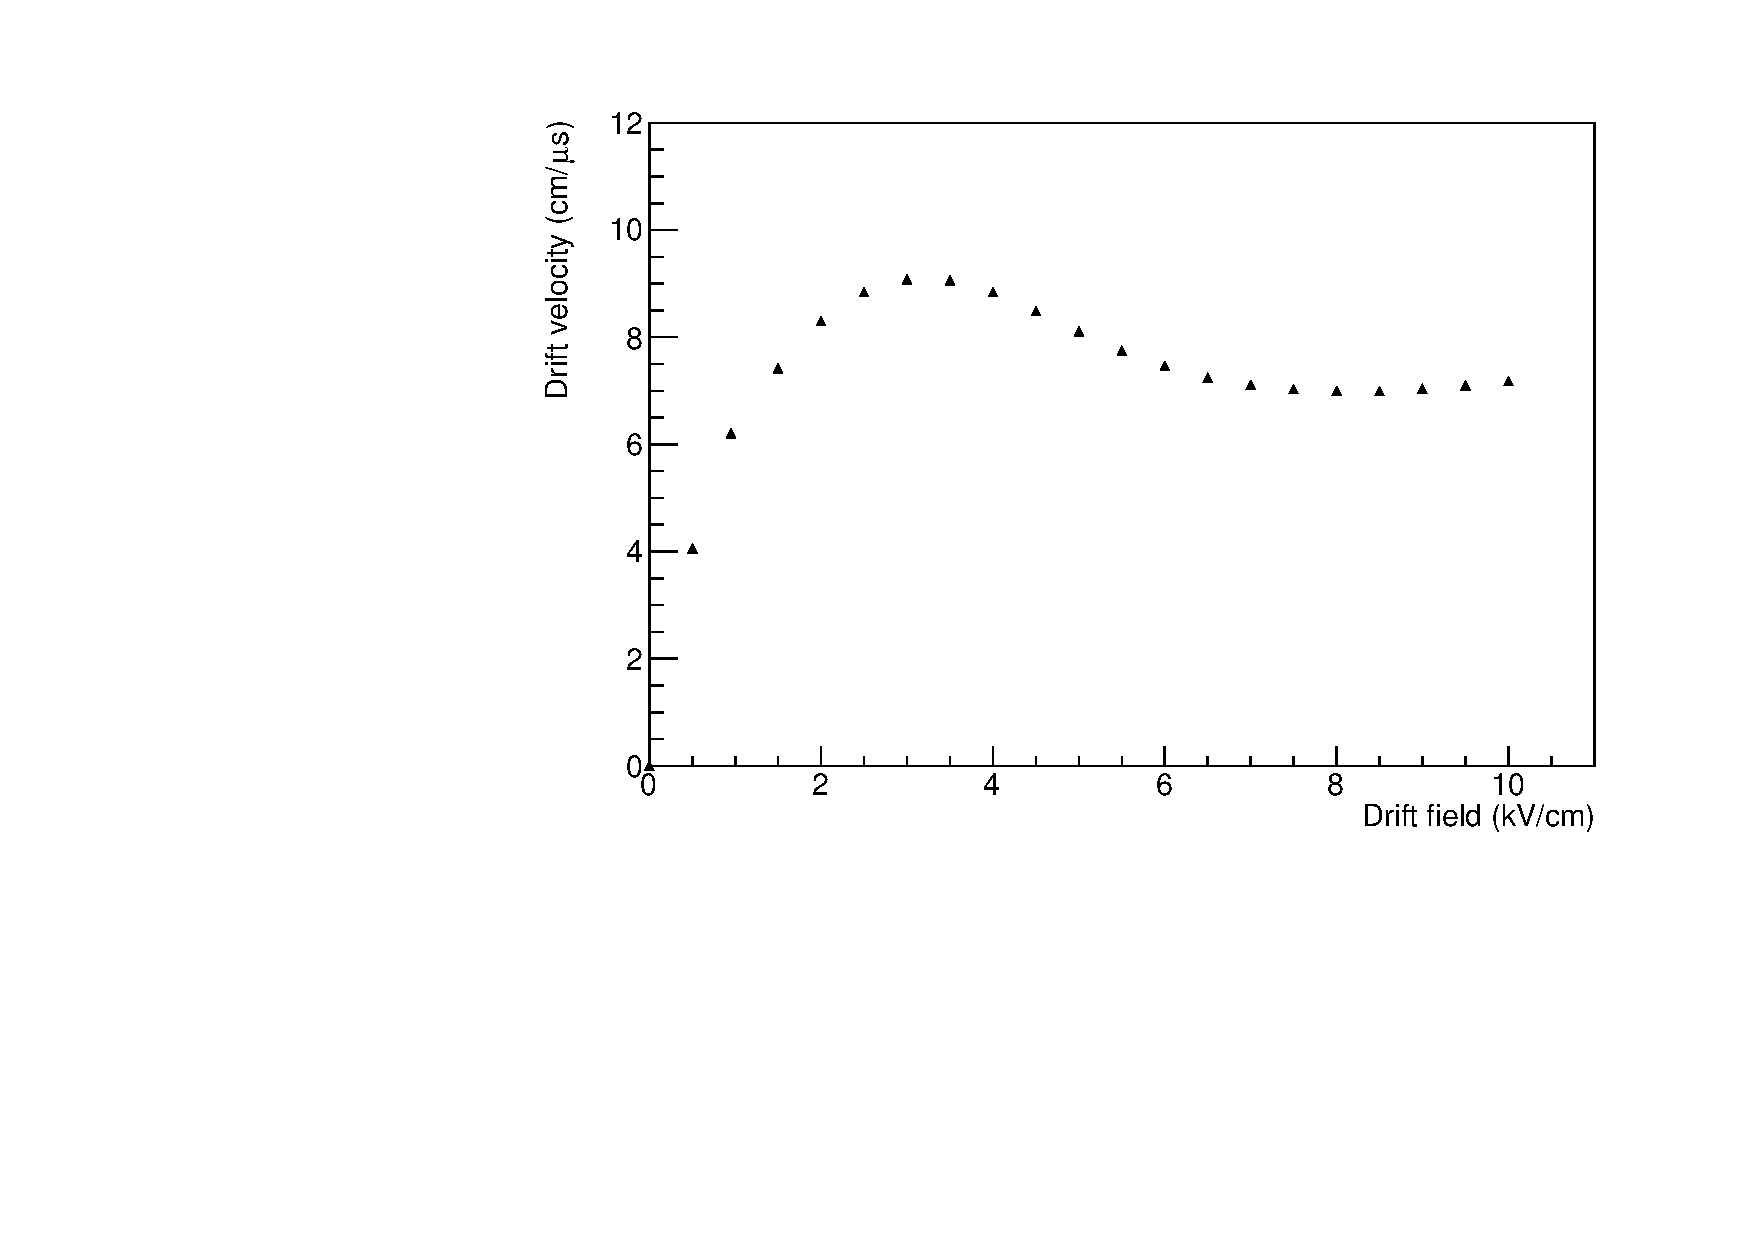
\includegraphics[width=0.35\textwidth]{vdrift6040.pdf}
%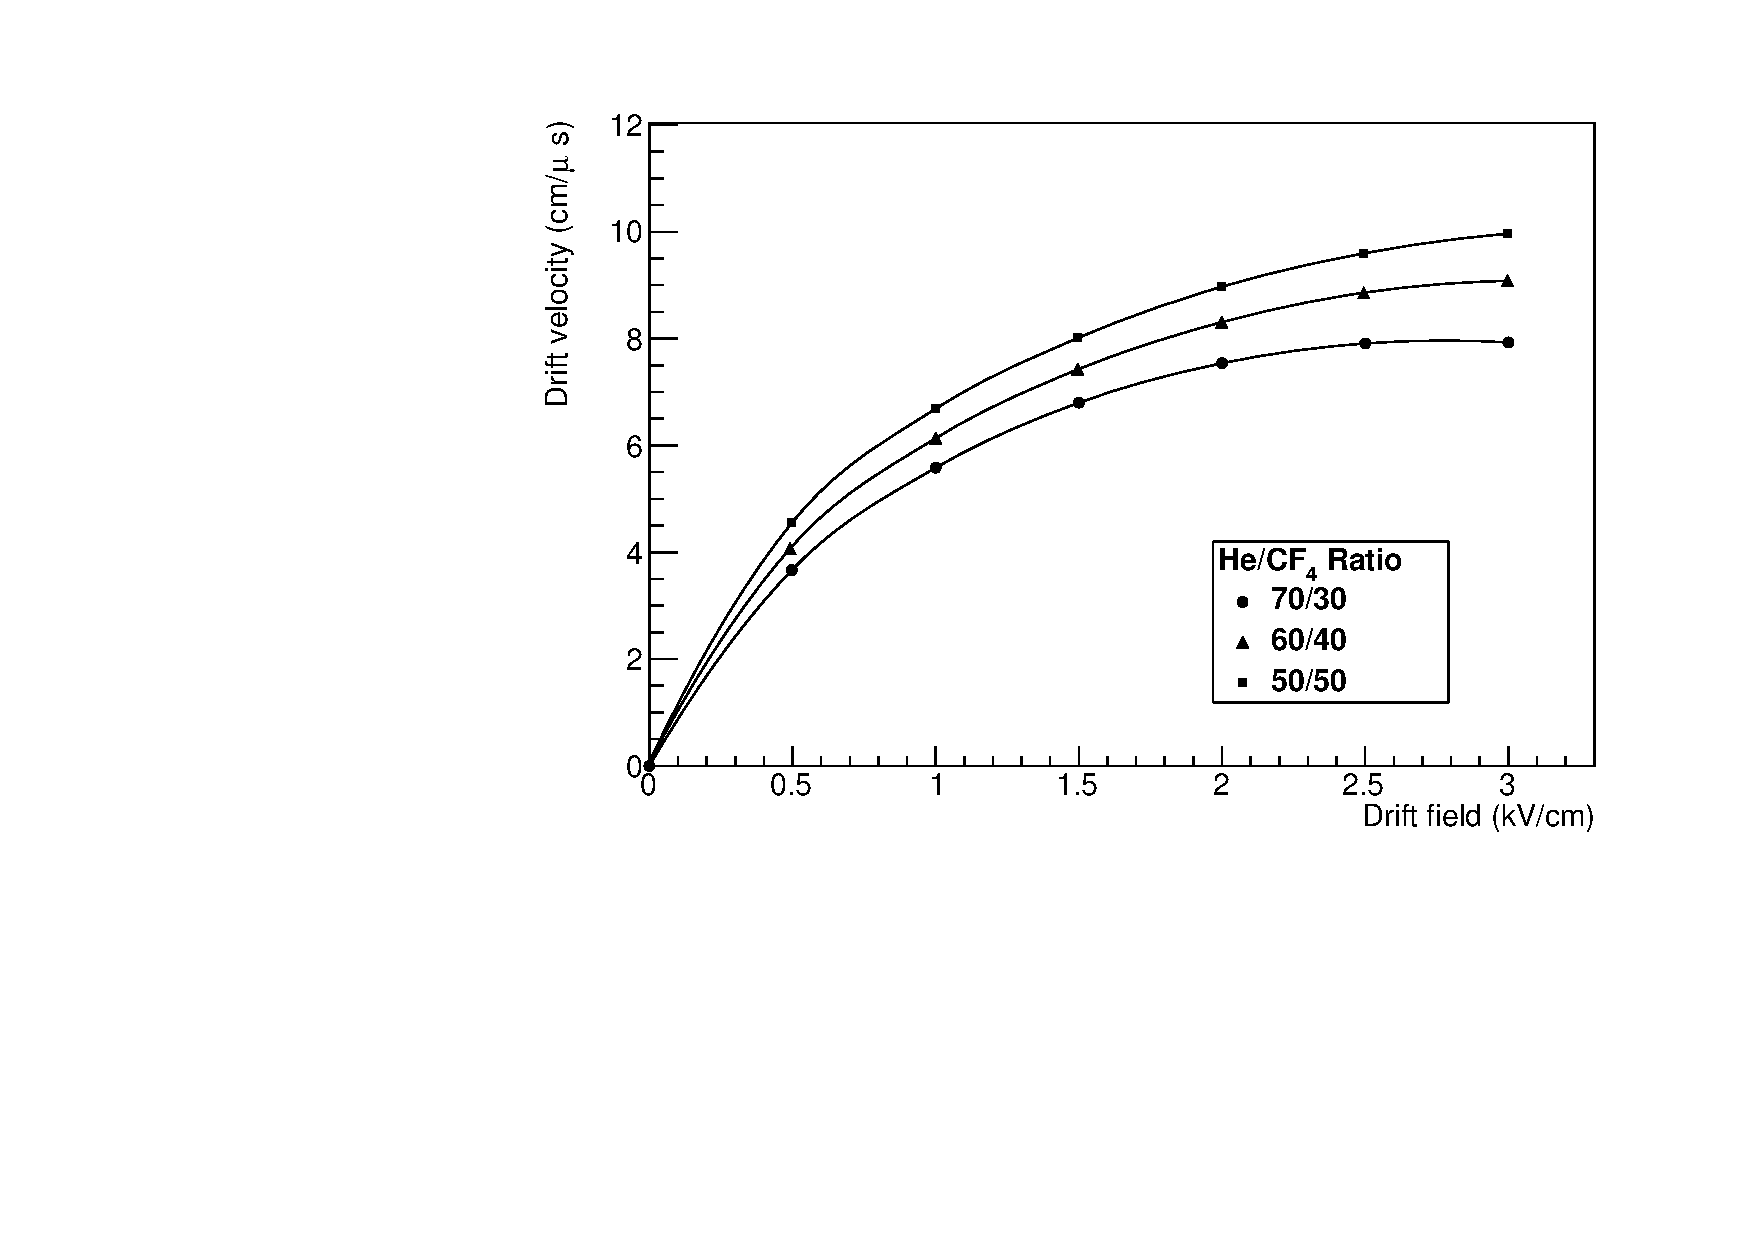
\includegraphics[width=0.35\textwidth]{vdrift.pdf}
\caption{Transverse and longitudinal diffusion coefficients for He/CF$_{4}$ 60/40 (left) and electron drift velocity (right) as a function of the drift field.}
\label{fig:diff_vdrift}
\end{figure}

% A gas mixture with a large fraction of a "cold gas" as the CF$_4$ have a small electron diffusion, and thus a small blur of initial signal shape, and quite high drift velocities for electric fields below 1 kV/cm. 

 
The effective ranges of electron and He-nuclei recoils were simulated
respectively with \GEANT~\cite{bib:geant} and
 \SRIM~software\footnote{Visit the {\it http://www.srim.org/} site for more information}. The average 3D ranges (i.e. the distance between production and absorption point) as a function of particle kinetic energy are shown in Fig.~\ref{fig:range}:
 \begin{itemize}
     \item He-nuclei recoils have a sub-millimetre range up to energies
       of 100\keV and are thus expected to produce bright spots with
       sizes mainly dominated by diffusion effects;
     \item low energy (less than 10\keV) electron recoils are in
       general larger then He-nuclei recoils with same energy and are
       expected produce less intense spot-like signals. For a kinetic
       energy of 10\keV, the electron range becomes longer than
       1\unit{mm} and for few tens of \keV, tracks of few centimetres
       are expected.
 \end{itemize}

\begin{figure}[t!]
  \begin{center}
    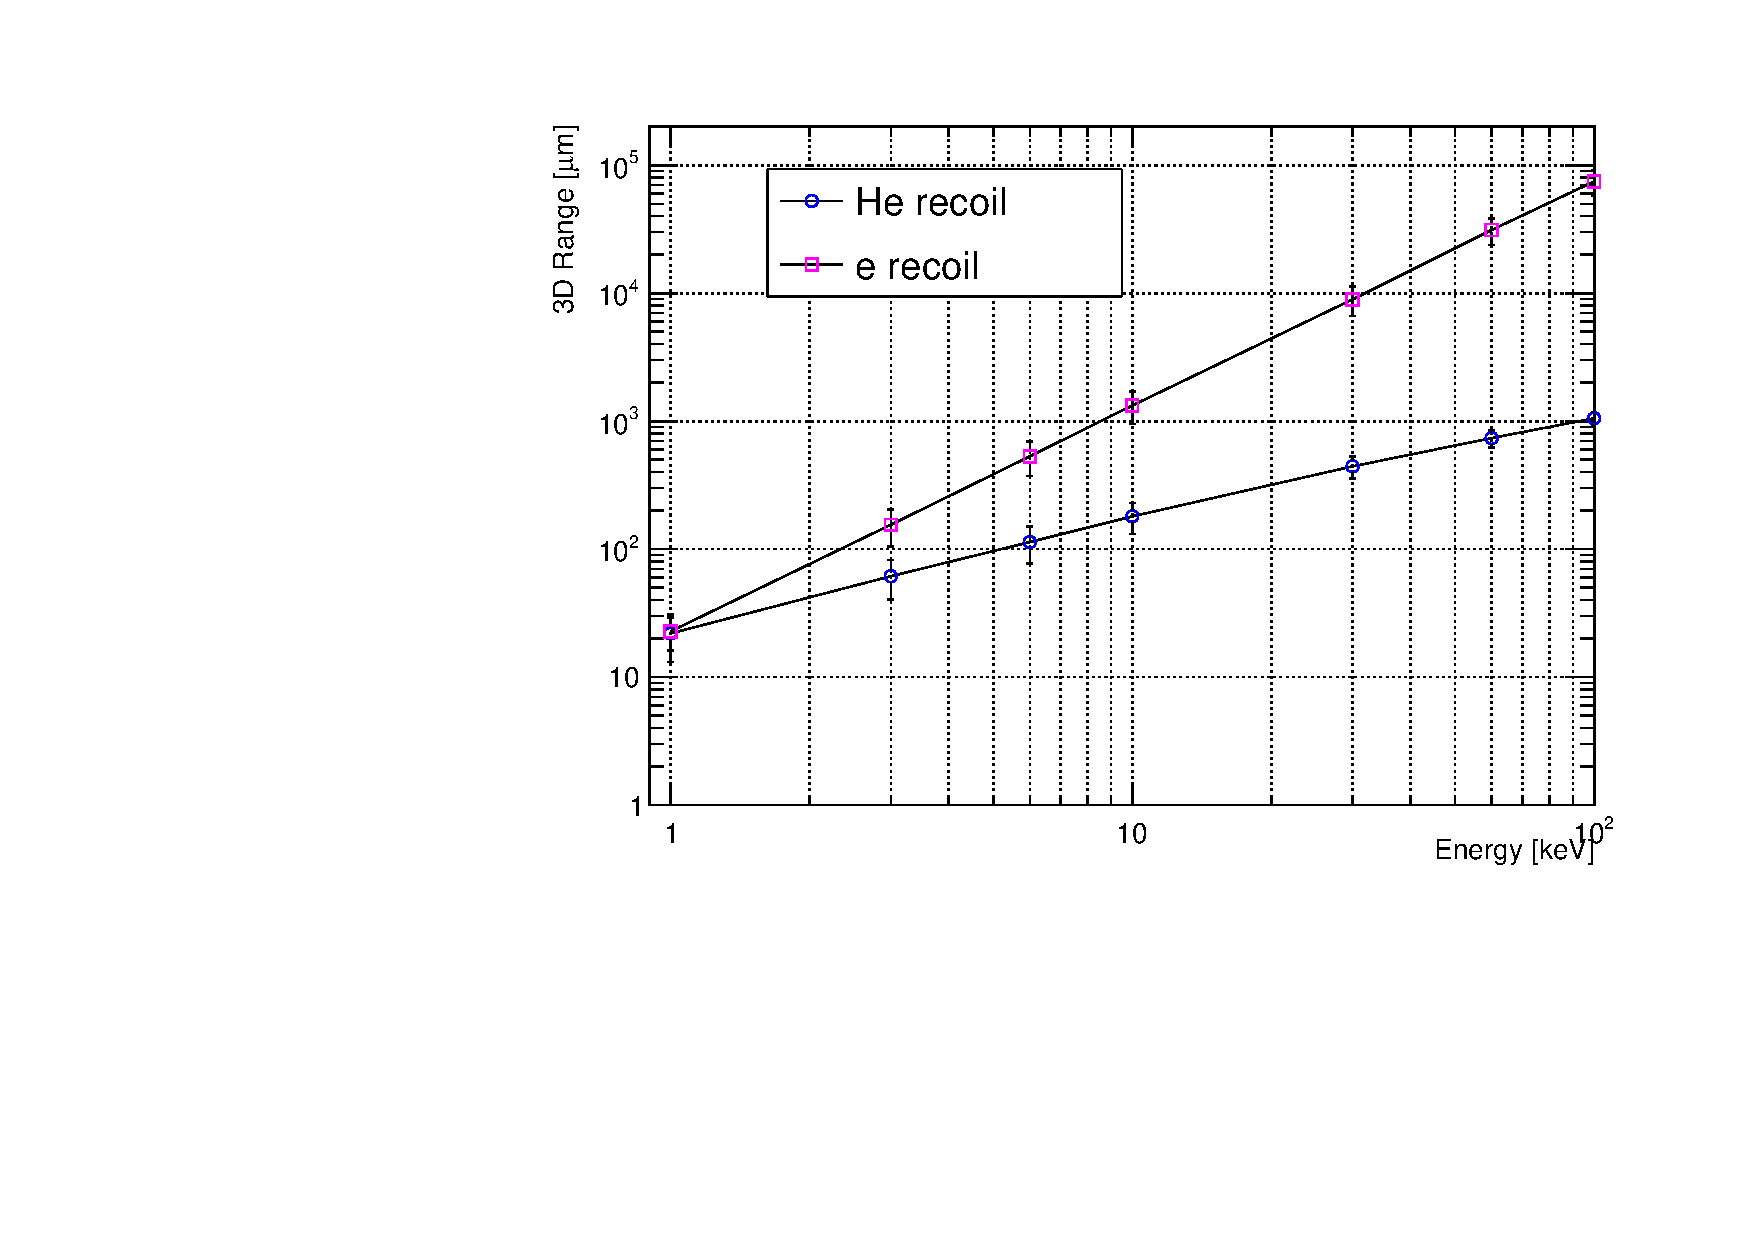
\includegraphics[width=0.49\linewidth]{range_ER_NR.pdf}
    \caption{Average 3D distance between production and absorption point for electron and He-nuclei recoils as a function of their kinetic energy.}
      \label{fig:range}
      \end{center}
\end{figure}







%\section{Experimental Results}
%\subsection{\lemon\ Prototype}
%All results reported in this paper were obtained with the Long Elliptical MOdule:~\lemon\
%shown in Fig.~\ref{fig:lemon}. 
%This detector, has following main characteristics:
%\begin{itemize}
%    \item a sensitive volume of 7 litres contained in a 20~cm long cylindrical field cage (FC) with an elliptical base with 24~cm and 20~cm axes;
%    \item a 24$\times$20~cm$^2$ triple-GEM stack closes the sensitive volume on  one side
%    \item mesh-based semitransparent cathode closes the volume on the other side
%\end{itemize}

%\begin{figure}[ht]
%\centering
%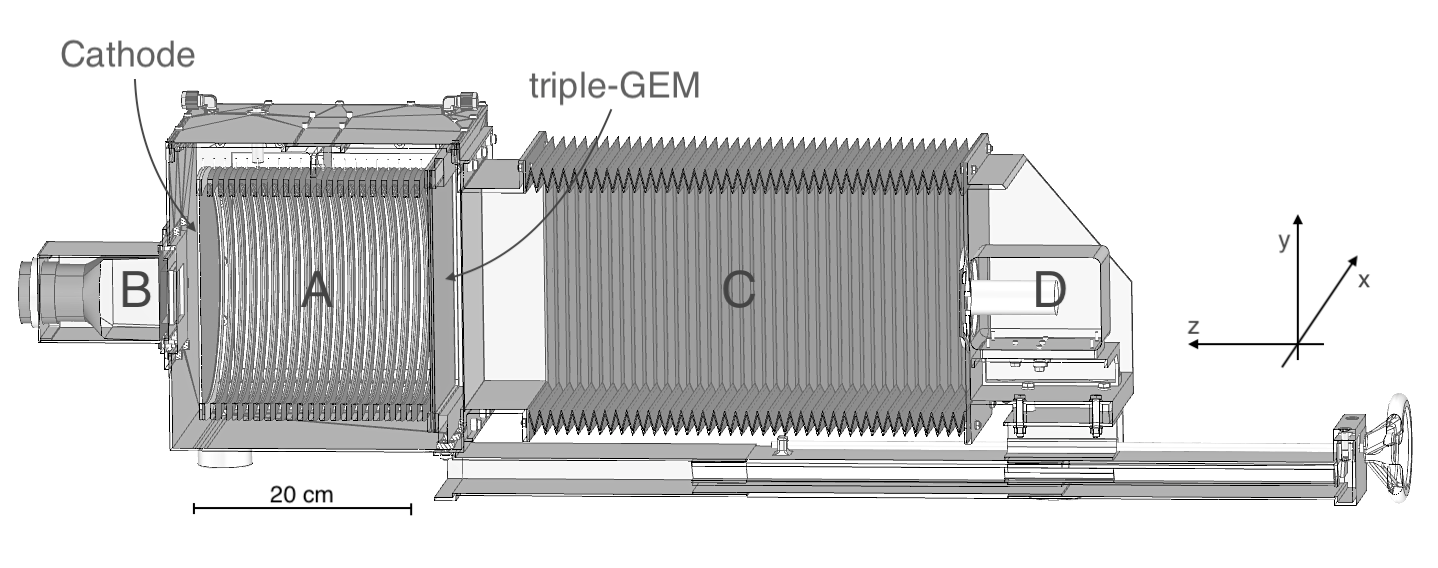
\includegraphics[width=0.65\textwidth]{Fig2-lemon.png}
%\caption{The \lemon\ prototype. The elliptical sensitive volume (A), the fast photo-multiplier (B), the optical bellow (C) and the sCMOS-based camera (D) are indicated.}  
%\label{fig:lemon}
%\end{figure}

%\subsection{Optical Sensors}

%The typical operating configuration for \lemon was based on following sets: 
%\begin{itemize}
%    \item a gas flux of 200 cc/min;
%    \item an electric field within the sensitive volume \Ed~=~0.5~kV/cm;
%    \item an electric field in the 2~mm wide gaps between the GEMs \Et~= 2.5~kV/cm;
%    \item a voltage difference across the two sides of each GEM \Vg~=~460~V;
%\end{itemize}

%According to results presented in \cite{bib:roby}, in this configuration an electron gain of about 1.5$\times 10^6$ is expected.

%\label{sect:sensors}
%\vspace{3mm}
%\subsubsection{{\bf sCMOS-based Cameras}}
%\vspace{2mm}

%As anticipated in Sect.\ref{sect:opro}, high quality cameras are a crucial ingredient for the experiment results. 
%Different cameras were tested during the R\&D phases~\cite{bib:cameras}. 
%All results shown in this paper were obtained by using 
% an ORCA Flash 4.0 camera\footnote{For more details visit www.hamamatsu.com}. This device in based on a 1.33~$\times$~1.33~cm$^2$ scientific CMOS sensor, subdivided in 2048~$\times$~2048 pixels with an active area of 6.5~$\times$~6.5~$\mu$m$^2$ each, with
 %a quantum efficiency of 70\% at 600~nm and a readout noise of 1.4~electrons.
 %The response and noise level of this sensor were tested with a calibrated light source \cite{bib:jinst_orange1}. A response of 0.9 counts/photon was measured together with a pedestal fluctuation of the pedestal of 1.3 photons/pixel. 
 
 %This sensor was usually equipped with a Schneider lens with 25~mm focal length $f$ and 0.95 aperture $a$. The lens was placed at the distance $d$ necessary to make the acquisition of the whole GEM surface possible. 

%\vspace{3mm}
%\subsubsection{{\bf Fast light-sensors}}
%\vspace{2mm}

%The main limitation of high granularity CMOS sensors is 
%represented by their poor timing information. The maximum possible readout rate of the order of 1 kHz would not allow to have a "time-stamping" better than 1 ms.

%In order to perform a 3D track reconstruction, the profile of the electron
%arrival times on the GEM should be acquired.

%To overcome this limitation, CYGNO developed the idea of combining the slow sCMOS camera with fast light sensors (PMT os SiPM).
%Performance of the combined light readout were tested with the use of a fast PMT \cite{bib:combined} and it was possible to evaluate a resolution on the reconstructed relative {\it z} coordinate of charge clusters of about 100 $\mu$m.

%The information provided by a fast light sensor will be exploited to reconstruct the signal time development and, therefore, its projection on the axis orthogonal to the GEM plane. Different PMT and SiPMT were tested during the R&D phase to individuate the most appropriate in terms of sensitivity and time resolution.

%Results presented here were obtained with a
%Photonics XP3392 Photo Multiplier Tube (PMT) with a 5~ns rise-time, a maximum QE for 420~nm and a 76~mm square-window.


\section{Experimental Results with CYGNO Experiment Prototype}\label{sec:results}
The experimental results obtained with the prototype named Long Elliptical MOdule:~\lemon\ represents the most comprehensive example currently available of the performance achievable with the CYGNO approach.
The ~\lemon\ detector,  shown in Fig.~\ref{fig:lemon}, is schematically composed by:
\begin{itemize}
    \item a gas sensitive volume of 7 litres contained in a 20~cm long cylindrical field cage (FC) with an elliptical base with 24~cm and 20~cm axes;
    \item a 24$\times$20~cm$^2$ stack of three GEM as the amplification stage facing the CMOS camera;
   \item a mesh-based semitransparent cathode closing the volume on the opposite side, behind which a PMT is placed;
\end{itemize}
A more detailed description of this prototype can be found in Ref.\cite{bib:fe55} and \cite{bib:lemon_btf}.

\begin{figure}[t!]
\centering
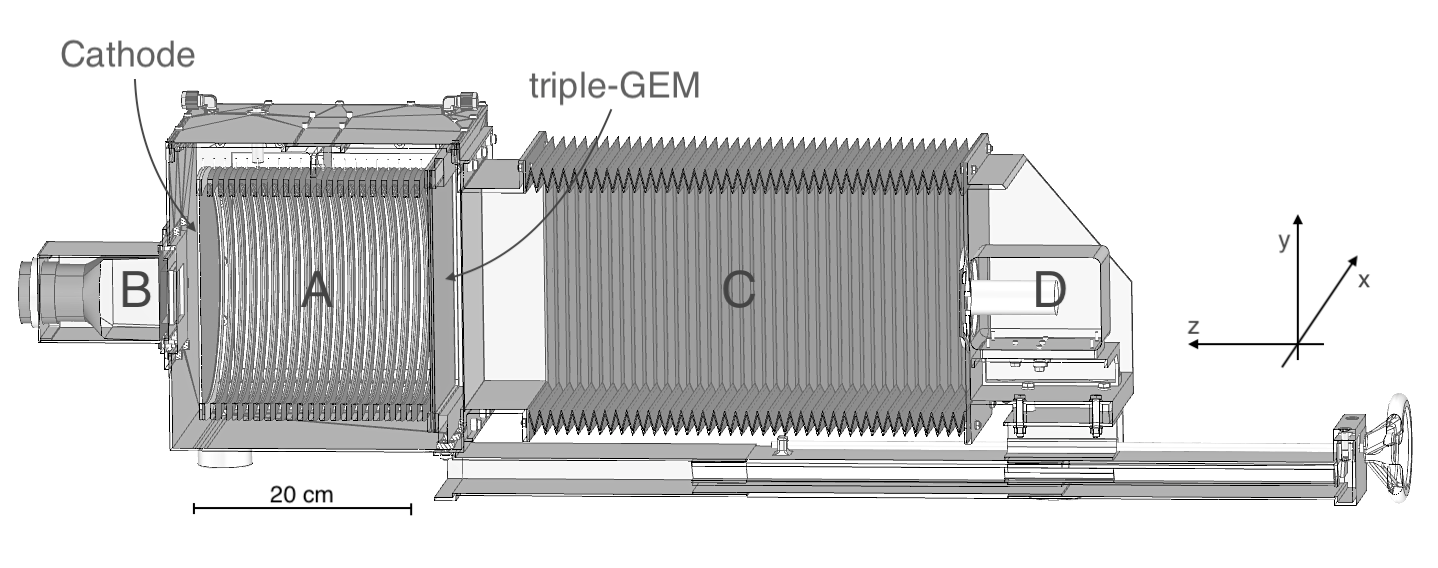
\includegraphics[width=0.65\textwidth]{Fig2-lemon.png}
\caption{The \lemon\ prototype \cite{bib:Antochi_2021}. The elliptical sensitive volume (A), the fast photo-multiplier (B), the optical bellow (C) and the sCMOS-based camera (D) are indicated.}  
\label{fig:lemon}
\end{figure}

\lemon\ standard operating conditions were based on following sets: 
\begin{itemize}
    \item an He/CF$_4$ (60/40) gas mixture flux of 200 cc/min;
    \item an electric drift field within the sensitive volume \Ed~=~0.5~kV/cm;
    \item an electric transfer field in the 2~mm gaps between the GEMs \Et~= 2.5~kV/cm;
    \item a voltage difference across the two sides of each GEM \Vg~=~460~V;
\end{itemize}

According to results presented in \cite{bib:roby}, in this configuration an electron multiplication of about 1.5$\times 10^6$ is expected.

%\subsection{{\bf sCMOS-based Cameras}}

As anticipated in Sect.~\ref{sect:opro}, high quality cameras are a crucial ingredient for the experiment results An ORCA Flash 4.0 camera\footnote{For more details visit www.hamamatsu.com} was selected to equip \lemon. This device in based on a 1.33~$\times$~1.33~cm$^2$ scientific CMOS sensor, subdivided in 2048~$\times$~2048 pixels with an active area of 6.5~$\times$~6.5~$\mu$m$^2$ each, with a quantum efficiency of 70\% at 600~nm and a readout noise of 1.4~electrons rms. The response and noise level of this sensor were tested with a calibrated light source \cite{bib:jinst_orange1}. A response of 0.9 counts/photon was measured together with a rms fluctuation of the pedestal of 1.3 photons/pixel. 
 
 %This sensor was usually equipped with a Schneider lens with 25~mm focal length $f$ and 0.95 aperture $a$. The lens was placed at the distance $d$ necessary to make the acquisition of the whole GEM surface possible. 
In order to image the large GEMs surface, the camera is equipped with a Schneider lens with 25.6~mm focal length $f$ and 0.95 aperture $a$. Since at a distance $d$ the lens provides a de-magnification of:
\begin{equation}
\label{eq:demagnification}
 \delta = \frac{f}{d-f} 
\end{equation}
the camera optical system is placed at $d$=52.6~cm distance from the GEMs, in order to image a 26$\times$26~cm$^2$ area. The solid angle covered by the sensor, which in turn determine the geometrical acceptance of photons is given by

$$
\label{eq:omega}
\Omega = \frac{1}{\left(4(1/\delta+1)\times f \right)^2}
$$
resulting in $1.57 \times 10^{-4}$ for the \lemon\ layout. This is the price the optical readout approach needs to pay in order to image large areas, and that clarifies why high electron gain gas mixtures are needed to reach low energy detection thresholds.


%A limitation of high granularity CMOS sensors is 
%represented by their poor timing information. The maximum possible readout rate of the order of 1 kHz would not allow to have a "time-stamping" better than 1 ms, therefore preventing 3D reconstruction for the short tracks expected in the experiment energy range of interest.



In order to complement the 2D track projection recorded by the CMOS with the track trajectory along the drift direction, the arrival time profile of the primary electrons could be extracted from the signal induced on the third GEM bottom electrode. Nonetheless, this is expected (and explicitly shown in \cite{bib:jinst_orange2}) to suffer from a considerably large 
noise (typically due to jitter on the high voltage
supply line), that could prevent signal detection at the low energies at play.

To overcome this limitation, light track time profile was concurrently readout by a Photonics XP3392 Photo Multiplier Tube (PMT) with a 5~ns rise-time, a maximum QE for 420~nm and a 76~mm square-window, providing sensitivity to single photon and significant reduced noise with respect to the GEM electric signal. 

%\subsection{Performance Studies}

Performance of \lemon\ were tested in recent years at Laboratori Nazionali di Frascati of INFN (LNF) overground laboratory by means of radioactive sources (\fe, \ambe), high energy (400 MeV) electrons from a beam at the BTF facility \cite{bib:btf1,bib:btf2} and cosmic rays, and are summarised in the following.

%\subsubsection{Operation Stability}
\subsection{Operation Stability}\label{sec:stability}

The performance and long term stability of \lemon\ was
tested for a month long run, during which the detector was exposed to environmental radioactivity, cosmic rays and a \fe~source~\cite{bib:fe55New}. During the whole period, all currents drawn by the high voltage channels supplying the electrodes of the GEM stack were monitored and recorded to identify sudden and large increases that could indicate discharges or other electrostatic issues.

During the test, two different kinds of electrostatic instabilities were observed:

\begin{itemize}
    \item hot-spots appearing on the GEM surface. While in some  cases these would fades out with time, sometimes they started to slowly grow up to tens of nA (on a time scale of minutes). These are very likely due to self-sustaining micro-discharges happening in one or few GEM channels. 
    
    \item high charge density due to very high ionizing particles or charge accumulation on electrode imperfections can suddenly discharge across GEM channels. In these events, a sudden increase in the drawn current is recorded with a voltage restoring on the electrodes through protection resistors on a few seconds time basis.  Even if these events are less frequent than hot spots, they can be dangerous for the GEM structure and the energy released in the discharge can, in principle, damage it. 
\end{itemize}

An automatic recovery procedure was implemented, triggered by the raising of the GEM currents, able to recover both hot-spots and discharges by lowering and gradually restoring the GEM voltages operating conditions in few minutes.

An average of 16 of such instabilities were observed per day and the total dead time introduced by the recovering procedures was less than 4$\%$. A detailed analysis of the time distance between two consecutive phenomena did not shown any correlation between two subsequent events, nor any increase of their rates. This allowed to conclude that detector operation looked very safe and stable and the obtained performance was completely satisfactory. Different gas proportion were tested and a lower amount of CF$_4$ resulted in a less stable electrostatic configuration. 

%Detector operational stability was evaluated during a month long test~\cite{bib:fe55New}. 
%During the whole period the behavior of all currents drawn by the high voltage channels supplying the electrodes of the GEM stack were monitored and recorded to identify sudden and large increases of drawn currents that can indicate discharges or other electrostatic issues.

%From the monitoring of detector current it resulted an occurrence probability of about 16 issues per day.
%A detailed analysis of the time distance between two consecutive phenomena didn't shown any correlation between two subsequent events neither any increase of their rates. This allowed to conclude that
%detector operation looked very safe and stable and the provided performance was completely satisfactory. 

%Moreover, the instability events gave rise to a detection inefficiency due to dead time introduced by recovering procedures of less than 4\%.

%Other gas proportion were tested and it resulted evident that a lower amount of CF$_4$, able to quench and avoid large charge productions gave a less stable electrostatic configuration. 

\subsection{Light Yield and Energy Resolution}\label{sec:yield}

The light production was evaluated by analysing CMOS and PMT response to interactions in gas of 5.9~keV X-rays produced by a \fe~source. The CMOS images were acquired in free running mode (i.e. without using any trigger signal) with an exposure of 100 ms. The CMOS pixels pedestal noise was extracted from the average of 100 images acquired in absence of any light signal and subtracted to each image before the analysis. An elementary clustering algorithm based on nearest neighbor-cluster (NNC) is applied to 4 $\times$ 4 rebinned images to select \fe\-like events.

Figure~\ref{fig:light} shows on the left the light spectrum of the \fe\ events reconstructed from the sCMOS images and on the right the integral of the charge signal measured by the PMT.

\begin{figure}[t!]
\centering
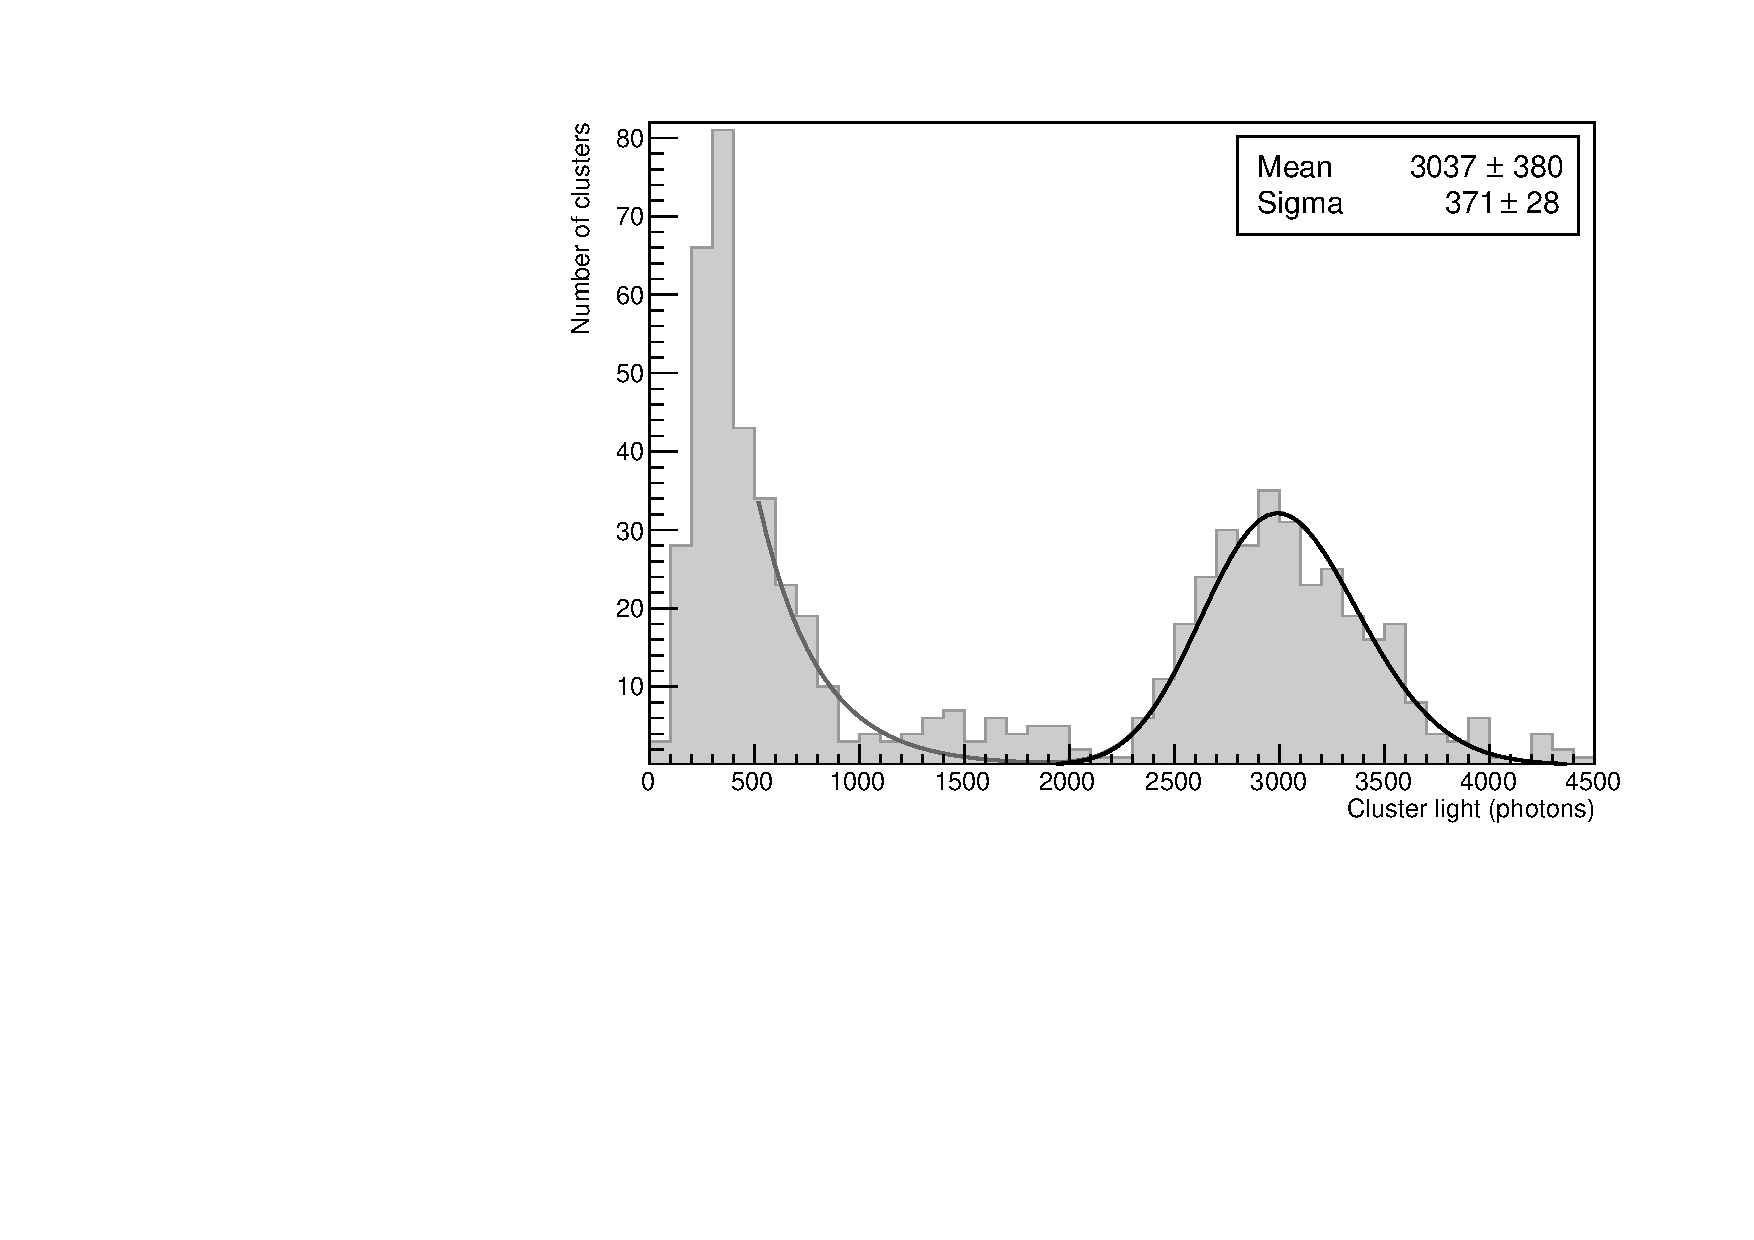
\includegraphics[width=0.35\textwidth]{DB_Integral_6040.pdf}
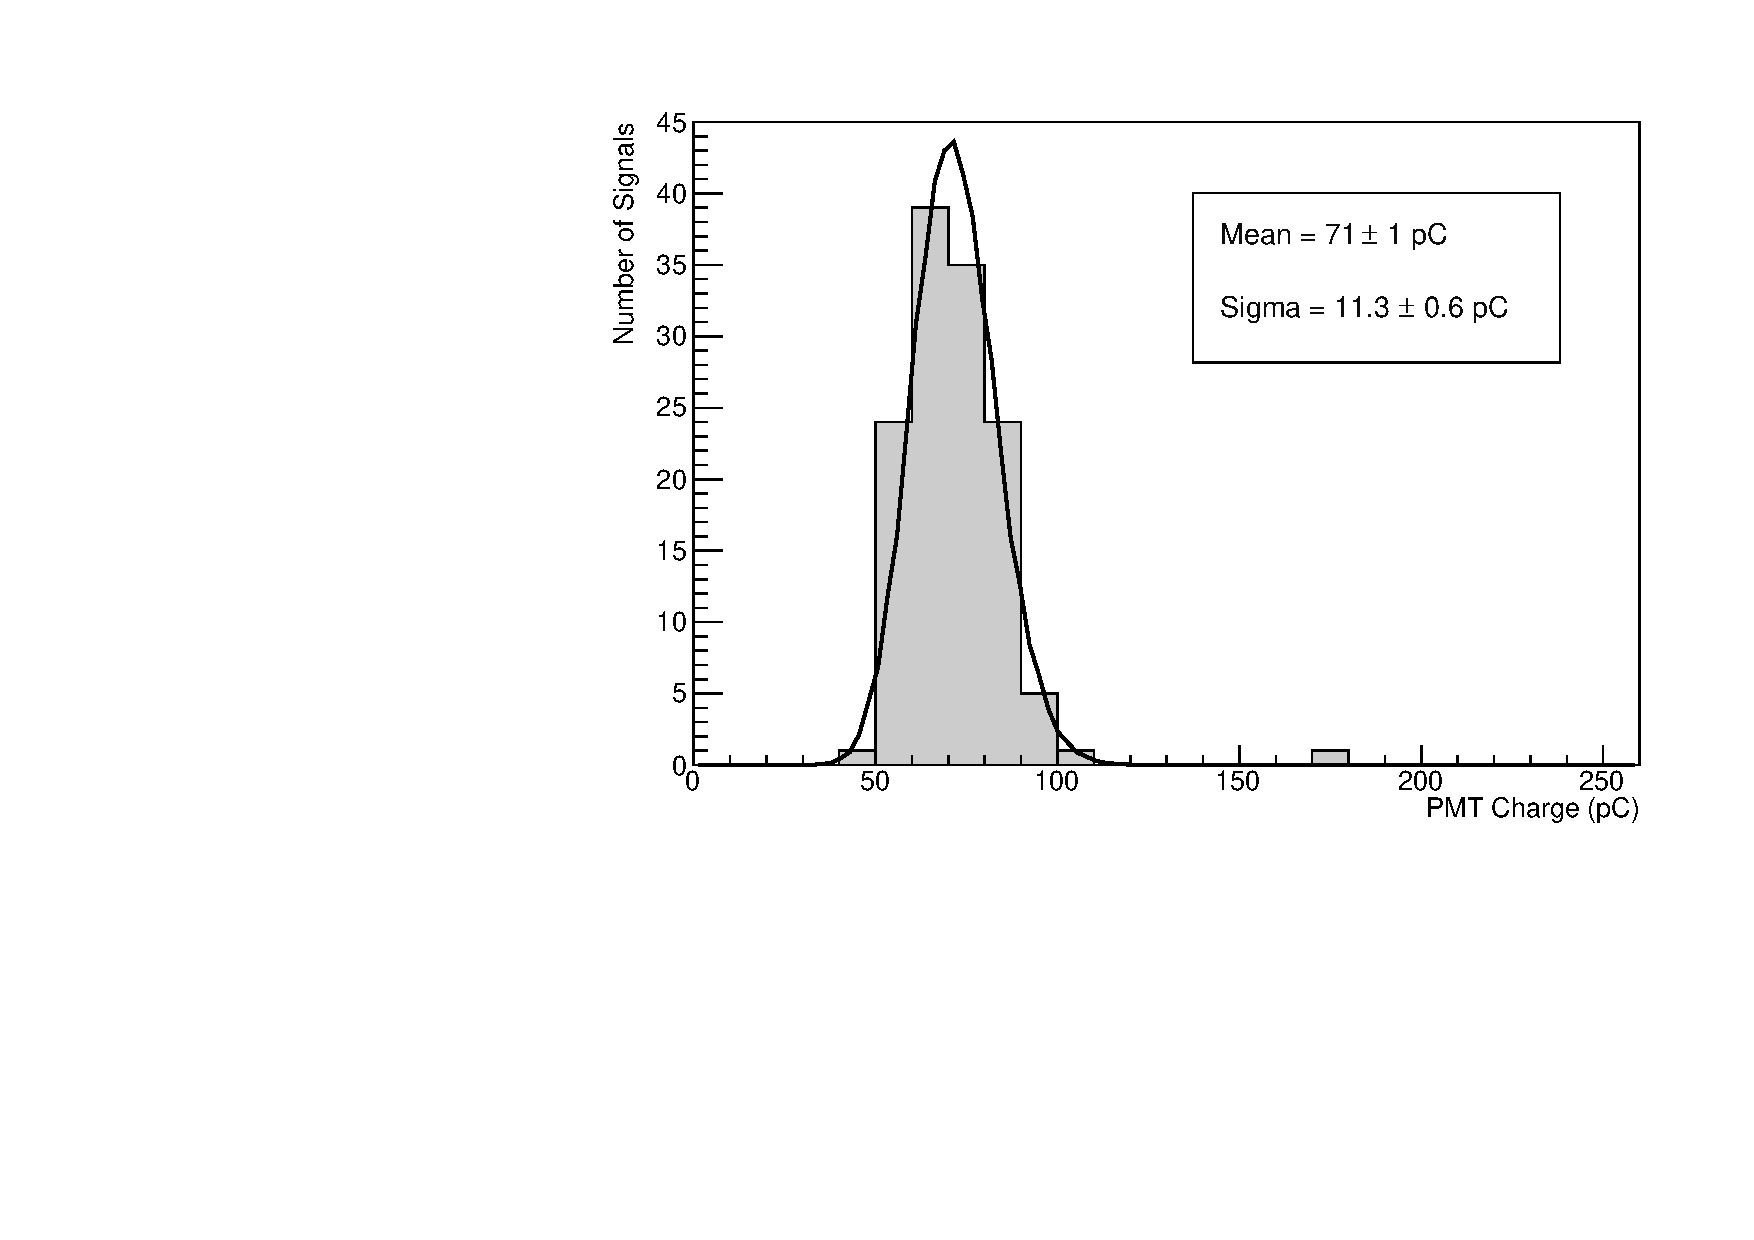
\includegraphics[width=0.35\textwidth]{newlightCharge_Run1834_Mix60-40.pdf}
\caption{Distribution of the light content of the \fe~events reconstructed from the sCMOS images  (left) and distribution of the charge measured by the PMT signals (right).} 
\label{fig:light}
\end{figure}

The average light yields were evaluated from a Polya fit \cite{bib:rolandiblum} to the two distributions, resulting in:
\begin{itemize}
    \item an average of 514~$\pm$~63 detected photons per keV released in the gas by the sCSMOS camera (in agreement with results obtained with lower \Vg\ and \Et\ \cite{bib:fe55}), with an energy resolution of 12\%;
    \item an average of (12.0~$\pm$~0.2) pC per keV released in the gas with an energy resolution of 16\% from the PMT charge signal;
\end{itemize}

\subsection{Detection Efficiency}

The detection efficiency along the whole 7~litres sensitive volume was studied acquiring CMOS images varying a collimated \fe\ source distance from the amplification plane and the electric drift field strength within the field cage Figure ~\ref{fig:deteff} shows on the left the number of reconstructed \fe\ spots in the CMOS images with the algorithm illustrated in Sec.\ref{sec:yield} as a function of drift field \Ed, normalized to the value obtained for \Ed~=~600~V/cm. For \Ed\ larger than 300~V/cm a plateau is found, indicating  a full detection efficiency for larger field values. Right panel of Fig.~\ref{fig:deteff} shows the dependence of $n$ on the source distance from the GEM amplification plane, normalised to its average value $\overline{n}$. A constant behavior is found in all tested positions, allowing to conclude that detection inefficiency is negligible down to 6 keV energy deposit.

\begin{figure}[t!]
\centering
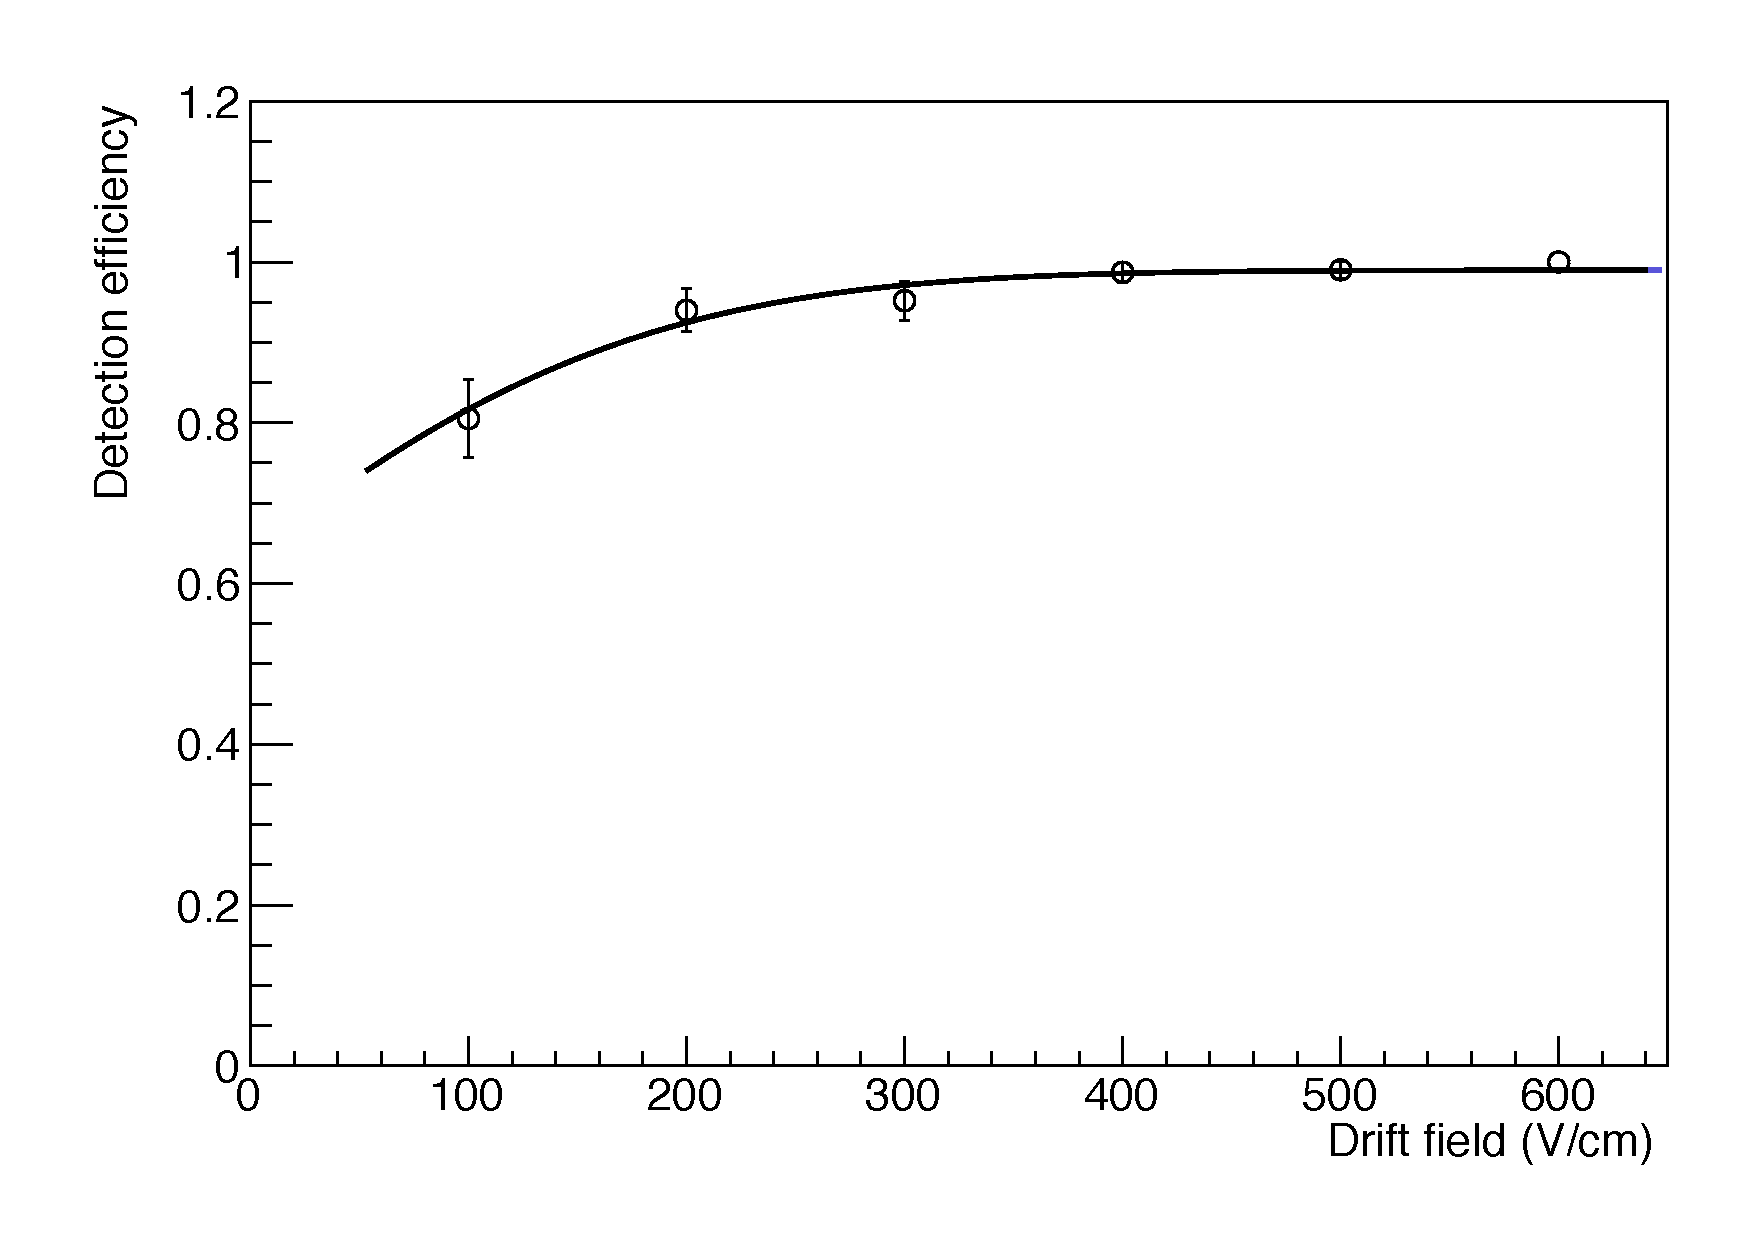
\includegraphics[width=0.35\textwidth]{gEff_Edrift.pdf}
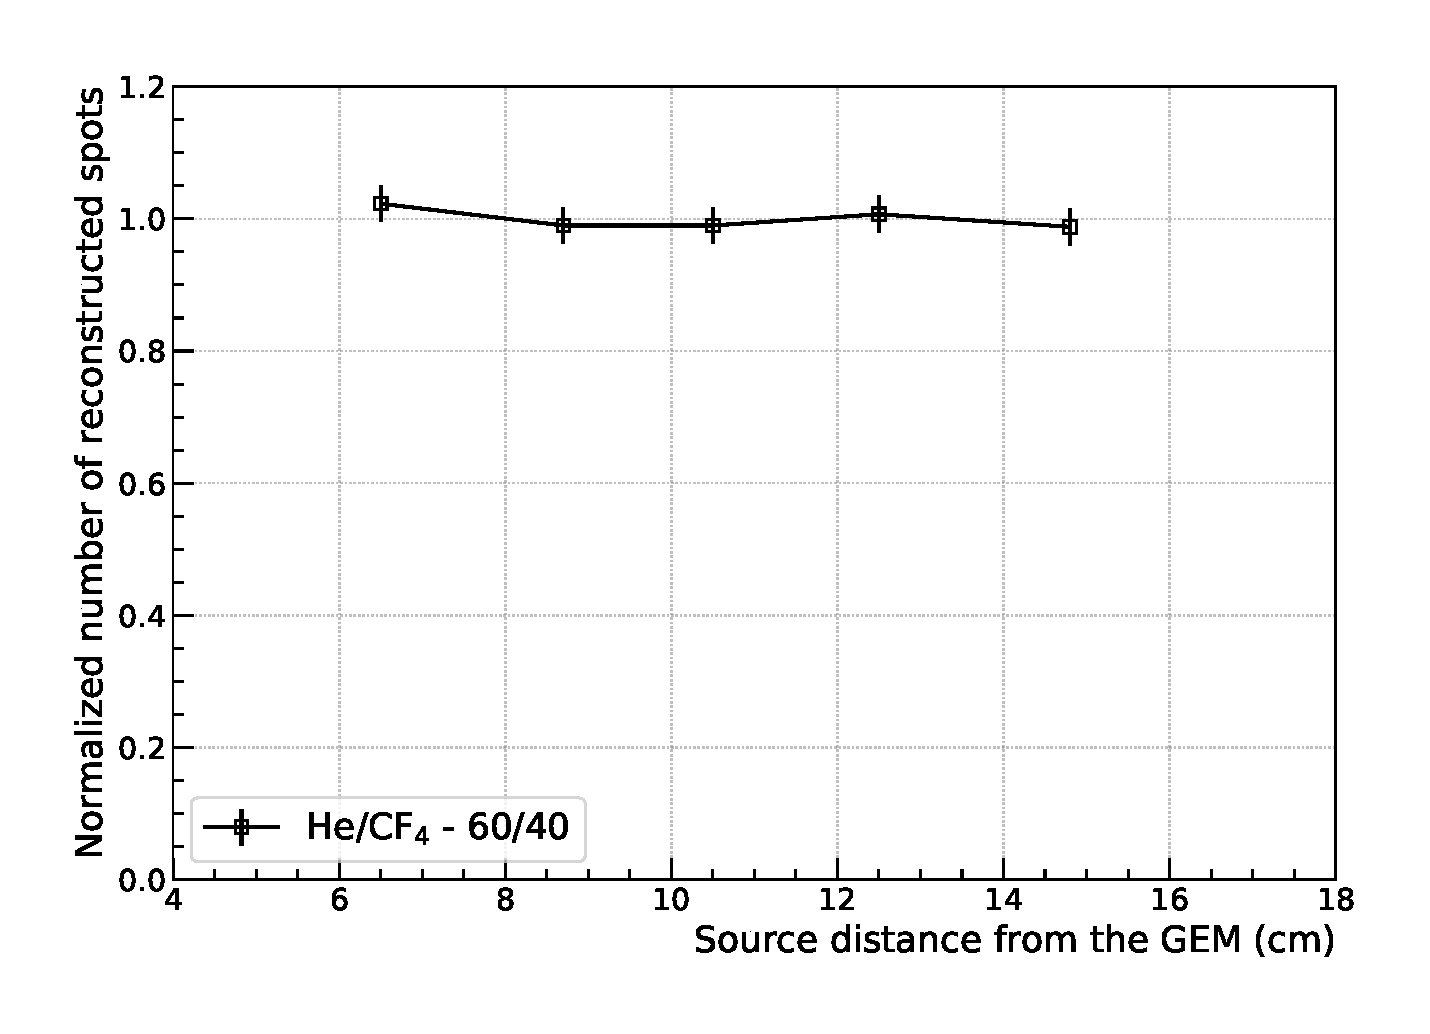
\includegraphics[width=0.35\textwidth]{feZscan6040_wo_4.pdf}
\caption{Behavior of the normalized number of \fe~spots as a function of drift electric field (left) and event depth in sensitive volume (right).} 
\label{fig:deteff}
\end{figure}


\subsection{Track absolute distance along the drift direction}\label{sec:track}
The possibility to determine the absolute $z$ position of the event in electron drift was studied with 450 MeV electrons from the LNF-BTF facility \cite{bib:lemon_btf}. The  transverse diffusion in the drift gap can in fact be exploited to extract the drift length and thus infer the absolute {\it z} distance at which the track occurred. 

Short 7~mm long track segments (having an average energy deposit of 1.5~\keV given the energy loss expected for 450 MeV electrons) were used to evaluate the detector performance for small energy releases. Figure~\ref{fig:eres} shows that a 40$\%$-50$\%$ energy resolution is achievable for such short segment (i.e. of the order of 1~\keV), with a position resolution between 100~$\mu$m (near the GEM plane) and 300~$\mu$m (20~cm~far from GEM plane).

\begin{figure}[t!]
\centering
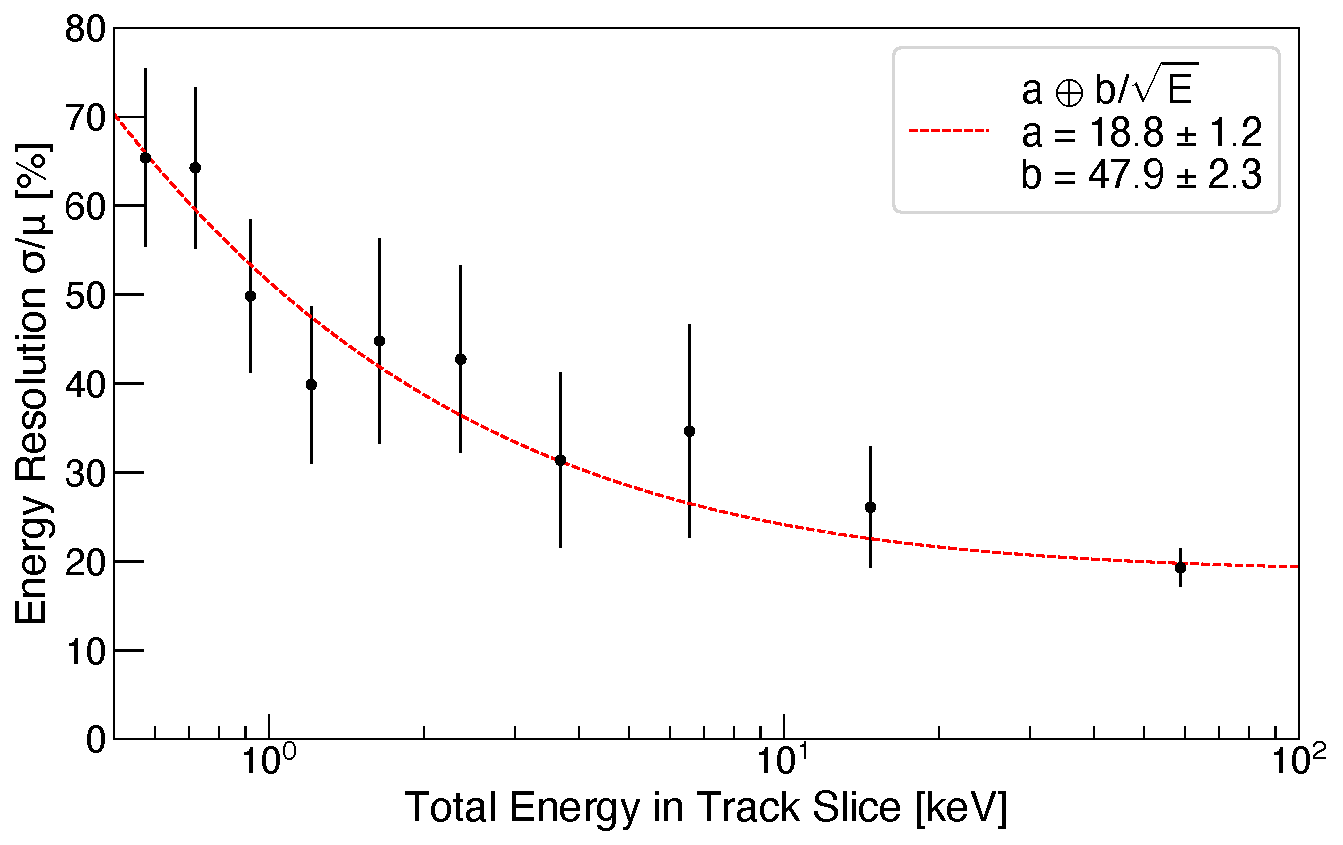
\includegraphics[width=0.40\textwidth]{EResBTF.pdf}
\caption{Behavior of the relative fluctuation of the energy measured in track segments of different length.} 
\label{fig:eres}
\end{figure}

As described in \cite{bib:Antochi_2021}, the light profile transverse to the track direction possesses a Gaussian shape with the total light being proportional to $\sigma_{light}$ $\times$ A$_{light}$ (where $\sigma_{light}$ is the sigma and A$_{light}$ the amplitude of the Gaussian). In the assumption of an electron absorption length $\lambda$ in the drift path and since diffusion increases as $\sqrt{z}$, the ratio $\eta_{light}$ = $\sigma_{light}$/A$_{light}$ is expected to grow quadratically with the drift distance~\cite{bib:lemon_btf}.

Similarly, longitudinal electron diffusion modifies the electron time of arrival on the GEM and thus the time structure of the signal recorded by the PMT. Also in this case, the ratio $\eta_{time} = \sigma_{time}/A_{time}$ between the amplitude and the width of the time waveform is expected to increase with {\it z}.


Figure \ref{fig:eta} shows the dependence of $\eta_{light}$ and $\eta_{time}$ as a function of {\it z} with a superimposed linear fit. 

\begin{figure}
\centering
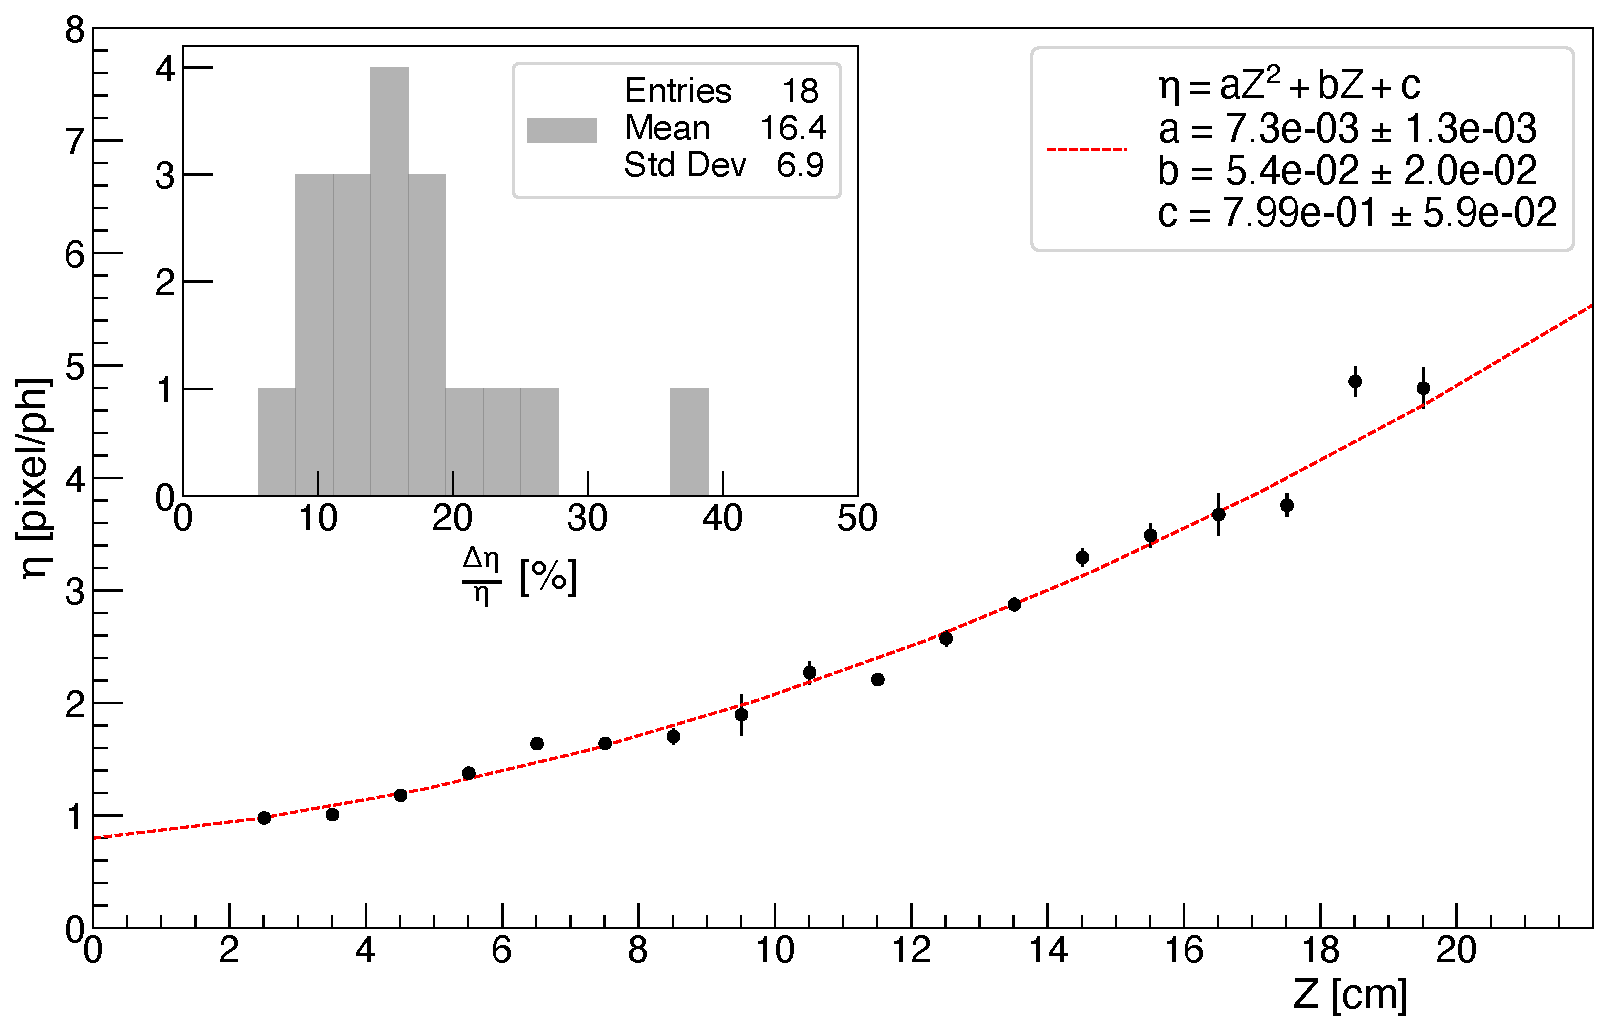
\includegraphics[width=.31\textwidth]{Fig9-eta-CMOS-Z.pdf}
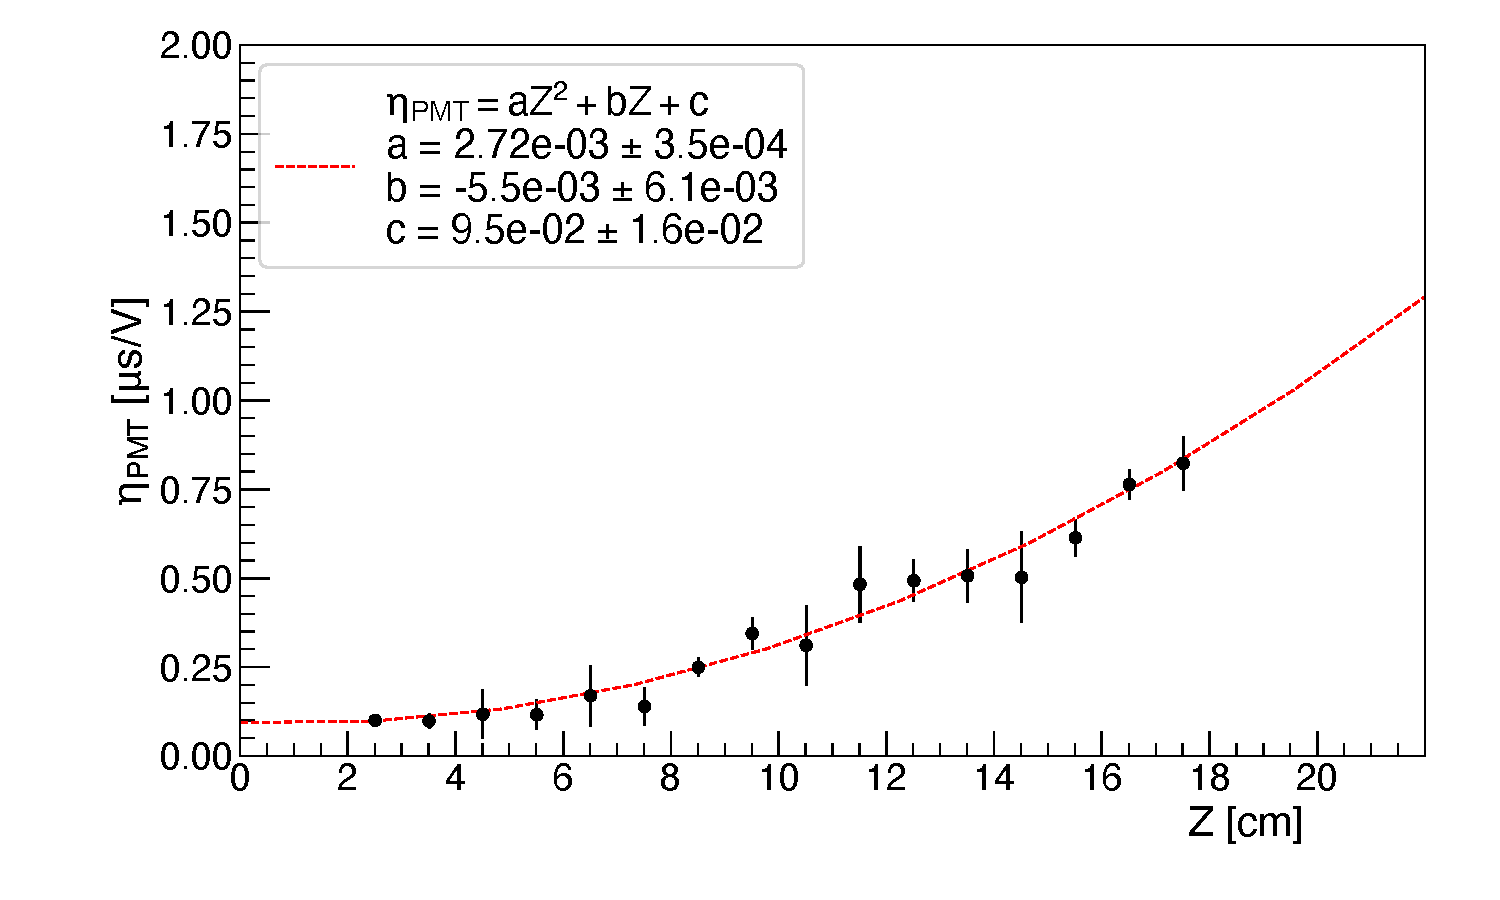
\includegraphics[width=.34\textwidth]{Fig10-eta-PMT-Z.pdf}
\caption{Dependence of $\eta_{light}$ on left and $\eta_{time}$ on the right as a function of the track distance from the GEM (see text for details).}
\label{fig:eta}
\end{figure}

These observables can be therefore used to evaluate the absolute $z$ with about 15$\%$ uncertainty over 20 cm length ~\cite{bib:lemon_btf}.

%The possibility to evaluate the track depth in the sensitive volume with precision of few centimetres is not typically available in TPCs lacking external triggers or the possibility of measuring the light produced by the interactions of the recoil itself with the gas ({\it primary light}).

These features result crucial in selecting the fiducial signal volume and therefore rejecting annoying backgrounds coming from radioactivity of TPC materials, like cathode or GEMs.






%\subsubsection{Tracking Performance}
%\label{sect:track}
%High energy particles crossing the detector can give rise to tracks several
%centimetres long.
%This can be the case for muons from cosmic rays of electron recoils with energies of about 100~keV or more. 
%Performance in reconstructing long tracks were studied at the Beam Test Facility (BTF) of "Laboratori Nazionali di Frascati" \cite{bib:btf1,bib:btf2}. The use penetrating minimum ionising particle allowed to make two different studies (described in details in \cite{bib:ieee17, bib:ieee18, bib:lemon_btf}), 

%On the one hand, the capabilities of finding and reconstructing long tracks in gas were tested. The energy resolution was measured as integrated along the particle trajectory. As shown in Fig.~\ref{fig:eres} for the whole tracks, an energy release of 40~keV was measured (in good agreement with an expected dE/dx of about 2.1~keV/cm evaluated for a $\simeq$~450 MeV electrons) with an energy resolution of about 20\%, similar to what was found with PMT measurements.

%On the other hand, short track segments were used to evaluate the detector performance for small energy releases. From simulation, three primary ionization e$^-$ clusters, for a total of five-six primary electrons, are expected per track millimeter. Figure~\ref{fig:eres} shows that for segments containing an energy of few hundreds of \eV is already possible to obtain an energy resolution of 40\%-50\% (i.e. of the order of 100~\eV).

%The 2D position on the plane parallel to the GEM's, of track segments with lengths of 7~mm (about 1.5~\keV) can be reconstructed with a resolution on relative position between 100~$\mu$m (near the GEM plane) and 300~$\mu$m (20~cm~far from GEM plane).
%Moreover, by exploiting the diffusion effect in gas, the third coordinate, (i.e. distance of each of those segments from the GEM) can be evaluated, separately by the CMOS sensor and PMT, with a precision between 10\% and 20\%.

\subsection{Detection and Identification of Nuclear and Electron Recoils}
\label{sect:rej}

Thanks to the detailed information provided by the high granularity optical sensors, track properties like shape, size, light density and so on can efficiently be exploited to identify and separate Nuclear Recoils (NR) expected from a DM signal from Electron Recoils (ER) coming from background sources.

To quantify these feature within CYGNO experimental approach, a track reconstruction and identification algorithm was developed for the analysis of the sCMOS images, called iDBSCAN \cite{Baracchini:2020iwg} and based on an adapted version of the well-known Density-Based Spatial Clustering of Applications with Noise (DBSCAN) \cite{dbscan1996}. The iDBSCAN, exploiting the number of photons in each pixel as a third dimension to the phase space of the points considered, separately identifies clusters displaying different intensity (i.e. energy deposition patterns), and therefore likely belonging to different classes of particles interactions.

The performance of the algorithm were studied on 5.9 keV energy deposit from $^{55}$Fe and NR  produced by an \ambe~source \cite{bib:coronello}. The 59 keV$_{ee}$ photons produced by \ambe~were nearly completely shielded by a lead shield built around the detector. Data were taken overground at LNF and were therefore highly contaminated by cosmic ray particle interactions.


In order to  select a pure sample of nuclear recoil candidates produced by the interaction of the neutrons
originating from the source and to identify various sources of backgrounds, several cluster shapes observables were exploited. Among these, the \emph{slimness} ($\xi$) was used to mainly distinguish cosmic rays  and the light \emph{density} ($\delta$) to discriminate electron from nuclear recoils. The slimness is the ratio of the Gaussian width of the track in the transverse direction over the projected path length. The density is the ratio of the total number of photons detected by all the pixels gathered in the cluster over the total number of pixels. 

Exploiting a simple selection on $\delta$,  an ER background rejection in the energy region around 5.9 keV$_{ee}$ of 96.5$\%$ (99.2$\%$) was found together with  50$\%$ (40$\%$) NR efficiency ~\cite{bib:coronello}.


%Low energy photons produced by natural radioactivity can ionize electrons from atoms and molecules in the detector, producing recoils (ER) that would produce a signal similar to the ones produced by Dark Matter interactions, representing an important and dangerous background.

%Those ER deposit energy and interact with matter in a slightly different way with respect to NR. These differences can result in distinctive and diverse patterns of ionization charge and therefore different images. 

%Because of their larger mass and electric charge, nuclear recoils are
%expected to release their energy by ionizing the gas molecules in a few
%hundred \unit{$\mu$m} 
%while the electrons are able to travel longer
%paths.

%Given the detailed information provided by the high granularity optical sensors, it is possible to develop algorithms able to reconstruct not only the total deposited energy but also to identify and separate NR form ER down to few \keV kinetic energies
%based on the study of the properties of the images (shape, size, light density).

%To study and develop this possibility, CYGNO collaboration performed extensive studies by exposing 
%different prototypes to radioactive sources producing neutral particles.
%In particular, \lemon\ prototype was exposed
%to two kinds of neutral particles in an
%overground location:
%\begin{itemize}
%\item photons with energy of 5.9~\keV 
%  provided by a radioactive source of \fe 
%  able to produce electron recoils with equal energy by means %of
%  photoelectric effect;
%\item neutrons with kinetic energy of few MeV produced by an %\ambe
%  source that can create nuclear recoils with kinetic energy lower
%  than the neutron ones.
%\end{itemize}


%The system demonstrated a capability of identifying 5.9\keV electron recoils
%with an efficiency of 96.5\% (99.2\%) against nuclear recoils by
%retaining a capability of detecting them with an efficiency of 50\%
%(40\%), averaged across the measured \ambe\ spectrum ~\cite{bib:coronello}
%as shown in Fig.~\ref{fig:coronello}.

 
% \begin{tabular}{ c  c  }
%\begin{minipage}[b]{0.39\textwidth}
%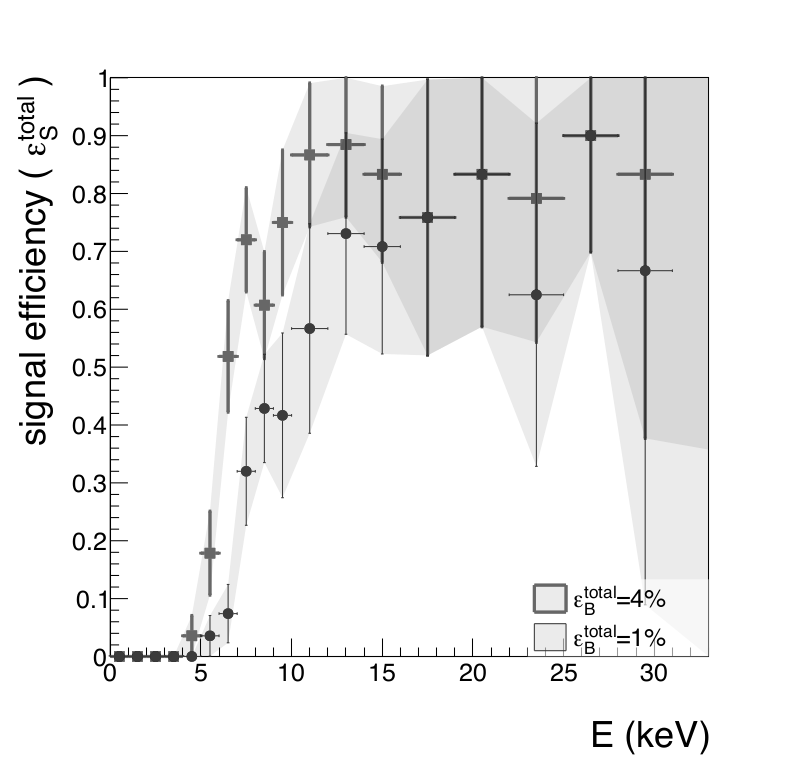
\includegraphics[width=\linewidth]{energyFull_effi_bw.png}
%    \captionof{figure}{Detection efficiency for nuclear recoils as a function of their energy %in the cases of electron recoils rejection of 96\% (squares) and 99\% (circles).}
%\end{minipage}
%
%  \begin{minipage}[b]{0.24\textwidth}
%
%    \begin{tabular}{l c | c }
%  \hline\hline
%  Working & Sig     & Bkg \\
%  Point   & eff     & rej \\
%\hline
% &  $\varepsilon_{S}^{total}$ &  $ R_{B}^{total}$ \\
%  \hline
%  $\mathrm{WP}_{50}$  & 0.50                     & 29 \\
%  $\mathrm{WP}_{40}$  & 0.40                     & 125 \\
%  \hline\hline
%\end{tabular}
%\captionof{table}{Signal and background efficiency for
%         two different selections sets.\label{tab:roc}}
%\end{minipage}
%\end{tabular}
 
\begin{figure}[t!]
  \centering
    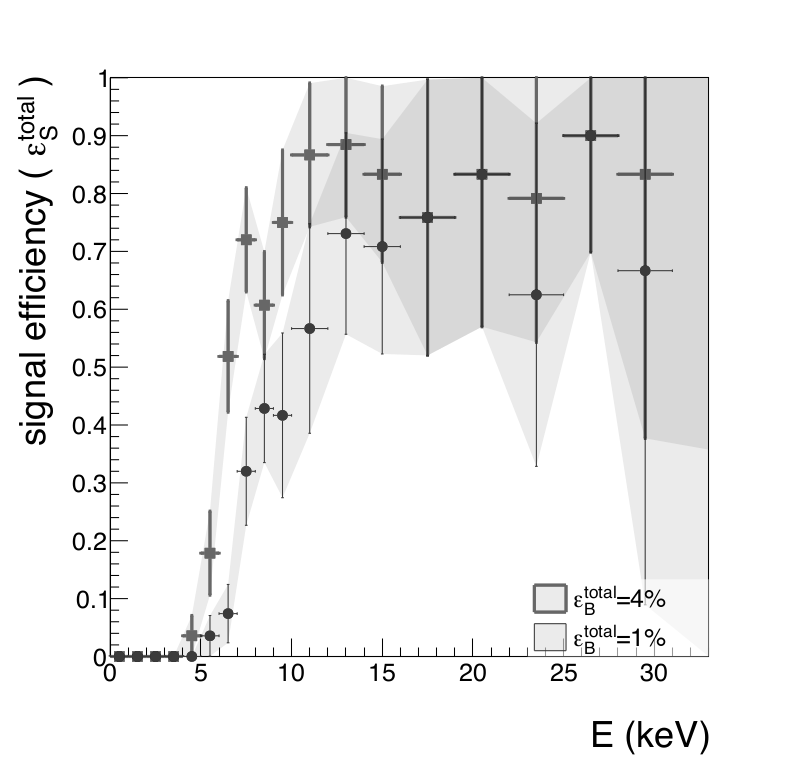
\includegraphics[width=0.49\linewidth]{energyFull_effi_bw.png}
    \caption{Detection efficiency for nuclear recoils as a function of their detected energy for electron recoils rejection of 96\% (squares) and 99\% (circles).}
      \label{fig:coronello}
\end{figure}

%\begin{table}[h!]
%\centering
%\caption{Signal (nuclear-recoil-induced by \ambe radioactive source) and background %(photo-electron recoils of X-rays
%         with $E=5.9$\keV from \fe radioactive source) efficiency for
%         two different selections sets.\label{tab:roc}}
%
%\vspace{10pt}
%\normalsize
%\centering
%\begin{tabular}{l c | c }
%  \hline\hline
%  working & Signal     & Background \\
%  point   & efficiency & rejection \\
%\hline
% &  $\varepsilon_{S}^{total}$ &  $ R_{B}^{total}$ \\
%  \hline
%  $\mathrm{WP}_{50}$  & 0.50                     & 29 \\
%  $\mathrm{WP}_{40}$  & 0.40                     & 125 \\
%  \hline\hline
%\end{tabular}
%\end{table}


%In particular, the nuclear recoil detection efficiency was measured to
%be 40\% for deposited energies lower than 20\keV and 14\% in the range
%(5--10)\keV.

%The electrons rejection factor (RF) 
%was evaluated for two example working points, $\mathrm{WP}_{40}$
%and $\mathrm{WP}_{50}$, having 40\% and 50\% signal efficiency. 
%The values obtained are respectively $\mathrm{RF}_{50}~=~29$
%and $\mathrm{RF}_{40}~=~125$.

%{ \red FORSE A LHC SI, ma nella DM RF non ha senso}


While this cut-based
approach is minimalist, and could be improved by more sophisticated analyses combining several topological variables and also the information from PMT waveforms, it shows
that a rejection factor larger than 10$^2$ for electron recoils at $E=5.9\keV$ can be obtained with a
gas detector at atmospheric pressure, while
retaining a high fraction of NR event signals.


%\section{The CYGNO Apparatus}
%CYGNO collaboration is working at the design for the final demonstrator to be installed underground at Gran Sasso National Laboratories (LNGS): CYGNO-1 with a sensitive volume of 1 m$^3$ based on the experience gained with previous prototypes.

%\section{Detector Description}\label{sec:detector}

%Sensitive gas will be contained in a box made of low radioactive PMMA material. The box will be, in both cases, 1 meter long with a cathode in the center to create two 50~cm drift regions.
%The electrons multiplication structure will be based on a stack of 3 standard 35$\times$35~cm$^2$ thin GEM's separated by 2~mm transfer gaps. Each stack will be readout with the latest generation sCMOS-based ORCA-Fusion Digital Camera\footnote{https://www.hamamatsu.com/eu/en/product/type/C14440-20UP/index.html} featuring 2304~$times$~2304 pixels with dimensions of $6.5~\times~6.5~\mu$m$^2$, providing a quantum efficiency of 80\% at 600~nm and a readout noise of 0.7~electrons and 4 R7378A fast PMT with a bi-alkali 1 inch diameter photo-cathode\footnote{https://www.hamamatsu.com/resources/pdf/etd/R7378A_TPMH1288E.pdf}.
%CYGNO-1 will be equipped with a matrix of $3\times3$ modules per side for a total of 18 cameras and 72 PMT's.


\section{The CYGNO experiment roadmap and synergies}
The CYGNO project will be developed through a staged approach, to optimise the apparatus and improve its performance while better mitigating any unexpected contingency. 

%The CYGNO project is studying the feasibility of a large high resolution optical TPC with the aim of proposing and realising a 30-100 m$^3$ scale detector for directional DM searches and solar neutrino spectroscopy underground at the Laboratori Nazionali del Gran Sasso. In order to achieve this demanding goal, the collaboration is going to proceed through a staged approach, to optimise the apparatus and improve its performance, while better mitigating any unexpected contingency. 


This roadmap, will comprise of:
%shown in Figure \ref{fig:roadmap}, 


\begin{itemize}
    \item PHASE\_0: measuring the performances of a 50 litres prototype, while at the same time testing materials, construction techniques and auxiliary systems;
    \item PHASE\_1: proving the potentialities and the scalability of the experimental approach 
    %for directional DM searches at low WIMP masses and neutrino measurement towards PHASE-2 (and beyond)
    on a O(1) m$^3$ detector;
    \item PHASE\_2: exploring the 1-10 GeV WIMP mass region \emph{with directionality capabilities} and high sensitivity for both SI and SD couplings and the possibility of performing the first measurement of low energy solar neutrinos with directional information. 
\end{itemize}

%\begin{figure}[t!]
%  \centering
%    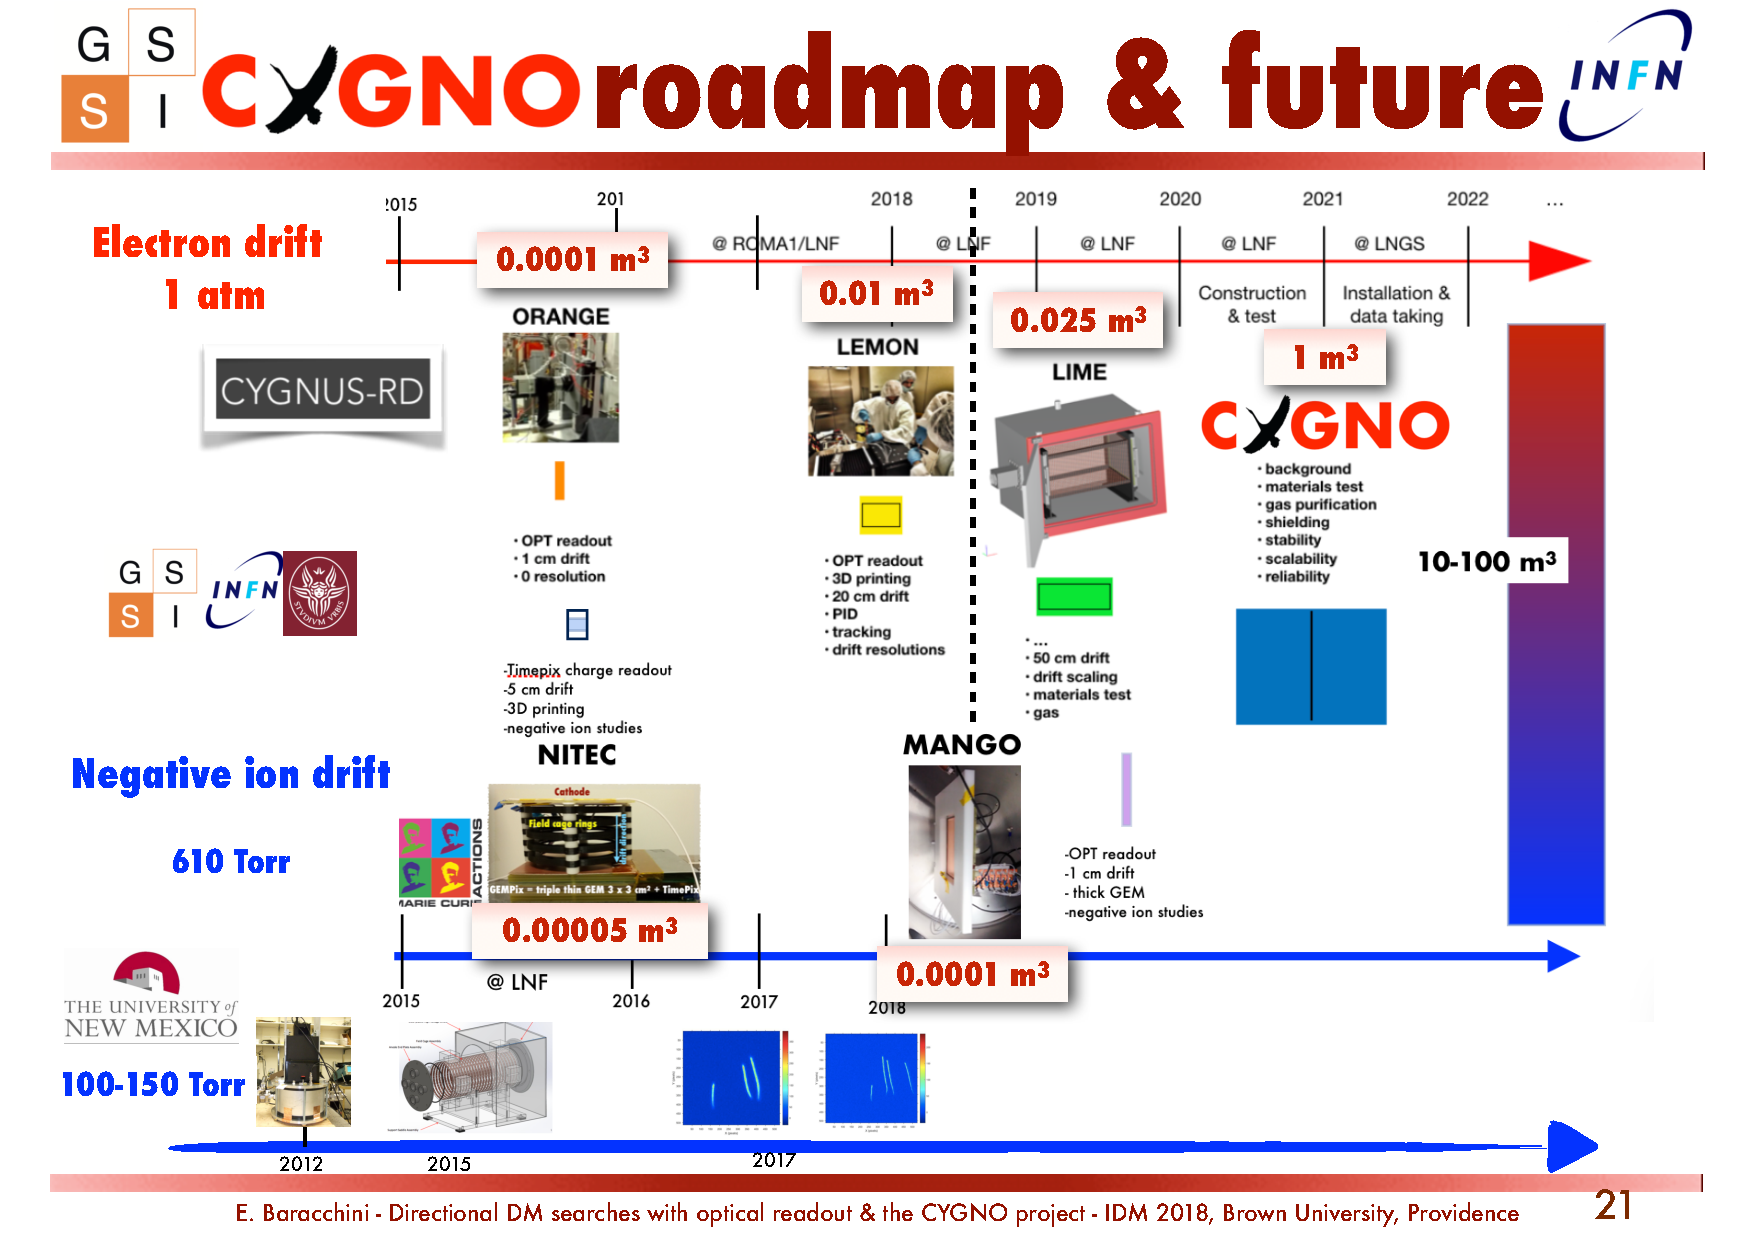
\includegraphics[width=0.89\linewidth]{cygno_IDM_2018_roadmapslide.pdf}
%    \caption{ROADMAP: da cambiare}
%      \label{fig:roadmap}
%\end{figure}

The roadmap details and synergies with other projects will be illustrated in the following. 

\subsection{CYGNO PHASE\_0: the LIME prototype}\label{sec:phase0}

The Long Imaging ModulE ({\it \lime}, in Fig.~\ref{fig:LIME_pic}) is equipped with triple 33 $\times$ 33 cm$^2$ thin GEMs (stretched on plexiglass frame to reduce radioactivity), amplifying a 50 cm drift length, for a total active volume of about 55~litres imaged by 4 small PMT and a single sCMOS. The new Hamamtsu ORCA-Fusion Camera was employed\footnote{https://www.hamamatsu.com/eu/en/product/type/C14440-20UP/index.html} with improved performance with respect to the Orca Flash (see Sec.\ref{sec:results}) in terms of reduced noise (0.7 versus 1.4 electrons), larger number of pixels (2304 $\times$ 2304 versus 2048 $\times$ 2048) and larger quantum efficiency (80$\%$ versus 70$\%$ at 600 nm). 
The choice of 4 PMT resides in the possibility of better reconstructing track position and inclination through center of gravity of the light signal from the 4 sides, strongly mitigating any possible pile up effect.

The gas volume is enclosed in a 10~mm thick plexiglass box, that provides gas tightness. The field cage is composed by copper rings, conveniently roundly shaped to avoid discharges, at a 1 cm pitch (see Sec.\ref{sec:phase1}).

In its underground installation LIME will be equipped with the same DAQ system and gas system envisaged to be employed for the realisation of PHASE\_1, currently under test.

\begin{figure}[!t]
\centering
 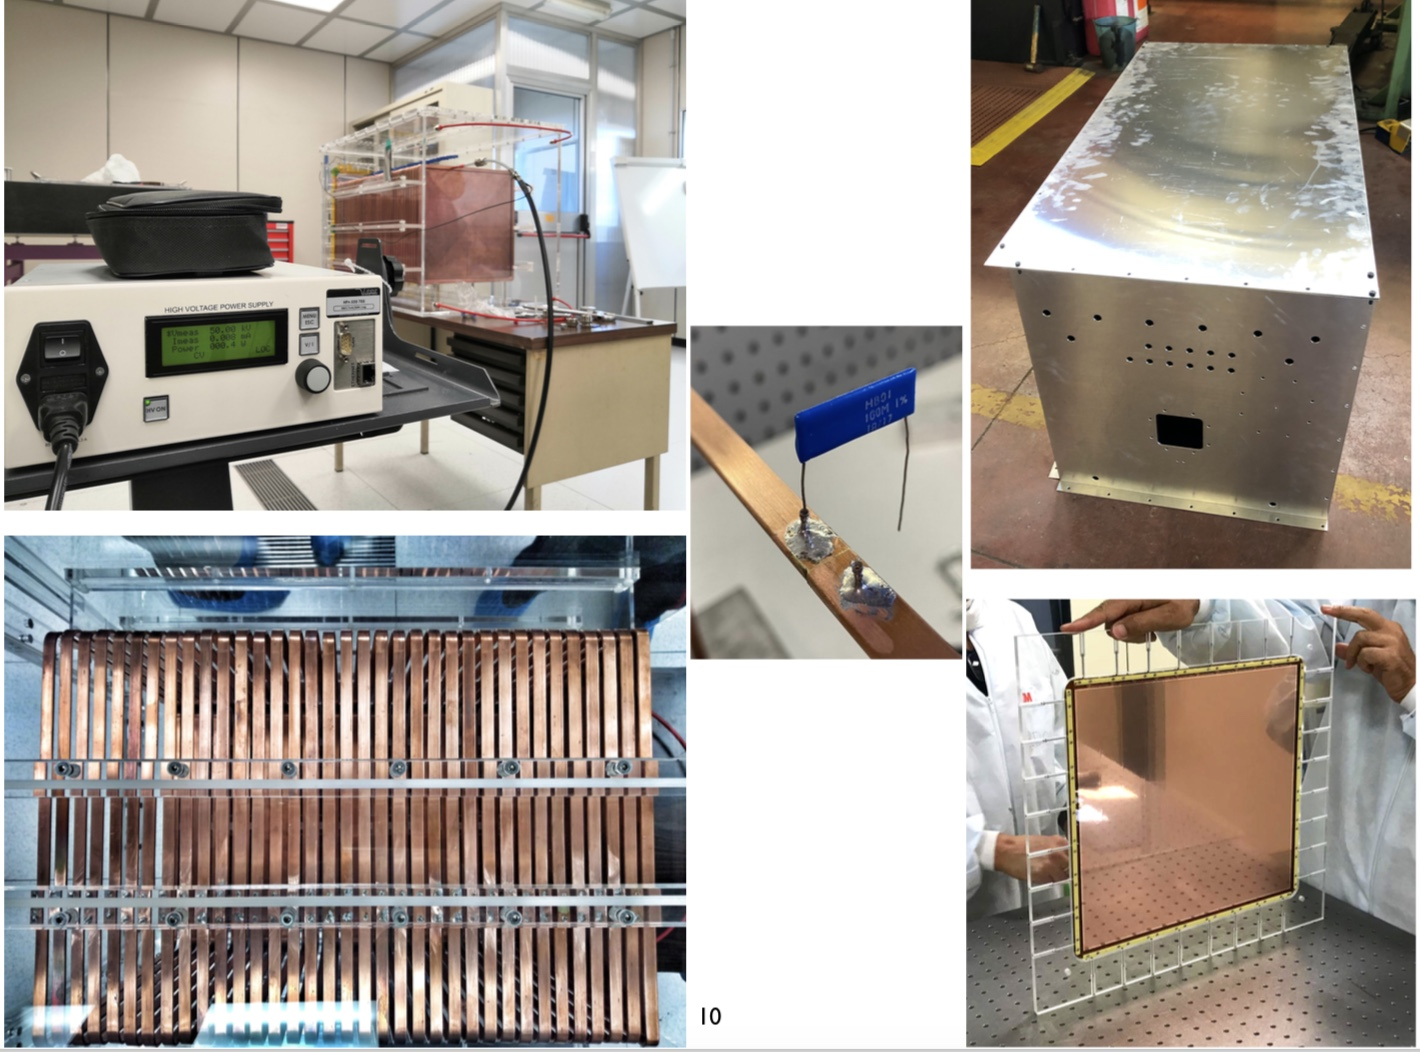
\includegraphics[width=0.6\textwidth]{LIME_pic.jpeg}
 \caption{Picture of the LIME detector assembly at Laboratori Nazionali di Frascati: top left with drift field and GEM operating at nominal voltages, bottom left detail of the field cage copper rings, center detail of the resistor soldered to the field cage ring, top right LIME inside the Faraday cage, bottom right detail of the triple GEM streatched with pullouts on a plexiglass frame.}
 \label{fig:LIME_pic}
 \end{figure}


A response of 1180 ph/eV (to be compared with 514 ph/eV obtained with \lemon, see Sec.\ref{sec:yield}) was measured effectively lowering our energy threshold of a factor 2. The energy resolution on the $^{55}$Fe peak is measured to be 14$\%$ across the whole 50 cm drift length, with full efficiency in the full 50~litres volume. LIME has been furthermore already operated for one entire month in He/CF$_4$ 60/40 at 1 atm, with its currents continuously monitored and logged, showing comparable stability to \lemon (see Sec.\ref{sec:stability}).

The PHASE$\_1$ demonstrator will be based on readout modules having the LIME dimensions and layout (see Sec.\ref{sec:phase1}). For this reason, its successful assembly and operation will be paramount to substantiate the efforts and confirm the scientific and technological choices towards the 1 m$^3$ detector. 

The installation at LNGS, completed with the PHASE\_1 auxiliary systems, will allow to test on realistic dimensions and operating conditions the construction and material options, and detector long term activity in the underground environment. 

In addition, two modes of operation  are foreseen at LNGS, each with its own specific scientific goal:

\begin{itemize}
    \item {\bf Environmental neutron flux measurement operation}. \lime~will be equipped with an electromagnetic background shielding of about 10 cm of Copper, to reduce external gamma backgrounds. The goal of this first stage is to demonstrate the capability to precisely track low energy nuclear recoils in an underground setup by measuring the environmental underground neutron flux with directionality. While already  fundamental for the successive PHASE$_1$ development, this measurement will provide a crucial input for any present and future rare events search experiment at LNGS.
    \item {\bf Internal electromagnetic background measurement operation}. An additional Water shielding of about 50~cm will be added to the Copper shielding, in order to avoid external neutrons interacting in the detector active volume. The combination of Water/Copper/Lead shielding must ensure a level of background contamination inside the detector smaller than the one expected from its internal components, that from current estimations are expected to be about 0.5 - 1 $\times$ 10$^5$ per year in [1,20] keV$_{ee}$ range (see Sec.\ref{sec:phase1}). With this configuration, it will be therefore possible to precisely assess the background assay to further minimise it through material and shielding choices for PHASE\_1. 
\end{itemize}

\begin{figure}[!t]
\centering
 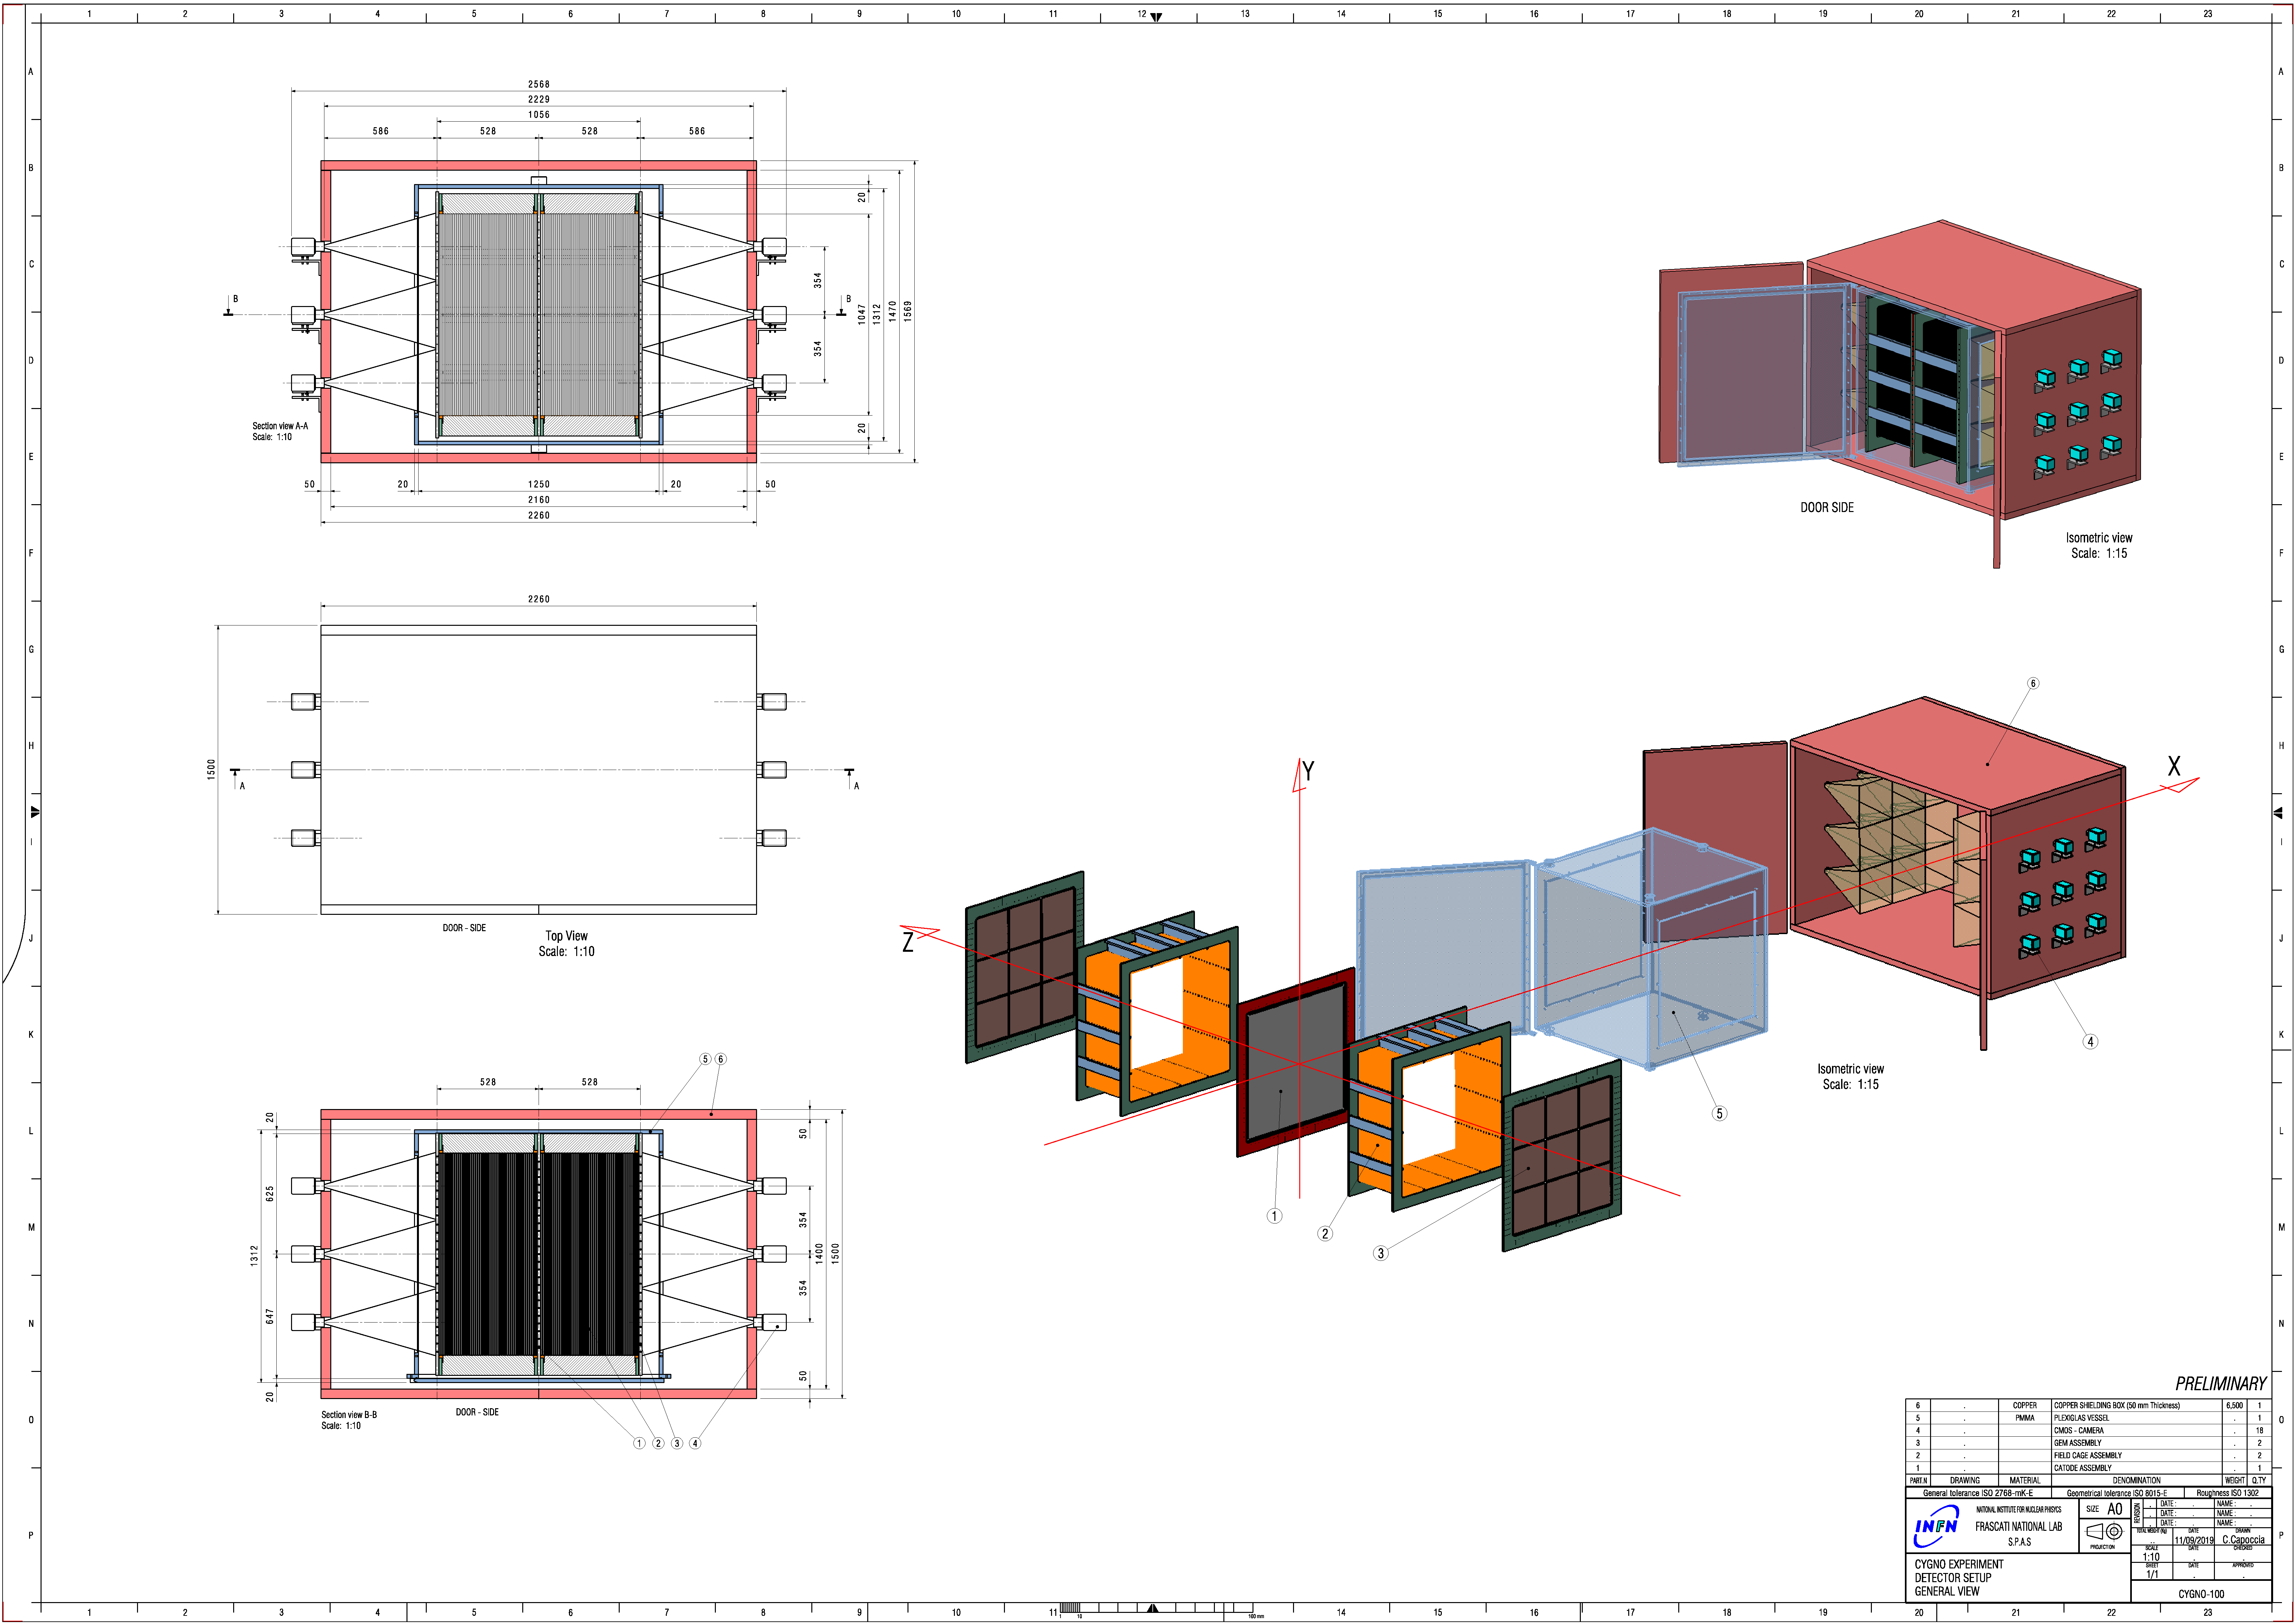
\includegraphics[width=0.7\textwidth]{CygnoDetector.pdf}
 \caption{CYGNO PHASE\_1 Sensitive Detector Layout}
 \label{fig:detector}
 \end{figure}
 
\subsection{CYGNO PHASE\_1: the O(1) m$^3$ demonstrator}\label{sec:phase1}
The PHASE\_1 detector will comprise of  O(1) m$^3$ active gas volume, with two back-to-back TPCs separated by a central aluminised mylar cathode following the DRIFT example \cite{Battat:2015rna}, able to minimise backgrounds induced from Radon Progeny recoils. 
%will be finalised once assigned the underground space at LNGS, whose final location is under discussion with the laboratory management. 
The exact PHASE\_1 detector sizes is still under discussion, anyway a 1 m$^3$ active volume will be discussed in this paper, schematically shown in Fig.~\ref{fig:detector},
with the consideration that the foreseen layout and auxiliary system can be directly and easily adapted to the definitive detector dimensions.

The active volume of the detector will be contained in a gas volume vessel (GVES), realized with PMMA to lower the material intrinsic radioactivity, gas contamination and ensure the electrical isolation from cathode and filed cage. 
The box will contain two field cages 500~mm long, separated by a central cathode. On the two endcaps, two arrays of triple GEM will be located, to amplify the signal generated in the gas. Each endcap will be readout by $N$ modules of $33 \times 33$ cm$^2$  area, each one equipped with a sCMOS and 4 PMT, identical to the LIME prototype of PHASE\_0, where $N$ depends on the final detector dimension. For a 1 m$^3$, 9 LIME-like modules are foreseen for each end cap, for a total of 18.

The GEMs will be assembled adapting the technique discussed in \cite{Colaleo:2015vsq}. The mechanical rigidity will be provided by the outer frame that will be anchored to the GVES. The outer frame will support the stretching screws pulling the GEMs to produce the necessary mechanical tension (0.1 N/m applied by mean of dynamo-metric screwdriver) to ensure flatness and homogeneous electric field between the foils \cite{Benussi:2015omy}. The assembled GEM stack will be inserted into the GVES through vertical slits, which will allow and easy substitution of a single GEM foil in case of damage.

%A finite-element simulation was developed to optimise the field cage design to maximise the uniformity of the drift field and to avoid discharges from sharp edges. Different shapes were considered for the electrodes (i.e. wires versus bars) and dimensions, as well as different configuration of dimension matching between the electrodes and anode and cathode (namely, rings perfectly matching GEM and cathode dimensions, or slightly larger, or slightly smaller). Wires perform clearly worse than bars, and a good compromise between the field uniformity and the maximum electric field between two subsequent electrodes (required to be below 20~kV/cm, a benchmark value for helium-based mixtures, to avoid avalanches and discharges) is found with a $6~\mathrm{mm} \times 2~\mathrm{mm}$ bar every $10$~mm. Moreover, simulations shows that deformations of the field at the cathode are minimized with electrodes slightly larger than the cathode (while no significative differences are observed at the GEM). 
%Wee are also considering the possibility of replacing the electrodes with a resistive foil (antistatic PVC, 0.2~mm-thick, $10 \times 10^{10}~\Omega/\msquare$ resistivity)
%$10 \times 10^{10}~\Omega/\msquare$ resistivity) that would give the best approximation of the ideal case of a surface with a continuous linear voltage drop~\cite{resistive_foil}.

The high voltage system has been conceived with the assumption of independent lines 
for each electrodes of the GEM foils, in order to ensure safe and reliable 
operation of the detectors. 
Since for a 1 m$^3$ $18 \times 3$ GEMs are foreseen, a total number of 108 independent high voltage channels has been considered for PHASE\_1. The baseline adopted solutions is based on boards equipped with 14 Floating Channels.

The DAQ system needs to be able to collect synchronized data from cameras and photodetectors and to handle the following specifications: 
\begin{itemize}
    \item camera exposure from 0.2 to 1 second (1 to 5~Hz frame rate);
    \item 10~MB of data per picture (5~MP, 16 bit per pixel); 
    \item 12-bit digitization of photodetector waveforms at $\sim 250$~MS/s in $\lesssim 1~\mu$s windows.
\end{itemize}
 Since sCMOS cameras data can not be used to develop a trigger, the only possible sources of signals to start data acquisition are from the photodetectors. The possibility of running either in trigger or trigger-less mode was also evaluated. 
 
% It was realised that in the first case almost all pictures would be collected, giving no real advantage with respect 
%to the trigger-less mode. The possibility of switching to the trigger mode will be considered only
%if it turns out to be advantageous, given the rates that will be observed in the experiment. According to the specifications above, a trigger-less DAQ system should be able to transfer up to 50 MB/s per camera, while the
%data load from the digitizers would be well below 1 MB/s per photodetector. If the cameras are readout by cutting-edge CameraLink PCI Express (PCIe) 3.1 frame grabbers, with a maximum throughput of 2.5~GB/s, a single 
%front end machine could in principle readout all 18 cameras foreseen for a 1~m$^3$ detector. Anyway, 

The acquisition will be distributed through a few 
machines to ensure stability of the system. To acquire fast photodetectors, digitization boards are considered. In this scenario, the bottle-neck for the acquisition would be the throughput to the disk, typically limited to O(200~MB/s),
and some pre-selection of the images by a farm of CPUs would be needed. 

%If the pre-selection algorithm requires 1 second to process an image, 10 CPUs are needed to handle the 10~Hz frame rate. The algorithm should reject $\sim 90\%$ of images if all CPUs have to write data on the same disk. This seems consistent with what expected from an underground, low activity environment such as LNGS, in particular with the external passive detector shielding.

\subsubsection{PHASE\_1 Shielding Scheme and Material Budget}\label{sec:back}

A \GEANT~based Montecarlo simulation reproducing a 1 m$^3$ detector as from the engineering design of Fig.~\ref{fig:detector} has been developed to study external and internal background and to optimise the choice of shielding and materials. 

The effect of the diffused external environmental $\gamma$ and neutron flux using as a reference the spectra measured at LNGS was studied. Different configurations of external passive shielding with layers of Copper, Lead and Water were studied with the goal of less than 10$^4$ gamma/year interacting in the target gas between 1 keV and 20 keV. The choice of this benchmark is backed up by indication from measurements\cite{Riffard:2016mgw,Phan:2015pda} and simulation within the CYGNUS collaboration\cite{Vahsen:2020pzb} that a TPC with 3D readout can reach a 10$^5$ gamma/year rejection factor at O(keV). 

While the use of Pb can significantly reduce the overall setup dimensions, the simulation showed that this configuration would require archaeological Lead in order not to induce additional background from the shielding, therefore largely raising the cost of this layer. A cost-benefit optimisation of the shielding layer materials and thicknesses was hence developed, identifying 2 m of Water + 5 cm of Copper as the optimal configuration. This shielding provides an attenuation of about 10$^{-7}$ for external gammas and 5 $\times$ 10$^{-5}$ for external neutrons, reducing the number of expected electron recoils in the active volume below 10$^3$ cpy (with O(1) cpy nuclear recoils) in the range 1-20 keV. 

\begin{table}[t]
    \centering
    %\scalebox{0.9}{
    \resizebox{\columnwidth}{!}{
   % \begin{tabular}{c|c|c|c|c|c|c|c|c}
    \begin{tabular}{c|c|c|c|c|c|c}
    Component & $^{238}$U ($^{234m}$Pa)  & $^{238}$U ($^{226}$Ra) & $^{235}$U  & $^{232}$Th ($^{228}$Ra) & $^{232}$Th ($^{228}$Th) &  $^{40}$K  \\ % & $^{137}$Cs [Bq/kg] & $^{60}$Co  [Bq/kg]   \\
\hline
\hline
Camera body [Bq/pc] & 7 & 1.8 & 0.4 & 2.1 & 2.1 & 1.9 \\ % & 0.04& 0.005 \\
Camera lens [Bq/pc] & 0.9 & 0.41 & 0.031 & 0.08 & 0.08 & 11 \\ % & 0.046 & 2.44\\
GEM foil [Bq/$m^2$] & < 0.104 & 0.004 & < 0.002 & < 0.004 & < 0.002 & < 0.045 \\ % & 0.008 & 0.007 \\
Acrylic [Bq/kg] &  &  0.003 &  & 0.005 & 0.004 & 0.035 \\ % & & \\
 \hline
 \hline
    \end{tabular}
    }
    \caption{Measured activity of the internal detector components expected to produce the largest backgrounds in the active volume. The isotopes in parentheses indicate the activity from that particular part of the decay chain. Upper limits are given at 90\% confidence level.}
    \label{tab:camera_radio}
\end{table}

 

For the evaluation of the internal backgrounds generated by detector materials, the natural gamma radioactivity of the components expected to give the largest contributions was experimentally measured with high purity Germanium detectors thanks to the support of LNGS Special Techniques Service and are reported in Table \ref{tab:camera_radio}. 

Regarding the GEMs, the major source of background is found to come from the frames rather than the foils themselves. For this reason, in the LIME prototype of PHASE\_0 the triple $33 \times 33$ cm$^2$ GEMs were mounted and stretched on low radioactivity acrylic frames, with same technique foreseen to be applied to the PHASE\_1 detector. 

For what concerns the sCMOS optical system, a large $^{40}$K contamination was observed in the objective glass. Suprasil was selected as an alternative material for the fabrication of the lens, for an expected $\sim$ 10$^4$ reduction of the contribution from this item. An overall activity of less than 50 mBq/kg was found in recent measurements performed on a sample at LNGS, confirming the very good properties of this material.

sCMOS cameras have never been employed yet in DM searches, and therefore their intrinsic radioactivity has never been studied or optimised in this context. For this reason, an extensive program working in close contact with sCMOS camera producer companies and with LNGS Services to assess this aspect within our experimental approach has started. Gamma spectroscopy of several sCMOS cameras as a whole was performed, including models from companies different from Hamamatsu, and verified that all displays similar activities in the O(10) Bq/piece. The measured activities of the Hamamatsu Orca Fusion are shown in Table \ref{tab:camera_radio}. A camera was disassembled it in 20 different pieces, which are currently under measurement in order to pin point the components introducing the larger radioactivity contamination and possibly substitute them with cleaner options. Given the very large sCMOS activity, in the PHASE-1 design they are foreseen to be shielded by the 5 cm Copper layer on all sides, except for the one facing the GEM.

Starting from these considerations, a background evaluation for a 1 m$^3$ PHASE\_1 detector was developed, that includes the external gamma and neutron flux contribution with the Copper + Water shielding discussed above, and the radioactivity contribution of the main internal components. For this last,  the values measured at LNGS for GEMs, camera objective, camera body and acrylic for the gas vessel, and data from literature for the Cu of the cathode and the field cage rings [CIT]  were employed. This study showed that O(10$^3$) nuclear recoils and O($10^6$) electron recoils per year are expected in the sensitive volume, with energy in the 0-20~keV range. It must be noted that all the nuclear recoils are produced by the GEMs and are absorbed in the gas within 5 cm from them. As it is described in Sect.~\ref{sec:track}, by exploiting the effect of diffusion in gas, the track absolute distance from the GEM can be evaluated with a resolution better than 20\%. Therefore, this NR background is expected to be reduced to zero with a suitable selection on the drift distance, without a significant reduction of the detector fiducial volume. The largest amount of electron recoils is produced by the sCMOS cameras, if the camera objective can me made of a clean material, and at a second order by the GEMs.

This study represents the current evaluation of the expected backgrounds for a 1 m$^3$ detector, which can be further minimised by the material screening and the study of the sCMOS intrinsic radioactivity ongoing, and do not therefore need to be considered the ultimate achievable performances.




%Natural radioactivity in the experimental hall can produce events that will represent a background to the searches of CYGNO.
%Main and most dangerous background contributions are represented by electrically neutral particles that can enter interact directly in the gas producing nuclear recoils or electron recoils very similar to signals due to rare events (such as neutrino or WIMP interactions).
%In order to reduce it, the demonstrator will be provided of external shields. A detailed simulation of the effect of the neutron and photon fluxes present in the experimental hall, based on the most recent measurements \cite{bib:lngs_neutron, bib:lngs_gammas}, was carried on in \GEANTfour~\cite{bib:geant}.

%Different shielding solution were tested in order to find the one able to significantly reduce the number of events due to external radioactivity while requiring reasonable material budget and costs.

%Table \ref{tab:shield} summarises the main results:
%\begin{itemize}
~%    \item copper was chosen to effectively screen from external gammas. It was preferred to the less expensive and more dense lead because of its high radio-purity level commercially availability;
%    \item distilled water represents a very good solution to moderate neutrons and make them being efficiently captured in copper.
%\end{itemize}

%\begin{table}[h!]
%\centering
%\caption{Background rates. Copper costs assuming~(10~\EUR{}/kg) \\ 
%for CYGNO-1.0: $110\times110\times220$~cm$^3$ internal shielding size; 0.58~m$^3$ for 5~cm;}
%\\
%https://docs.google.com/spreadsheets/d/1bgR1mm6i2Z_AnlDX0mlHRTFYeDGw-dXvEvLyFloiAyc/edit#gid=0
%\begin{tabular}{|c|c|c|c|c|c|} 
% \hline
%Detector        & Water/Copper   & Water         &  Copper & [1-20]~keV & Label\\
%Volume (m$^3$)  & Thickness (cm) & Cost (k\EUR{})&  Cost (k\EUR{}) & cpy &    \\
%\hline
%\hline
%1 & - & - & 1  & & & 1 $\times 10^{10}$ \\
%\hline
%1 & 250/5 & & 150 & 1 $\times 10^{2}$ \\
%\hline
%1 & 200/5 & 160 & 160 & 5 $\times 10^{2}$ & A \\
%\hline
%1 & 100/5 & 60 & 160 & 2 $\times 10^{5}$ & B \\
%\hline
%1 & 85/5 & & 150 & 1 $\times 10^{6}$ \\
%\hline
%1 & 50/5 & & 150 & 8 $\times 10^{6}$ \\
%\hline
%\hline
%\end{tabular}
%\label{tab:shield}
%\end{table}

%In the case B, the rejection capability provided by the experimental approach will allow to reduce the number of unavoidable background events due to external radioactivity to few thousands per year.
%Therefore, the solution A would be preferable in case of enough available room even if total cost of shielding would be around 350 k\EUR{}.

%\subsection{Internal Background Simulation}

%To quantify their effect, the radioactivity of all detector components and material was measured and included in the \GEANTfour simulation. 
%Largest contributions to detector background were found from:

%\begin{itemize}
%    \item Camera: with an activity of about 3 Bq/kg due to $^{238}$U;
%    \item Lens:  with an activity of about 4 Bq/kg due to $^{238}$U and 50 Bq/kg due to $^{40}$K;
%    \item GEM:   with an activity of about 0.16 Bq/kg due to $^{238}$U and 0.36 Bq/kg due to $^{40}$K;
%\end{itemize}

%Main consequence of those activities are 10$^3$ nuclear recoils and $2\times 10^3$ electron recoils per year in the sensitive volume, with energy in the 0-20~keV range.

%Nuclear ones are all due to GEMs and are absorbed in the first 5 cm. As it is described in Sect.~\ref{sect:track}, by exploiting the effect of diffusion in gas, the distance of the events from the GEM can be evaluated with a resolution better than 20\%. Therefore, NR can be easily rejected with a suitable selection on the detector fiducial volume.

%A rejection factor of 10$^2$ is already achieved in CYGNO prototypes for electron recoils with about 6~keV energy (see Sect.~\ref{sect:rej}) and there is room for improvements (see for example \cite{bib:recoil}). Assuming an exponential increase of the RF with electron energy, an average value of 10$^4$ can be obtained in the 0-20 keV energy range.

%Given the expected rates, a number of $10^2-10^3$ ER events are expected to pass the selection per year.

%\subsection{CYGNO PHASE 2: the O(100) kg Exposure  Experiment}
\subsection{CYGNO PHASE\_2}

%A 50 kg scale CYGNO detector would be able to give a significant contribution to direct DM searches in the low 1-10 GeV WIMP mass region for both SI and SD coupling while paving the way for a directional DM experiment at the ton-scale, distributed over several underground laboratories (see Sec.\ref{sec:cygnus}). It could furthermore provide the first directional measurement of Solar neutrinos from the pp chain, possibly extending to lower energy the Borexino measurement, as will be illustrated in Sec.\ref{sec:neutrino}. 

The experimental results and sensitivities measured on the 1 m$^3$ demonstrator, will provide crucial information about the possibility of proposing a larger experiment.

A  development of such a detector in terms of intrinsic background minimisation and tracking performance, would of course require an improved scalable design in terms of active volume versus readout area and costs. The possible improvements include, but are not limited to, the following:


\begin{itemize}
\item development of custom sCMOS sensors, with faster frame rate, lower noise, improved granularity, improved QE over a wider wavelength spectrum and reduced intrinsic radioactivity. 
\item enhancement of the light yield through optimised amplification stage with reduced intrinsic radioactivity, possibly including the exploitation of the electroluminescence recently demonstrated by the CYGNO collaboration in He/CF$_4$ \cite{Baracchini:2020dib}; 
\item optimisation of the optical configuration, to possibly strongly reduce the costs. Due to the very low rate the probability to have multiple events in different area of the detector is very low. This implies that many areas of the GEMs active surface can be observed simultaneously by the same sensor by multiplexing the image with  mirrors or collecting different area in on the same focus point with collimators. Studies of this concept are ongoing;
\item reduction the intrinsic detector material radioactivity, with the lesson learned after the results obtained with PHASE-1.
\item boost of tracking performances through the development of innovative gas mixtures for optical readouts that will be illustrated in the following sub-section.
\end{itemize}



\subsection{INITIUM: an Innovative Negative Ion Time projection chamber for Underground dark Matter searches}

The challenging goal of INITIUM is to develop Negative Ion Drift (NID) operation within the CYGNO optical approach. 

Negative Ion Drift is a peculiar modification of conventional TPCs (NITPC) that involves the addition to the gas of a highly electronegative dopant \cite{Martoff:2000wi, Ohnuki:2000ex}. In this configuration, primary electrons liberated by the track while ionising the gas are captured at very short distances <10-100 $\mu$m by the electronegative molecules, creating negative ions. These anions drift to the anode, where their additional electron is stripped and gives rise to a standard electron avalanche. 
%Thanks to the anions mass being much larger than electrons, their diffusion is reduced to the thermal limit without the need of magnetic fields, achieving a dispersion of $\sim$ 1 mm/m \cite{Martoff:2000wi, Ohnuki:2000ex} (to be compared to $\sim$ 20 mm/m expected for conventional electron drift). This characteristic allows for the use of longer drift distances, combined with improved tracking performances. Recently, a new remarkable feature has been observed in negative ion gas mixtures: the presence of multiple charge carriers in the time signal, with different masses \cite{Snowden-Ifft:2014taa}. 
Since anions mobility depends on the mass, the difference in time of arrival of different anions effectively provides a measurement of the position of the event along the drift direction. Full 3D detector fiducialization can be obtained exploiting this information (i.e. DRIFT), and background-free operation over 1 m$^3$ \cite{Battat:2016xxe}. Thanks to these two features, NITPC readout planes can image a larger volume than conventional TPC approaches, resulting in lower backgrounds and costs for unit mass.

SF$_6$ has been recently demonstrated to work very well as negative ion gas between 20 and 100 Torr, including the possibility of high gains and fiducialization via minority charge carriers \cite{Phan:2016veo, Ikeda:2020pex, Lightfoot:2007zz}. Compared to the high vapour pressure, low flash point and low explosive mixture in air of the CS$_2$ employed by DRIFT, SF$_6$ has the substantial advantages of much more safer handling, combined with easier Radon purification and re-circulation, while at the same time increasing the target Fluorine mass. The studies proved for the first time the feasibility of NID at nearly atmospheric pressure (0.8 atm) with He/CF$_4$/SF$_6$ at 360/240/10 Torr with triple thin GEMs and charge pixel readout (Timepix) \cite{Baracchini:2017ysg}.

INITIUM goal is to develop a scintillating He/CF$_4$/SF$_6$ based gas mixture at atmospheric pressure with low content of SF$_6$ for NID within optical readout. If NID can be achieved within the optical approach, tracking could be improved by the possibility of reconstructing the track shape along the drift direction by sampling the recorded light at a kHz frame rate. At the moment such high rate can be met only by cameras with low resolution and high noise, not yet suited for low energy rare events searches. Nonetheless, given the fast development of the CMOS technology, advancements in short time are possible which could open the door to this possibility.

%It appears therefore evident how the CYGNO and INITIUM efforts share significant synergies along many aspects of their development, reflected also by the research teams involved in the projects.


\section{CYGNO Scientific Goals and Expected Physics Performances}\label{sec:physics}

%CYGNO's goal is to develop a TPC with  high precision 3D tracking capabilities, sensitive to the direction and the ionisation profile (i.e. dE/dx) of low energy recoiling nuclei \underline{and} electrons. This feature not only offers strategic means for particle discrimination and a positive identification of a DM signal, but opens also the possibility to investigate other physics cases involving either NR \cite{Vahsen:2020pzb, Baracchini:2020owr} or ER \cite{Seguinot:1992zu, Arpesella:1996uc} directional signatures. 

%In this section, wee will discuss in details the expected sensitivity of CYGNO PHASE 1 to WIMP searches and the tools wee developed to evaluate it (Sec.\ref{sec:wimp}) and wee will give an overview of the experiment potentialities towards additional directional searches.

%Here wee will briefly illustrate the potentialities for directional solar neutrino measurement (feasibility study under development) 

\subsection{WIMP-like DM searches at low masses through nuclear recoil signature} \label{sec:wimp}

A statistical analysis based on the Bayesian approach to evaluate CYGNO PHASE\_1 sensitivity to WIMP searches in presence of background was performed. As input our current expectation of the detector performances, extrapolated from the experimental results obtained with prototypes discussed in Sec. \ref{sec:results} was employed together with the background simulations illustrated in Sec.\ref{sec:back}.  

In order to establish the Credible Interval (CI) of the sensitivity limits,  fake experiments were simulated by extracting events according to the expected measured quantities, including detector effects. From these, the number of DM signal event posterior probability is evaluated and translated into a limit in the cross section versus mass parameters space.

CYGNO will measure both event energy and track directions simultaneously, and the two pieces of information will be combined into a combined fit for the final analysis. Nonetheless, since the angular distribution discriminating power is significantly stronger than the energy spectrum shape, in this sensitivity study only the first one is considered for the sake of simplicity. 

It is important to notice how the angular distributions strongly depend on the energy threshold and the target nuclei. In this work an energy threshold of 1 keV$_{ee}$ is assumed, backed up by the published results \cite{bib:fe55} and the improved results obtained with PHASE\_0 LIME prototype (see Sec.\ref{sec:phase0}). In order to translate this into nuclear recoils energy, a SRIM simulation was developed to evaluate the quenching factor (QF) for the elements in our gas mixture. The QFs for H, He, C and F in He/CF$_4$ 60/40 at 1 atm as a function of the nuclear recoil energy E[keV$_{nr}$] is shown on the left of Fig.~\ref{fig:QF_Probele}. This results in a energy thresholds of 2.14 keV$_{nr}$ for He, 3.12 keV$_{nr}$ for C and 3.74 keV$_{nr}$ for F.

\begin{figure}[!t]
\centering
 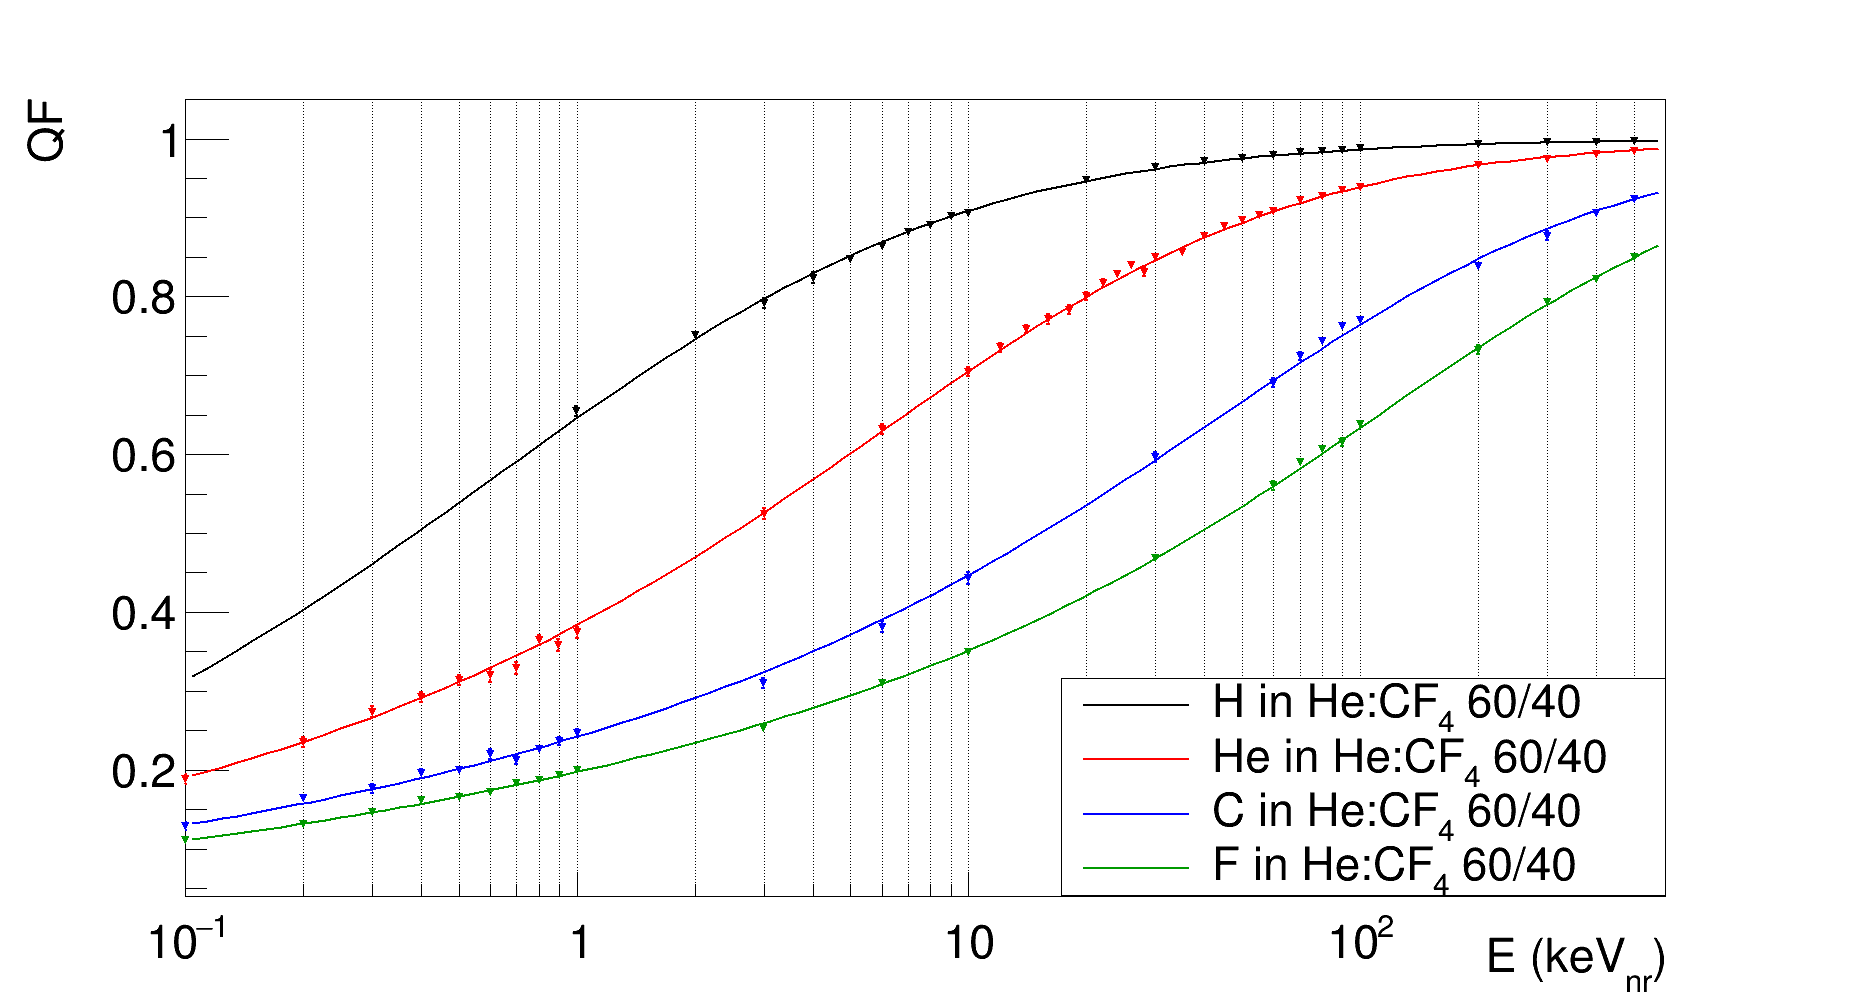
\includegraphics[width=0.35\textwidth]{QF.png}
 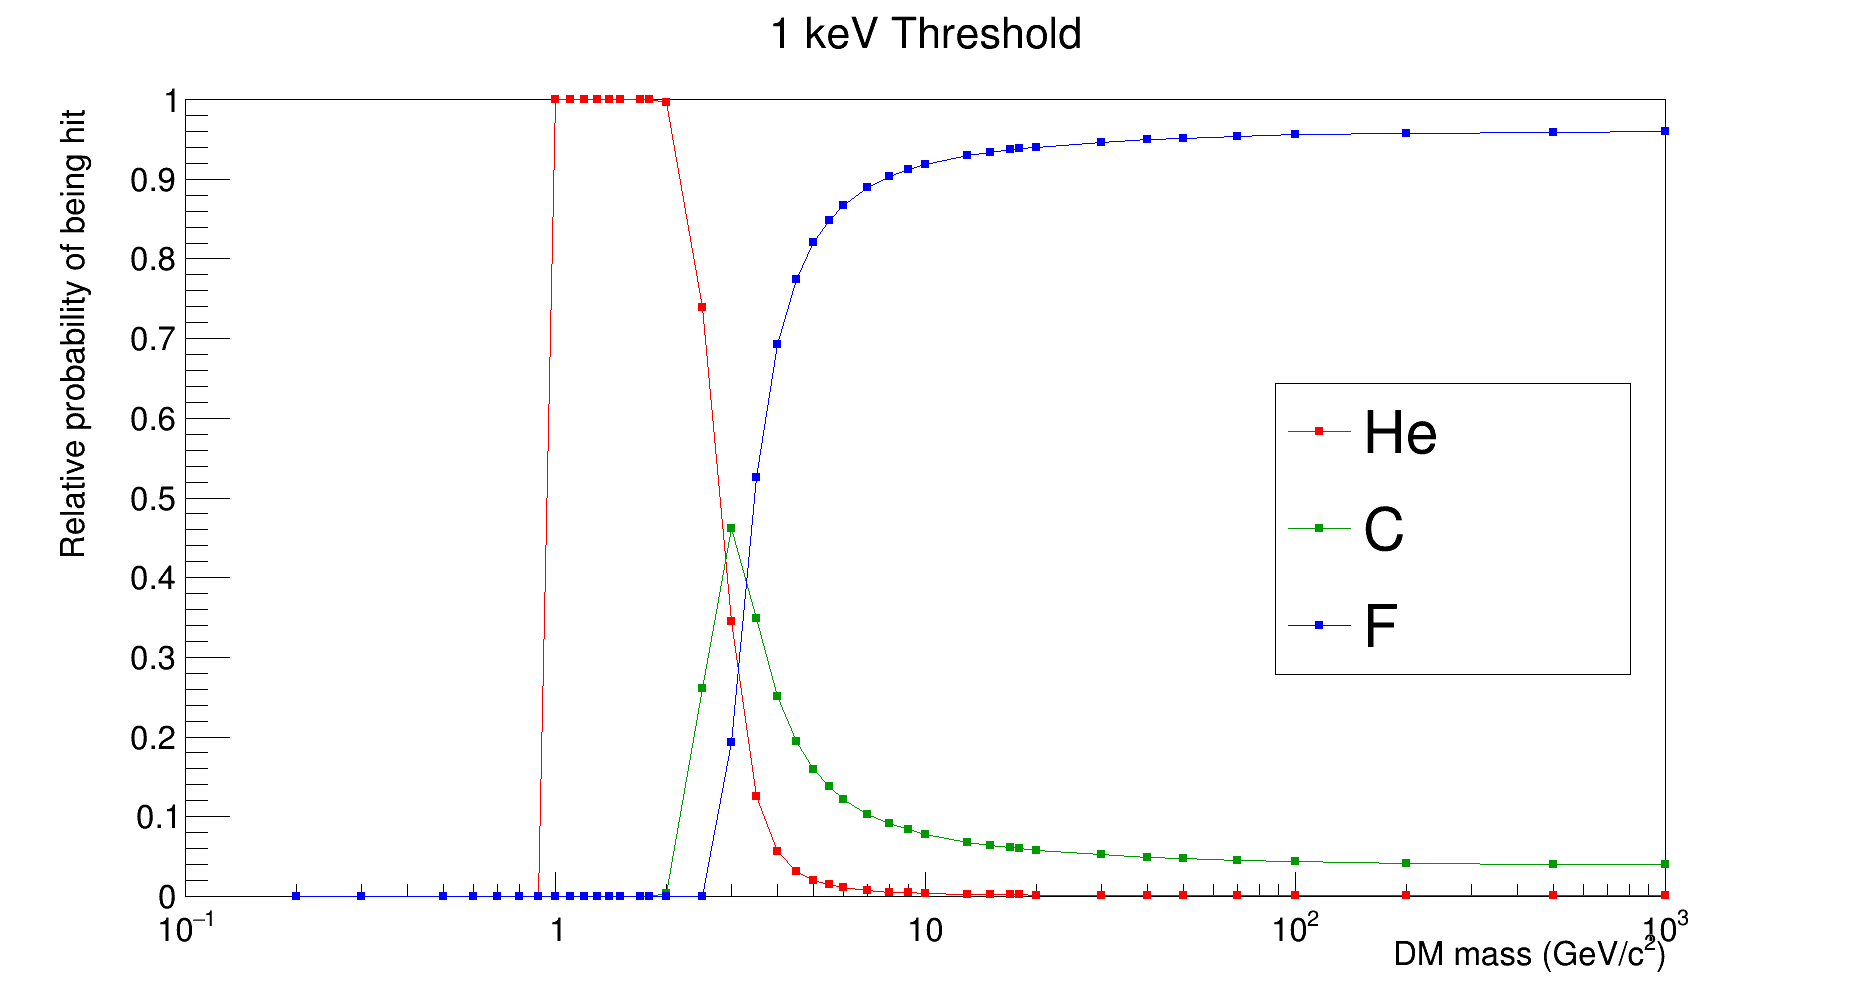
\includegraphics[width=0.35\textwidth]{Prob_hitting.png}
 \caption{Left: quenching factor values for different elements in a 60/40 He/CF$_4$ as a function of the nuclear recoil energy E[keV$_{nr}$]. Right: relative probability of nuclear recoils being detected as a function of the DM mass. The energy threshold is 1 keV$_{ee}$ and the quenching factor corrections are included.}
 \label{fig:QF_Probele}
 \end{figure}


It is interesting to notice that, due to the detector target being a mixture of different elements and to the kinematic of the expected DM-nucleus interactions, each element has a different probability of being detected depending on the DM mass. 
This is shown on the right of Fig.~\ref{fig:QF_Probele} and is properly taken into account in the estimation of the experiment sensitivity. The region of the DM velocity distribution accessible to detection is limited at lower values by the energy threshold and at higher by the local escape velocity. Thus, at lower DM masses, being the window of DM velocity distribution accessible very small, the detection of an element is strongly susceptible to its energy threshold. Therefore, helium detection dominates the early part of the figure and the rising probabilities of carbon and fluorine reflect their different thresholds. At higher DM masses, when  the window is quite large, the A$^2$ term in the rate calculation prevails, rendering fluorine the most detectable element. Figure~\ref{fig:QF_Probele} displays also the minimum DM mass detectable by each element, that is 0.97 GeV/c$^2$ for He, 1.89 GeV/c$^2$ for C and 2.55 GeV/c$^2$ for F recoils.
%This is a consequence of the fact that the region of the DM velocity distribution accessible to detection is limited at lower values by the energy threshold and at higher by the local escape velocity. This feature is shown in Figure \ref{fig:Probele} and is properly taken into account in the estimation of the experiment sensitivity. Figure \ref{fig:Probele} displays also the minimum DM mass detectable by each element, that is 0.97 GeV/c$^2$ for He, 1.89 GeV/c$^2$ for C and 2.55 GeV/c$^2$ for F recoils.


 
 While the evaluation of our approach about the directional performances on low energy nuclear recoils is still under study, from literature \cite{Nakamura:2012zza} and from the simulation within the CYGNUS effort \cite{Vahsen:2020pzb} an angular 
resolution of 30 deg in the whole 
detectable range can be assumed.
We furthermore recognise the capital importance of track sense recognition, as discussed, among the many, in \cite{Mayet:2016zxu, Vahsen:2020pzb}, but for the sake of simplicity full head-tail recognition is assumed down to the 1 keV$_{ee}$ energy threshold.
 
 
 The background angular distribution will be known very well only once it is measured during data taking. It is foreseen to be partially isotropic, coming from the outside the shielding assembly, and partially structured due to presence of internal radioactive material. However, once transformed into Galactic coordinates (taking into account the rotation of the Earth and the motion of the Sun) even these structured components should dilute and the overall distribution will be isotropic at first order.\\
The signal distributions were calculated in Galactic coordinates, starting from \cite{bib:LEWIN199687,bib:Gondolo_2002,bib:baxter2021recommended}, neglecting the motion of the Earth as it was shown to have secondary relevance on the angular distribution. Possible shapes of the recoil distribution are shown in 2D Galactic Coordinates in Fig.~\ref{fig:spectra2D}, where it is clearly visible its an-isotropic nature. The final shape of the distribution strongly depends on three elements: the DM mass, the element hit and the energy threshold. With the chosen settings for the analysis, the angular distributions tend to be strongly peaked at low masses and more spread at heavier masses, where there is no angular region forbidden by kinematics.
\begin{figure}[!th]
  \centering
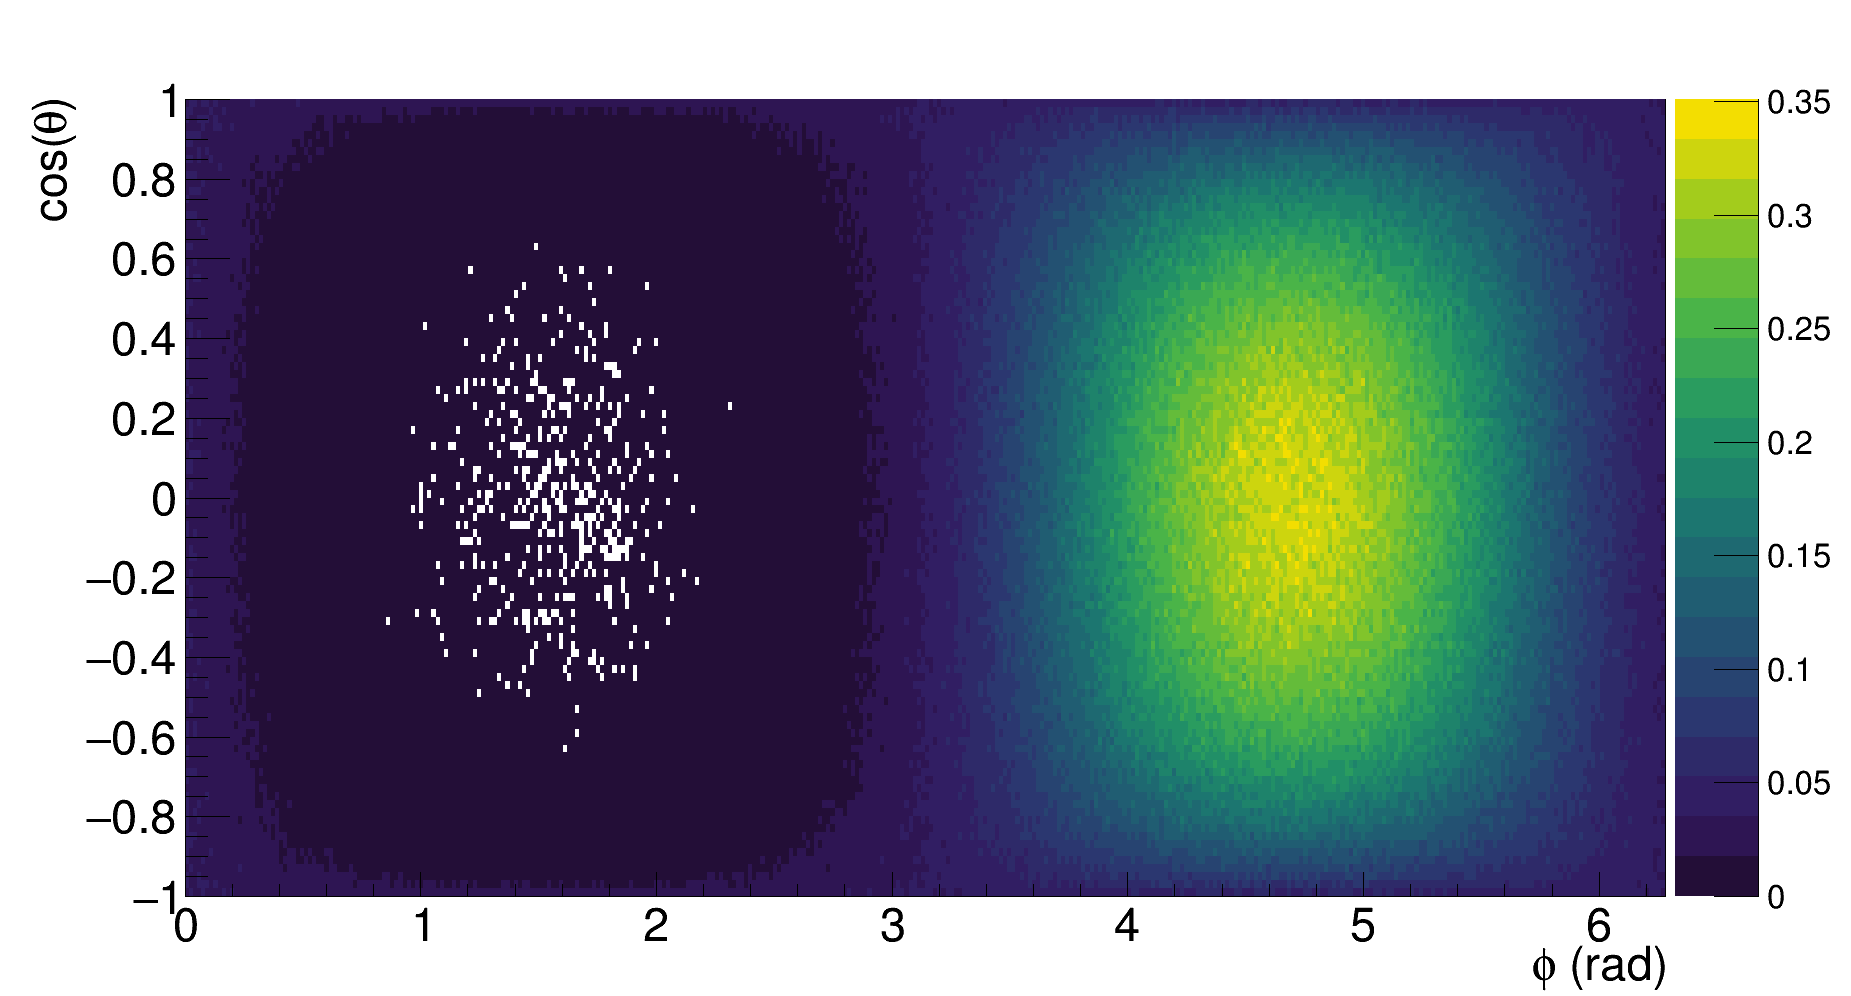
\includegraphics[width=0.36\textwidth]{Heliumrecoil_10GeV.png}
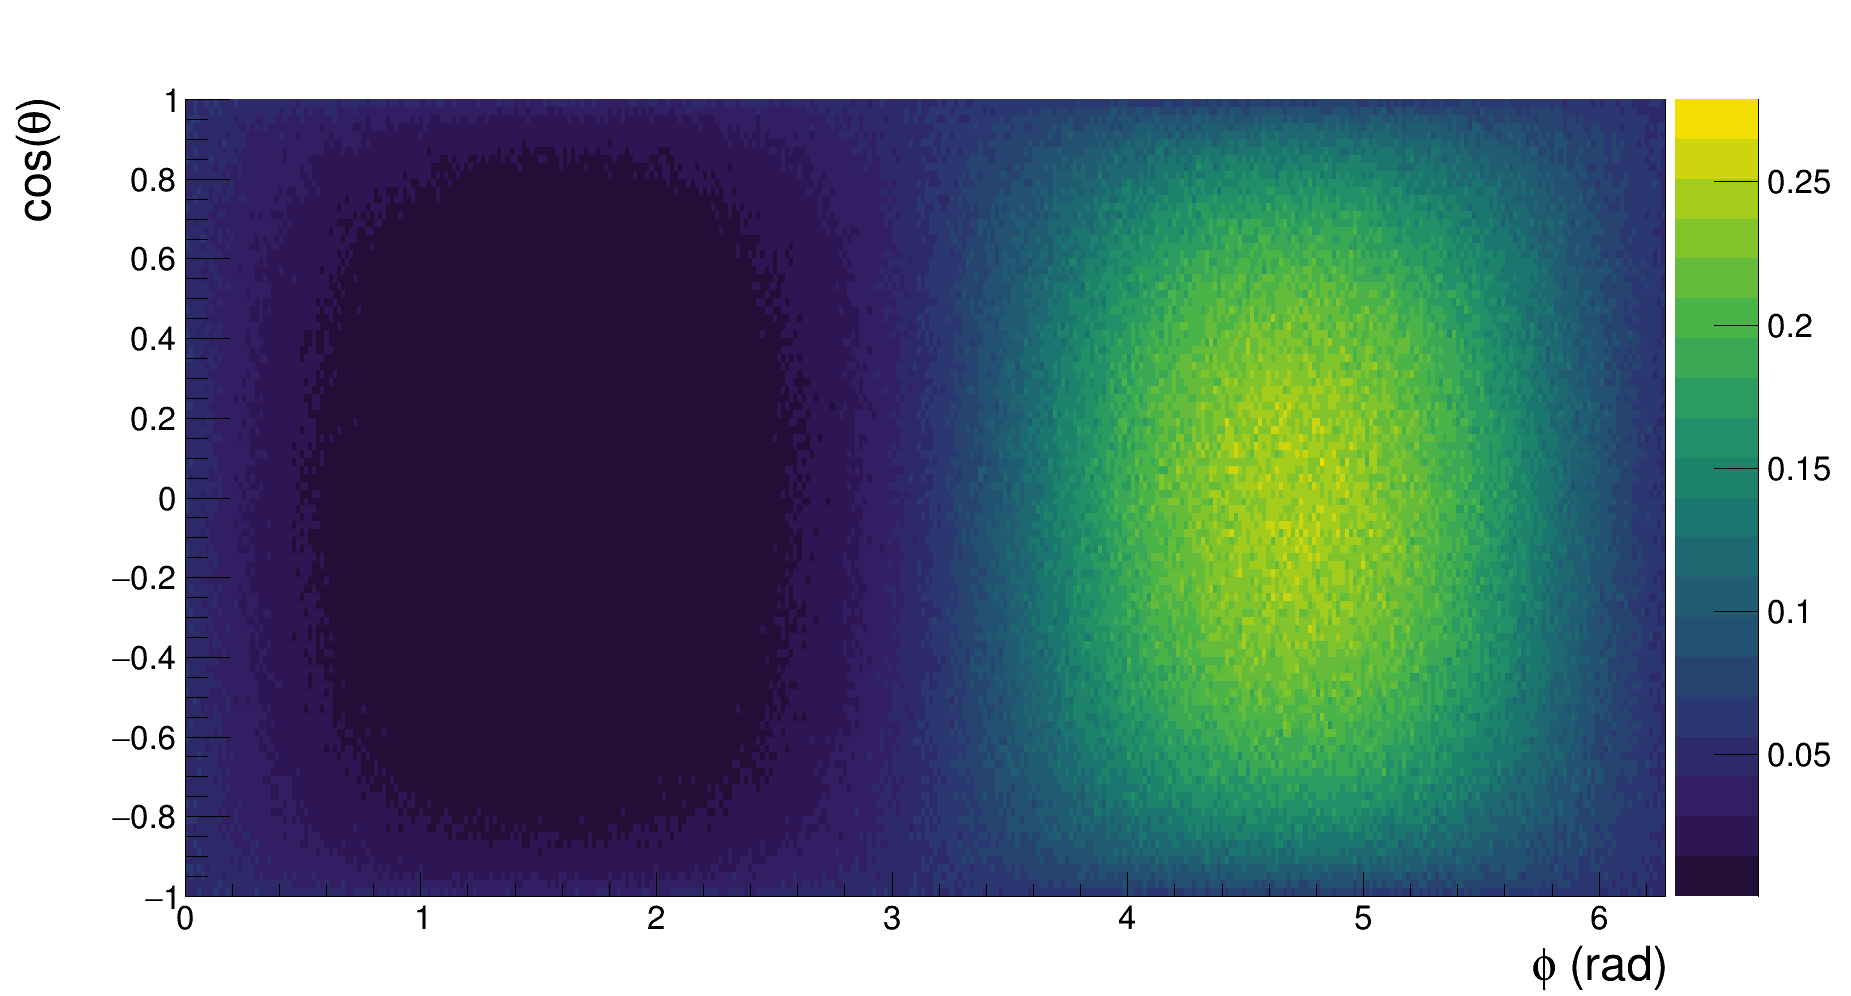
\includegraphics[width=0.36\textwidth]{WIMP_F_100GeV.png}
\caption{Two examples of the angular distribution of recoils due to DM in Galactic coordinates. On the left Helium recoils induced by 10 GeV/c$^2$ DM. On the right Fluorine recoils induced by 100 GeV/c$^2$ DM.}
 \label{fig:spectra2D}
\end{figure}


As it is shown in Sec.\ref{sec:back} the foreseen PHASE\_1 detector layout and shielding will result in about 10$^3$ NR and 5 $\times$ 10$^5$ ER background events due to material radioactivity in the [0,20] keV range per year. All the NR are expected to be rejected through fiducialisation along the drift direction.  A ER rejection factor (RF) of 10$^2$ has been achieved in CYGNO prototypes for electron recoils with about 6~keV energy (see Sect.~\ref{sect:rej}) and there is room for improvements (see for example \cite{bib:recoil}). Assuming an exponential increase of the rejection factor with electron energy, an average value of O(100) background events per year can be expected in the 1-20 keV energy range, in line with what discussed above \cite{Riffard:2016mgw,Phan:2015pda}. 

Given the uncertainties in these estimations and the large possibility of improvements in terms of tracking with more sophisticated approaches, the CYGNO PHASE\_1 sensitivity with a background rate ranging from 10 to 10000 events per year was evaluated. 



\subsubsection{WIMP search Limits Evaluation and Results} \label{sec:bayes}
%In this section, wee discuss how to estimate CYGNO PHASE 1 90\% Credible Interval in the cross-section-DM mass parameters space from the simulated fake experiments and the sensitivity limits obtained in the hypothesis that only backgrounds event are detected.

For the signal prior probability, since the actual value of the cross-section of DM with protons is not known, it is difficult to produce articulated priors without risking biases. For this reason, a simple flat distribution between 0 and 1000 was used to extract the expected number of signal events. Indeed, events per year is a non negative defined variable and due to current limits in the DM community, it is hardly believable that more than 1000 events per year would be produced in the CYGNO detector.\\
Since the number of events surviving the signal selection is expected to be predictable with a relative good confidence (especially after the measurements foreseen in PHASE\_0), for the  background events  a Poissonian prior centered at 10, 100, 1000 and 10000 was assumed to reflect possible different background scenarios.

For each scenario, the actual number of events is randomly extracted from this Poissonian distribution and a direction is assigned to each, randomly sampling the background angular distribution. After applying a Gaussian smearing to account for the resolution, an histogram representing the measured event direction in Galactic coordinates is filled, with its binning reflecting the angular resolution. In the hypothesis of only background, no events for the WIMP-induced signal recoils are added.\\

Once the data sample is prepared, the profile likelihood function is evaluated starting from the following formula:
\begin{equation}
\label{eq:likelihood}
 p(\boldsymbol{D}|\mu_s,\mu_b,\boldsymbol{\theta},H_1)=(\mu_b+\mu_s)^{N_{evt}}e^{-(\mu_b+\mu_s)  }\prod_{i=1}^{N_{\text{bins}}} \left[ \left( \frac{\mu_b}{\mu_b+\mu_s}P_{i,b}+ \frac{\mu_s}{\mu_b+\mu_s}P_{i,s}\right)^{n_i}\frac{1}{n_i!}\right]
\end{equation}
with:
\begin{itemize}
    \item $N_{evt}$, total number of events of the data sample.
    \item $n_i$, number of events occurring in the i-th bin.
    \item $\mu$, the expected events due to WIMP-induced recoil ($\mu_s$) or background ($\mu_b$), given a certain WIMP mass.
    \item $P_{i,x}$, Probability of single event to end up in the i-th bin, according to x model (background or signal).
    
\end{itemize}
$P_{i,x}$ includes the probability due to the theoretical angular distribution, to the migration from one bin to another caused by resolution and to which element recoils. The convolution of these is summarised in templates of probabilities, generated for each of the two hypotheses.\\
After this step, the posterior probabilities can be computed, and $\mu_s(90\%CI)$ can be found for each DM mass and later transformed into a DM particle-proton cross section value.

To avoid the limits to suffer from any underfluctuation of the background (as undersampling), 500 data samples were created and the average result was taken as final value. 

Figures \ref{fig:SI},\ref{fig:SI_zoom} show the expected CYGNO PHASE\_1 SI limits for 1 year exposure, together with some recent results by other experiments.
\begin{figure}[!t]
\centering
 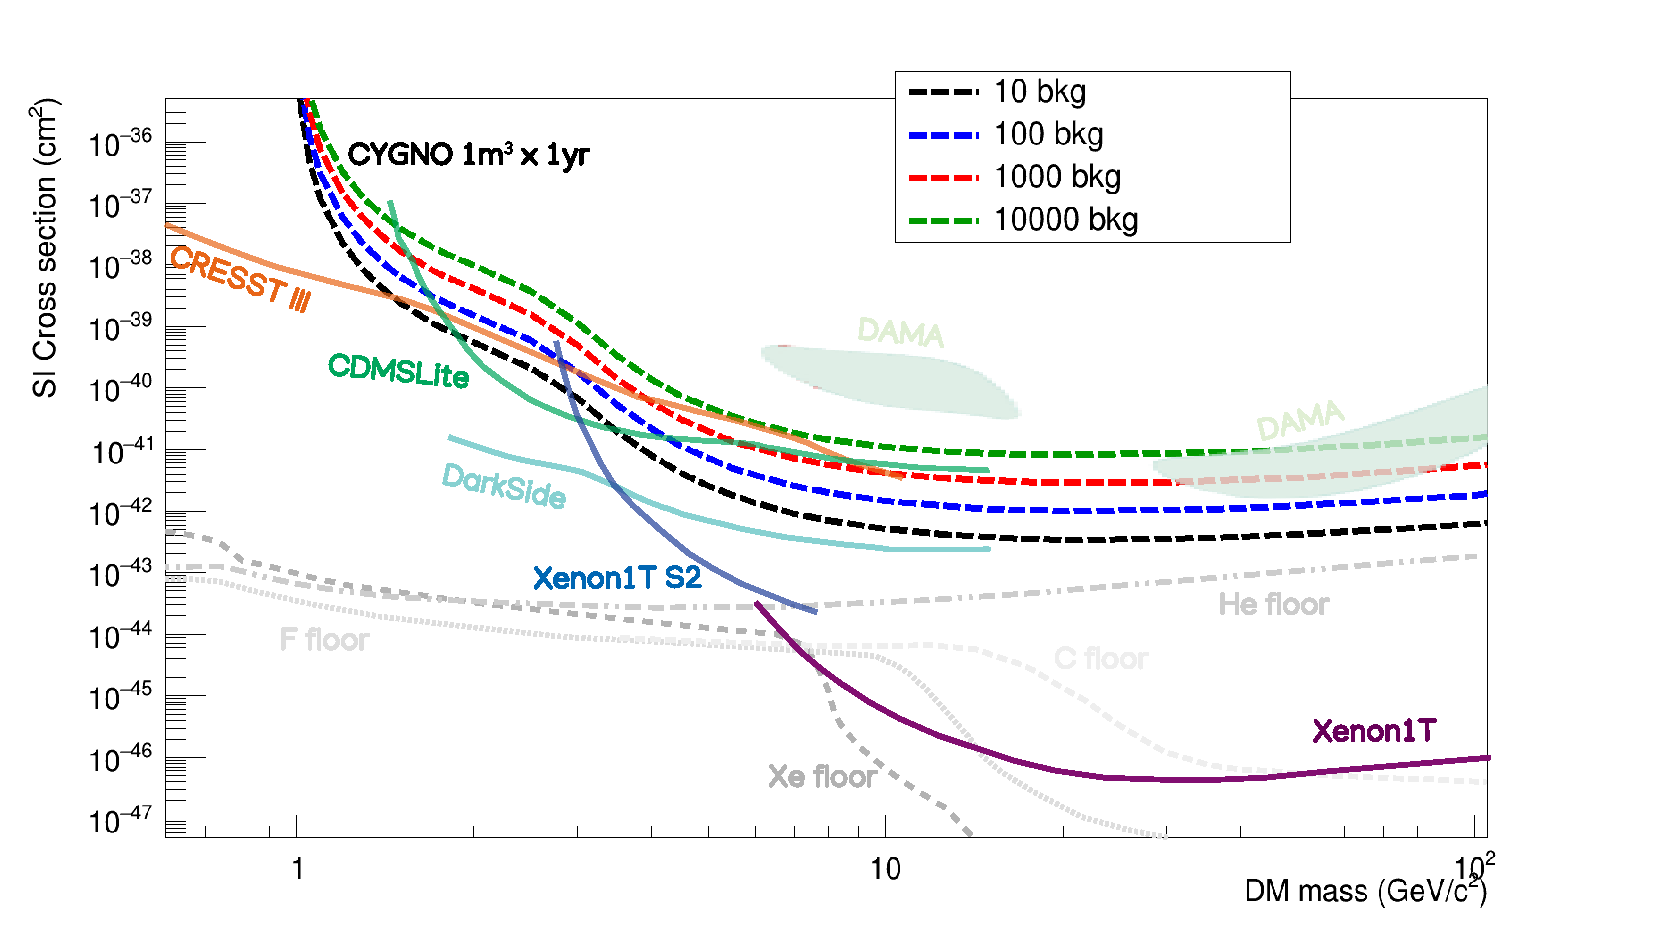
\includegraphics[width=0.7\textwidth]{1m3_1y_4.pdf}
 \caption{\textit{Spin Independent limits for WIMP-nucleon cross section for 1 m$^3$ CYGNO detector for 1 year exposure with different background level assumptions. The line representing other experiment are taken from \cite{bib:Aprile_2018,bib:Aprile_2019,bib:B_hm_2019,bib:Agnes_2018,bib:Agnese_2018,bib:Mancuso:2020gnm,bib:Savage_2009}.}}
 \label{fig:SI}
 \end{figure}
 \begin{figure}[t!]
\centering
 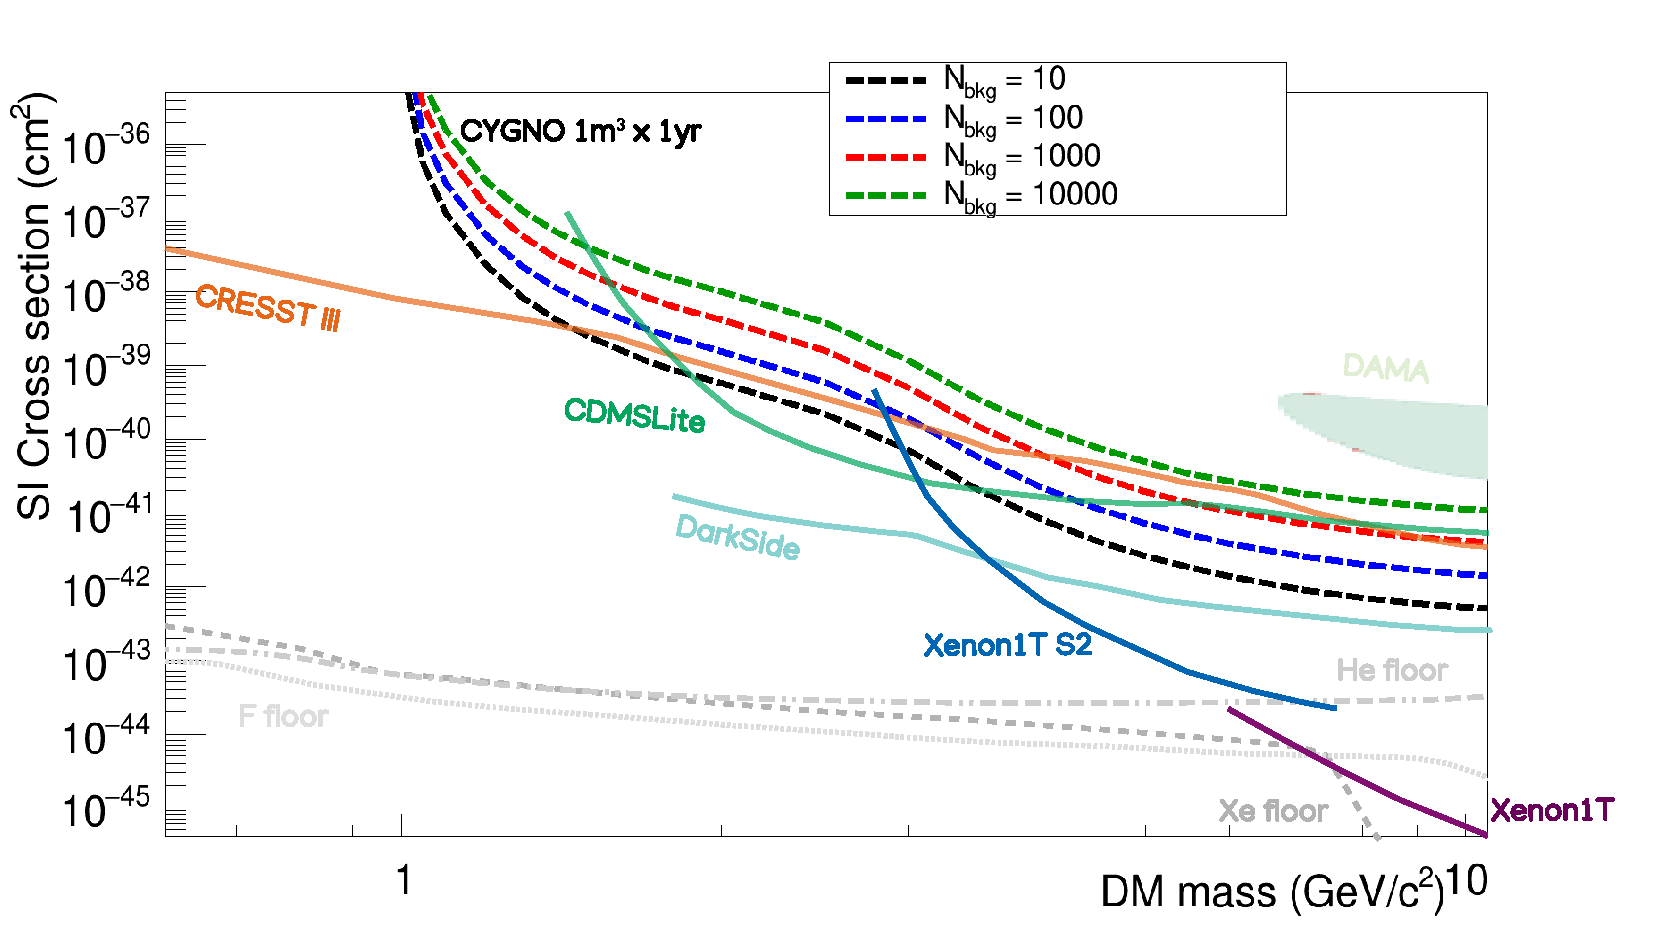
\includegraphics[width=0.7\textwidth]{1m3_1y_4_zoom.pdf}
 \caption{\textit{Spin Independent limits for WIMP-nucleaon cross section for 1 m$^3$ CYGNO detector for 1 year exposure with different background level assumptions limited to 10 GeV/c$^2$ DM mass. The line representing other experiment are taken from \cite{bib:Aprile_2018,bib:Aprile_2019,bib:B_hm_2019,bib:Agnes_2018,bib:Agnese_2018,bib:Mancuso:2020gnm,bib:Savage_2009}..}}
 \label{fig:SI_zoom}
 \end{figure}


As it can be seen, the shape of the limit reflects the different nuclear composition of the gas mixture. The lower DM mass detectable corresponds to the one obtainable with 1 keV$_{ee}$ energy threshold and Helium quenching factor. There is a kink on the curve at around 3 GeV/c$^2$, corresponding to the transition from Helium dominated to Fluorine dominated recoils. The Carbon percentage on the total gas mixture (8\%) is too low to produce a visible effect on the curve. Remarkably, both DAMA regions in the Spin Independent coupling are expected to be accessible by a 1 m$^3$ CYGNO detector for 1 year exposure, making this the first directional detector sensitive to that phase space region.\\
Thanks to the high Flourine content, CYGNO results significantly sensitive also to SD couplings, making PHASE-1 already a relevant competitor in this field, reaching performances comparable to PICO \cite{bib:Amole_2019}, as shown in Fig.~\ref{fig:SD}. 
%It is also important to note that CYGNO is expected to perform much better than its directional competitors such as DRIFT \cite{bib:Battat_2017} both in terms of exposure and lower energy threshold.\\
\begin{figure}[t!]
\centering
 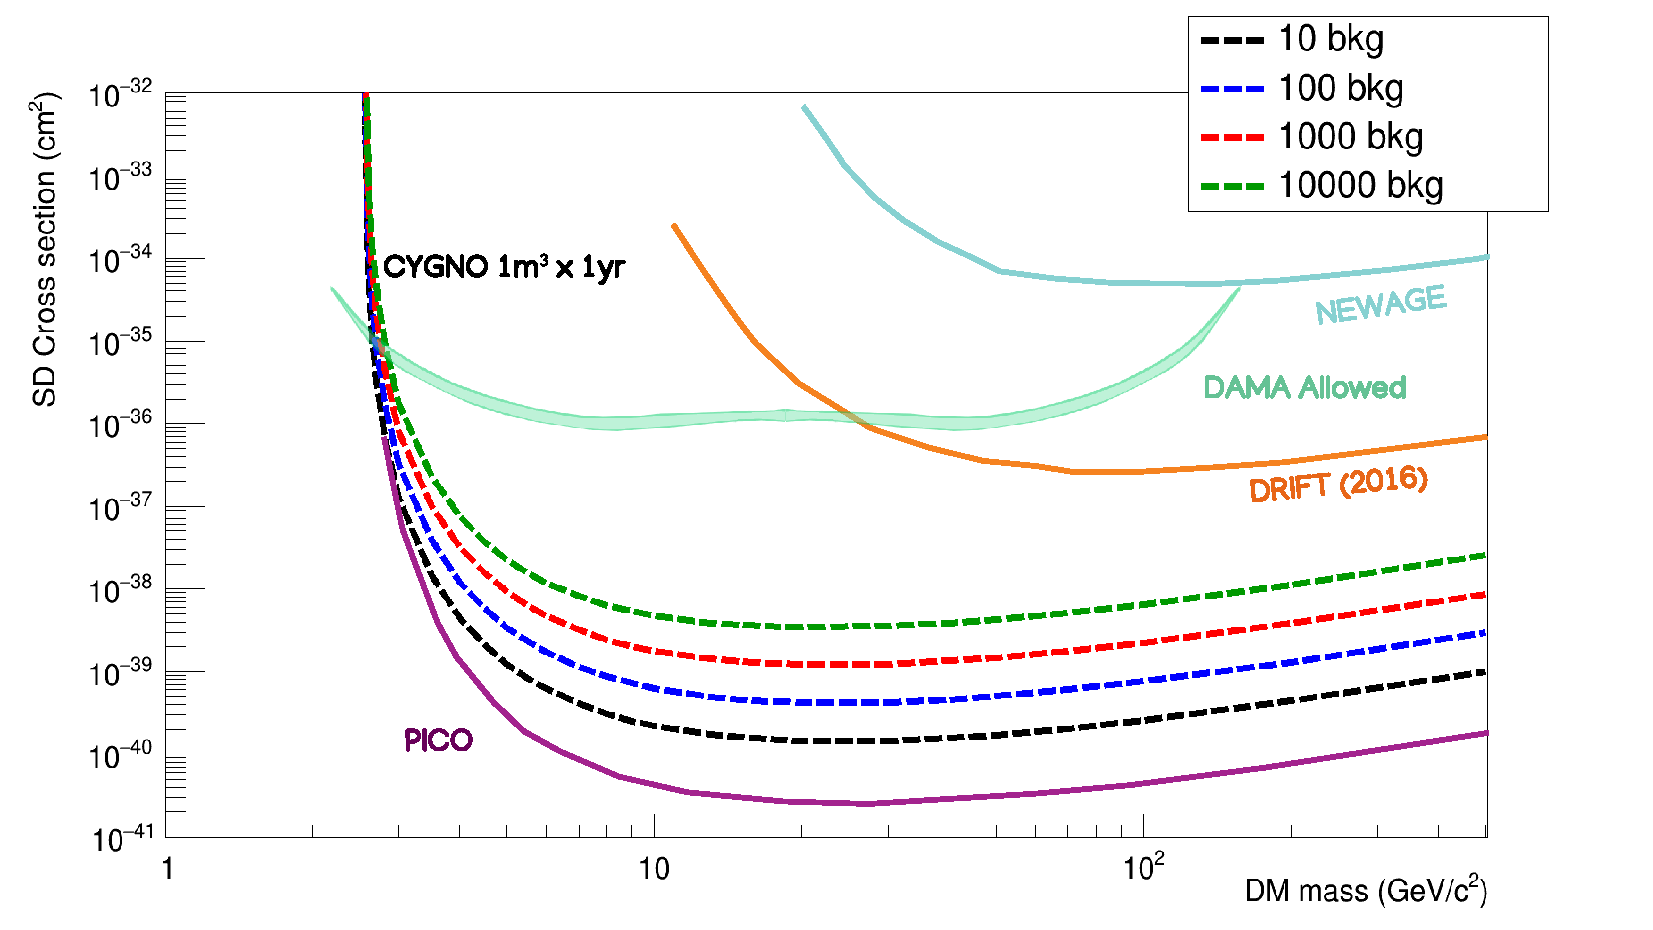
\includegraphics[width=0.7\textwidth]{1m3_1y_SD.pdf}
 \caption{\textit{Spin Dependent limits for WIMP-proton cross section for 1 m$^3$ CYGNO detector for 1 year exposure with different background level assumptions. The line representing other experiment are taken from \cite{bib:Savage_2004,bib:Battat_2017,bib:Amole_2019,bib:yakabe2020limits}.}}
 \label{fig:SD}
 \end{figure}

As a profile likelihood function is used, the shape of the angular distribution will affect the discrimination power. The assumption that directionality is true also at the lowest energies may be a little too optimistic. When comparing CI with a regular likelihood function based on solely the number of events as in Fig.~\ref{fig:nodir}, it turns out that limits decrease by a factor that ranges from 1 to 4. Heavier DM masses, with more spread angular distributions are less affected, than the lighter ones. Also it can be noticed that the larger the number of background events, the stronger the effect of directionality as the lines at 10000 background event are more separated. It is important to note that, though in a loglog scale the outcome of directionality can be barely appreciated, its real strength resides in the potential for positive discovery, other than allowing the discrimination of DM models and DM astronomy after discovery \cite{bib:Baracchini_2020}.
\begin{figure}[t]
\centering
 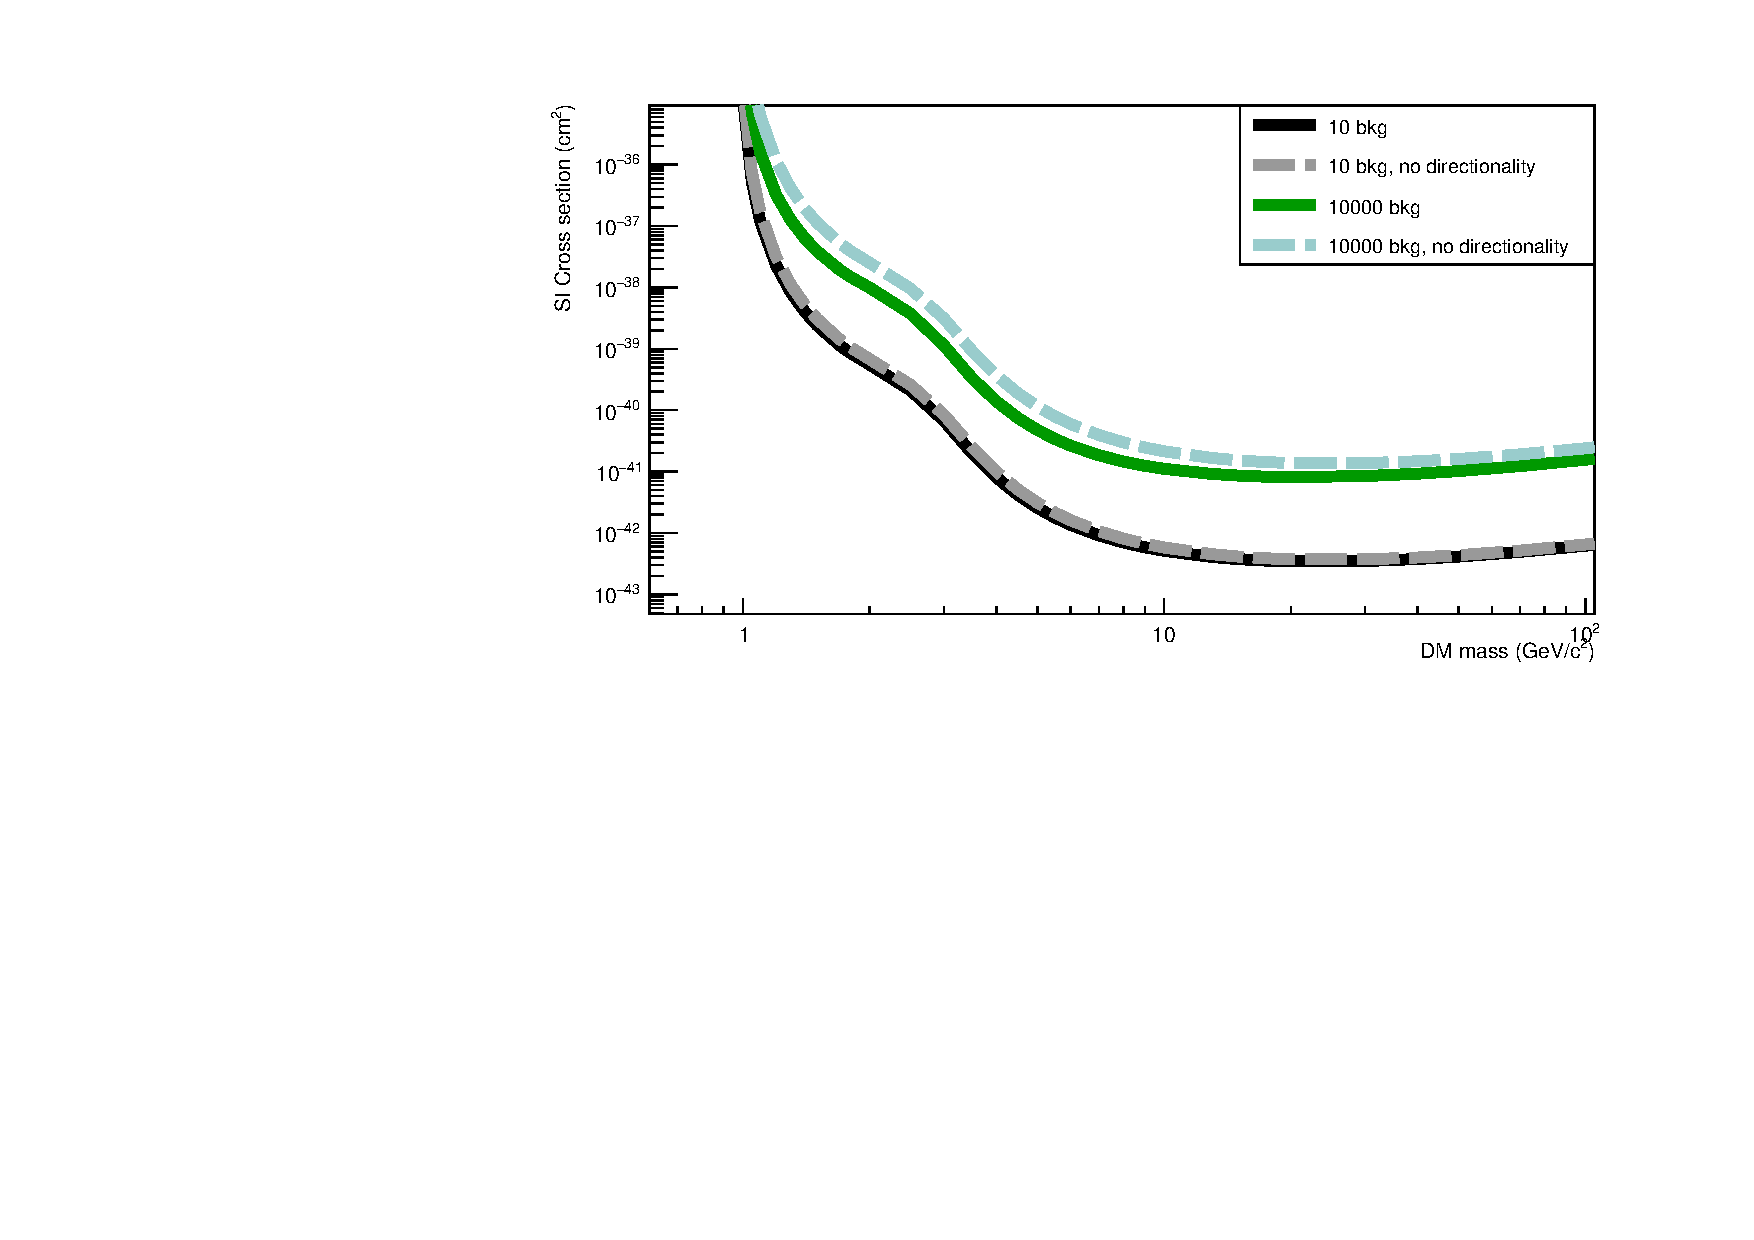
\includegraphics[width=0.7\textwidth]{Compare_directionality.pdf}
 \caption{Comparison of the CI with and without the information of directionality. Two background configurations are considered with an exposure of 1 m$^3$ x 1 yr.}
 \label{fig:nodir}
 \end{figure}


\subsection{Directional searches for MeV Dark Matter produced by Supernovae through nuclear recoil}
While WIMPs still remains highly motivated DM candidates, they are not the only paradigm that can explain the observed DM presence. Core-collapse supernovae (SN) can reach core temperatures in excess of 30 MeV for O(10) seconds, allowing them to produce vast thermal fluxes of particles with masses O(100) MeV at relativistic speeds~\cite{DeRocco:2019jti}. This makes them an ideal astrophysical source for sub-GeV dark matter. The DM candidate emerging from this scenario considered in \cite{DeRocco:2019jti} are dark fermions, but this is not the only possible realisation of such mechanism. Such particles ends up diffusively trapped near the protoneutron star that forms from the SN core. The dark fermions that do eventually escape are produced with a velocity distribution approximately Maxwell-Boltzmann with semirelativistic velocities ({\it v} $\sim$ 1, to be compared to classical WIMPs with {\it v} $\sim 10^{-3}$  ), exhibiting a roughly order-one spread in velocities. This will results in a time-spreading effect during their propagation to Earth up to 10$^5$ years for an average galactic SN, creating an overlap in time of various SN. Given the high SN concentration in the galactic center, the emission of > 100 SN is expected to be overlapping in a diffuse flux at Earth at any given time. This resembles the diffuse flux of SN neutrinos comprising to the Neutrino Floor at energies > 10 GeV WIMP masses.


Thanks to the large dark fermion momentum, such particles, even being of mass of O(10 MeV), would cause in a detector on Earth a measurable nuclear recoil of O(keV) very hard to distinguish from the one induced by a classic WIMP of the Galactic halo by an experiment measuring only the energy deposited in the active volume. Nonetheless, the expected diffuse flux will be strongly peaked towards the Galactic center, due to the large presence of SN in this region compared to extragalactic sources. Thanks to this high degree of anisotropy, directional detector results in a crucial tool to discriminate MeV SN-produced DM with respect to classical WIMP scenarios. It has in fact recently been shown (with participation of CYGNO collaboration members) that a directional approach with realistic experimental performances could distinguish the two scenarios with few detected signal events, typically between 1 to 2 order of magnitude with respect to the yield needed by a non-directional detector \cite{Baracchini:2020owr}. While this study was performed in the assumption of absence of background in the detect events, a full estimation of CYGNO sensitivity to this DM candidate scenario with the tools discussed developed for the WIMP physics case in Sec.\ref{sec:bayes} is under development.

\subsection{Solar neutrinos detection through both nuclear and electron recoil signature}
Solar neutrinos are well known background to DM searches. They can interact in the active volume of the detector either via elastic scattering on the electrons (producing an electron recoil) or coherent scattering on the nuclei (producing a nuclear recoil). 

Since most of current DM experiments possess ER/NR discrimination, typically only the coherent scattering on nuclei is viewed as an irreducible source background, as is in fact denominated "Neutrino Floor". Directionality has been extensively recognised as the preeminent tool to identify and discriminate NR induced by Solar neutrino from WIMP signal event \cite{Mayet:2016zxu,Vahsen:2020pzb, Billard:2013qya}. While a ton-scale experiment is needed to start detecting these events \cite{Vahsen:2020pzb}, due to the low cross section, new physics in the neutrino sector (described in terms of new mediators between neutrinos and electrons and/or quarks or in terms of non standard effective interactions) can increase the rate at low energies \cite{Boehm:2018sux}. This is particularly true for DM mass below 10 GeV, if a new scalar mediator is assumed, where floor can be raised by several orders of magnitude, making this accessible to CYGNO PHASE-2. 

For what concerns ER induced by neutrino-electron elastic scattering, classical DM experiments measuring only the deposited energy in the detector have no means to discriminate them from ER caused by other sources, and hence treat them as background. Detector exhibiting directional capabilities like CYGNO can actually transform these events into a signal. From the ER direction and the Sun position, the angle between the incoming neutrino and the scattered electron can in fact be inferred, providing an unambiguous signal identification just like with directional WIMP searches. Ton-scale gaseous TPC have already been proposed in the past \cite{Seguinot:1992zu,Arpesella:1996uc} to perform Solar neutrino spectroscopy. The Tetrafluoromethane (CF$_4$) gas foreseen to be combined with He in CYGNO gas mixture due to its nice scintillation properties, appears very attractive in this sense \cite{Arpesella:1996uc}, because it possess a significative electron density (1.05 $\times$ 10$^{21}$ cm$^{-3}$) with a low $z$ nuclei, a feature that maximises the number of targets while minimising the multiple scattering. 

About 1 event/m$^3$ per year is expected in a He/CF$_4$ 60/40 gas mixture at 1 atm for an ER energy threshold of 20 keV coming from the $pp$ chain, making this an extremely interesting physics case for CYGNO PHASE-2 experiment. Due to the larger multiple scattering suffered by low energy electron with respect to nuclei, ER direction determination results more complex than with NR tracks. First results from dedicated algorithm developed within the collaboration, inspired from X-ray polarimetry \cite{Soffitta:2012hx}, shows that 30$^{\circ}$ 2D angular resolution with > 80$\%$ sense recognition from the sCMOS images analysis can be achieved at 20 keV in a 1 m$^3$ detector, improving at higher energies. Figure \ref{fig:neutrino} displays the angular distribution for ER induced by Solar neutrinos for 20 keV and 100 keV energy threshold with a 30$^{\circ}$ $\times$ 30$^{\circ}$ angular resolution. Since background events will be isotropically distributed, this shows how even with the limited angular resolution assumed, directionality provides an extremely effective means for high precision solar neutrino measurement. Moreover, the 20 keV energy threshold assumed for the ER translates in about 80 keV threshold on the incoming neutrino,
%If the expected performances can be met with a O(100) kg exposure detector, the latest results from Borexino measuring down to 160 keV \cite{Agostini:2018uly}, could be surpassed by the CYGNO proposed technique, 
opening a new window of opportunity on the $\emph{pp}$ Sun process down to low energy, unreachable to conventional neutrino detectors\cite{Seguinot:1992zu},


\begin{figure}[t!]
\centering
 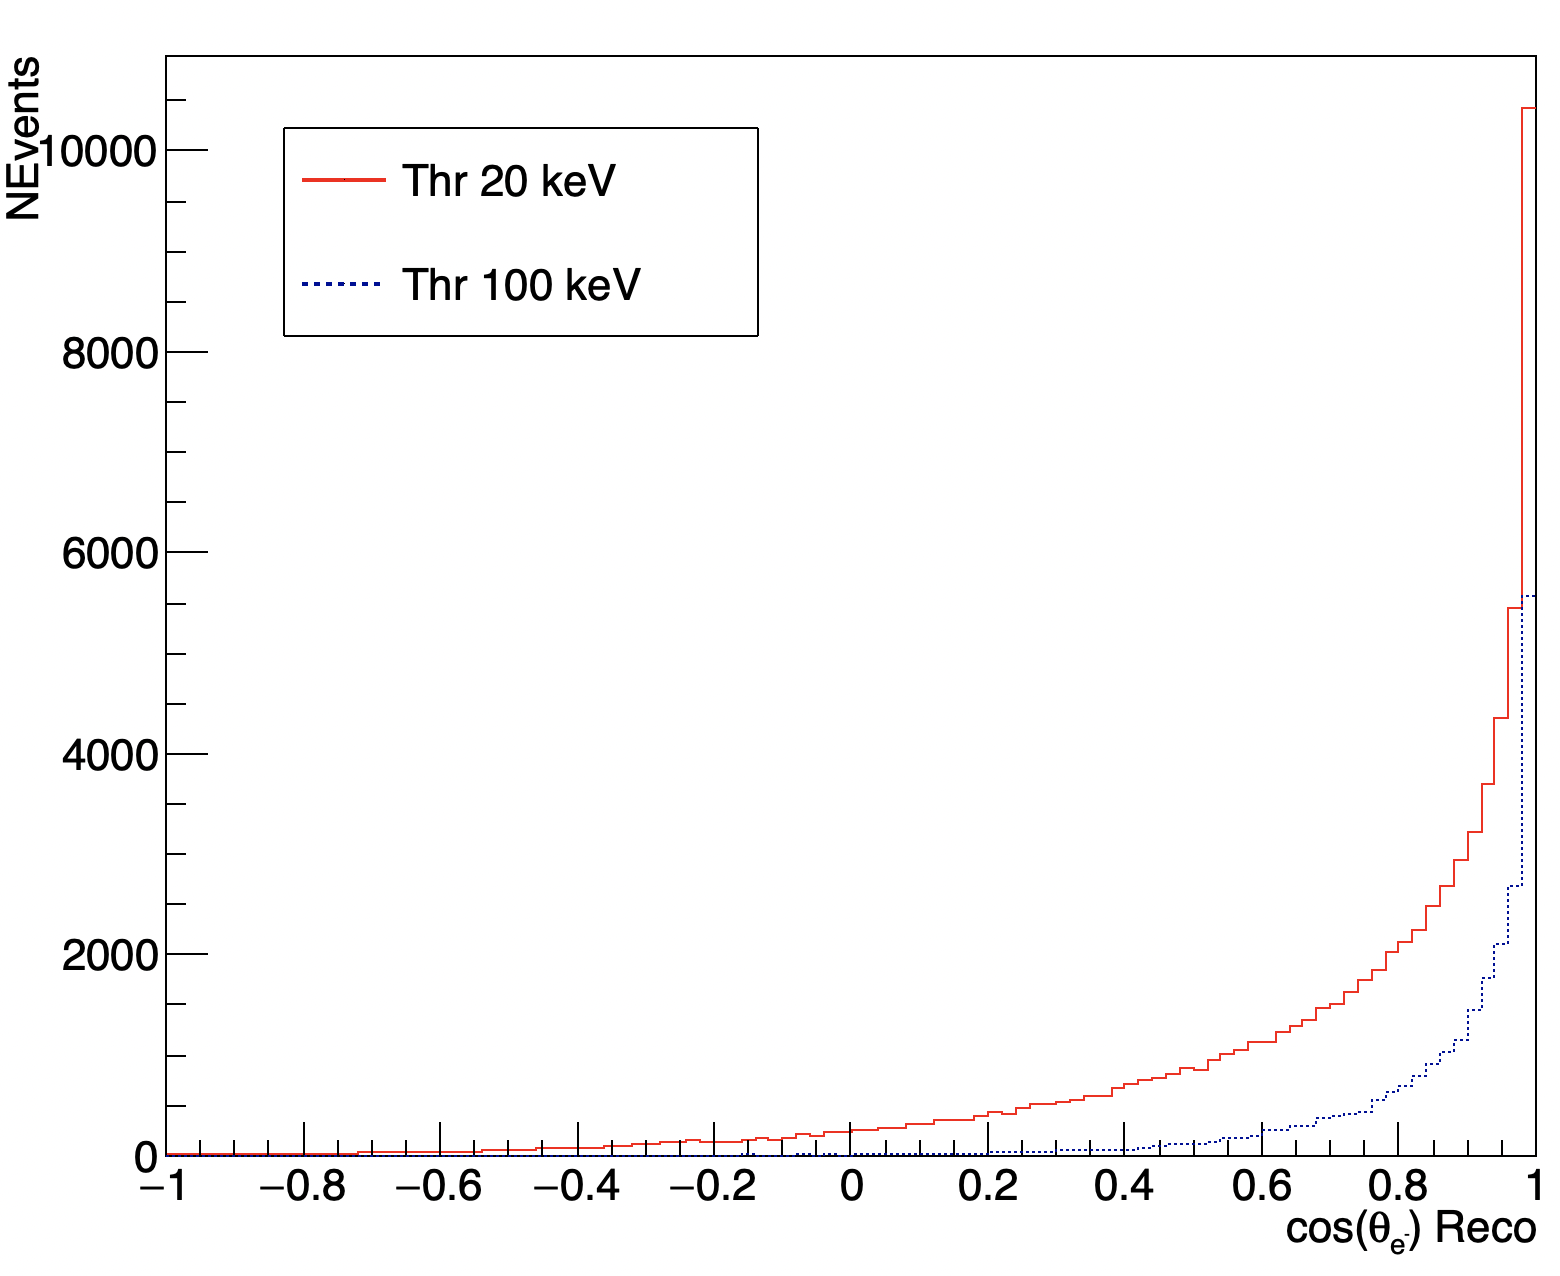
\includegraphics[width=0.35\textwidth]{solar_neutrino_spectrum_20_100_keV.png}
 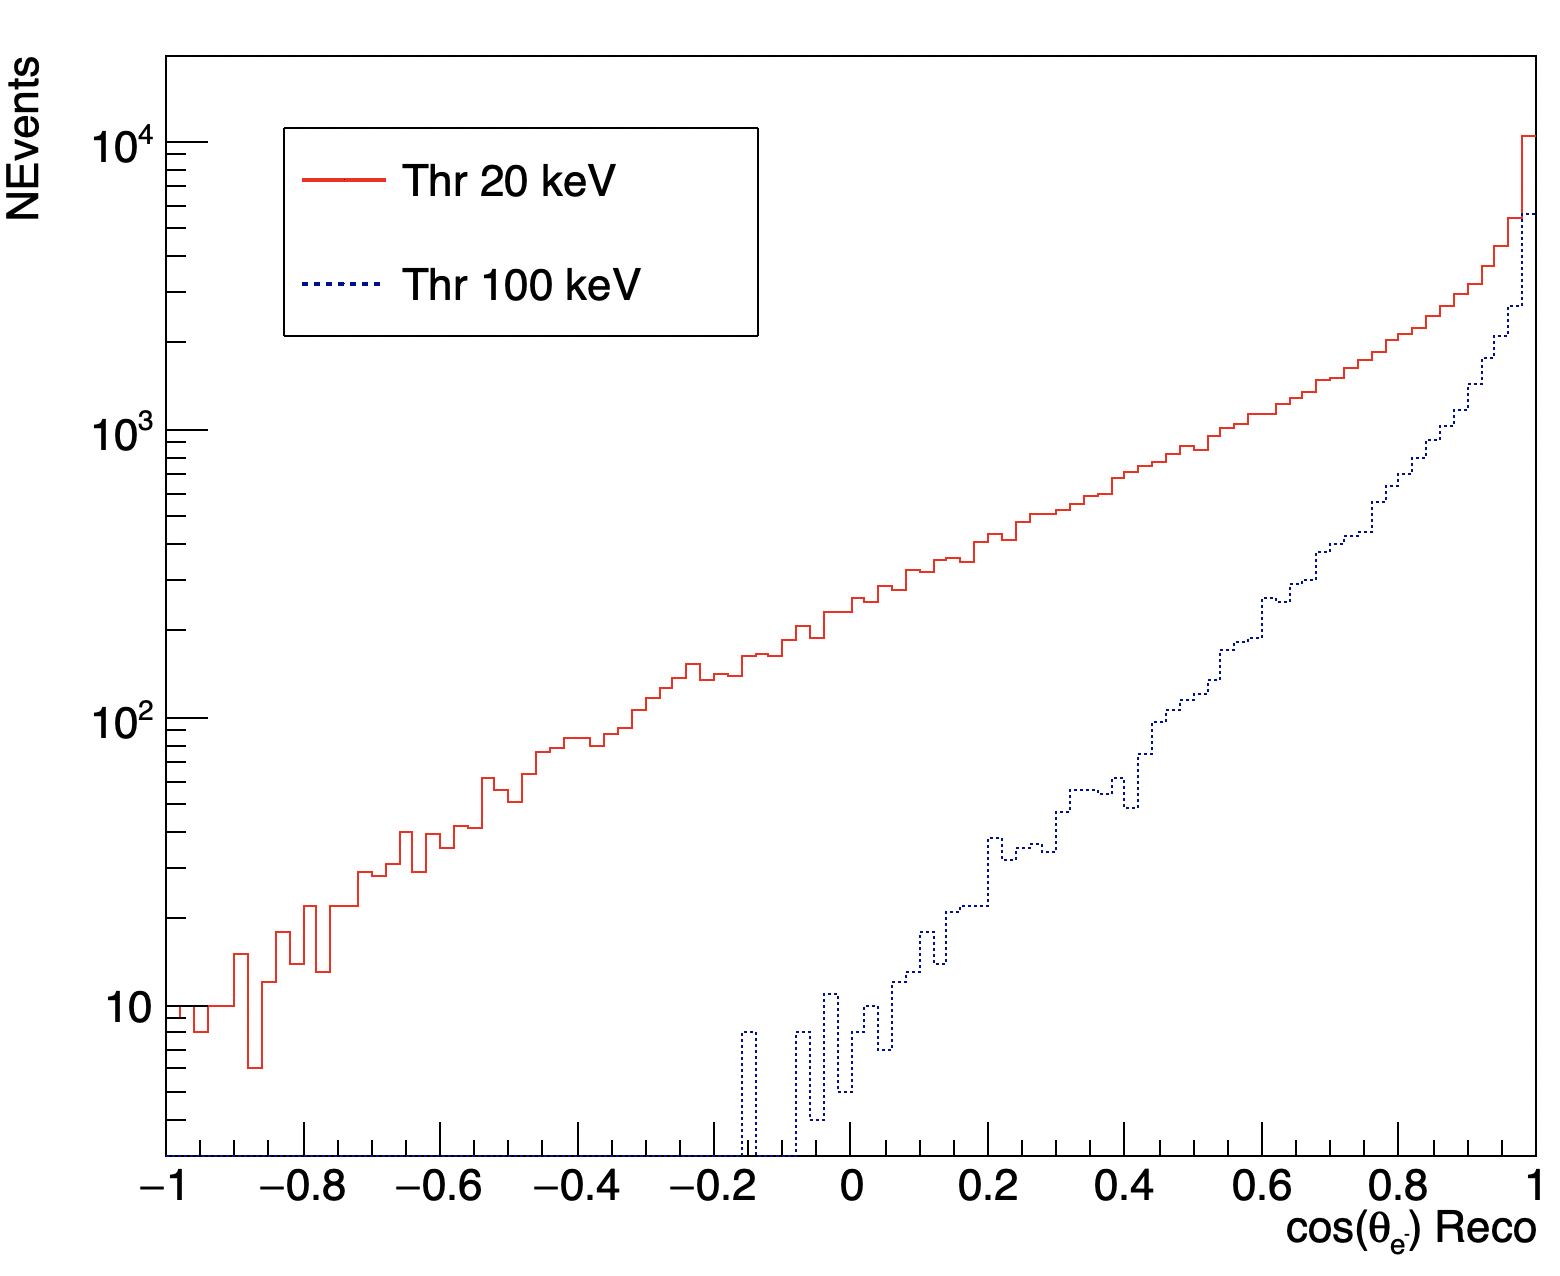
\includegraphics[width=0.35\textwidth]{solar_neutrino_spectrum_20_100_keV_log.png}
 \caption{Angular distribution for electron recoils induced by Solar neutrinos for 20 keV and 100 keV energy threshold with a 30$^{\circ}$ $\times$ 30$^{\circ}$ angular resolution, on the right in log scale.}
 \label{fig:neutrino}
 \end{figure}

%A full physics case sensitivity study is under development within the CYGNO collaboration, and will be the subject of an upcoming paper.


\section{Conclusions}
In this paper, the case for directional DM searches with gaseous TPC with optical readout through the combination of sCMOS images and PMT signals is presented. The performance achieved with a 7~litres prototype based on this approach show the possibility of O(keV$_{nr}$) detection threshold with 10$^2$ ER/NR discrimination at 5.9 keV$_{ee}$.
%obtained with current selection, that can be significantly improved. 
The CYGNO experiment will develop through a staged approach, where the underground installation at LNGS of a 50~litres prototype foreseen for last quarter of 2021 will be followed by a O(1) m$^3$ experiment. From the evaluation of the expected background rate for a 1 m$^3$ detector, properly shielded by Water and Copper, the sensitivity for PHASE\_1 to WIMP searches was evaluated with different background assumptions, reflecting realistic scenarios of performances improvements or underestimation of unexpected contingencies. Additional  physics cases accessible thanks to experiment directional capabilities have been discussed, for which detailed studies are under development.  

The CYGNO approach results therefore highly promising and is expected to be able to significantly contribute to the advancement of TPC technology in the rare event search field.


%no claim for discovery can be made and the data result consistent with a pure background hypothesis, where  WIMP-induced nuclear recoils are considered the signal whilst all the rest is regarded as background.
\newpage
\appendixstart
\appendix
%\begin{appendix}
\section{The Bayesian approach}
The estimation of the expected limits of the CYGNO experiment was performed applying a Bayesian based method. In principle, this approach allows to calculate the probability of any model, given a certain amount of information (data) related to it. This methodology is rarely used in this field, even though it is recently gaining ground \cite{bib:ROSZKOWSKI200910,bib:TROTTA2007316,bib:Strege_2012,bib:arina2014bayesian,bib:Bringmann_2017,bib:Liem_2016,bib:Messina_2020,bib:di_Cortona_2020}.\\
Every model, parameter which is of interest to the specific analysis, and experimental data are all considered connected to a probability distribution and, as such, follow the rules of probability. Exploiting the Bayes' theorem it is possible to find a relation between them and infer a final probability, called posterior, for the desired quantity. In the case of the CYGNO experiment, one is interested in knowing the number of events per year that it will be able to see. Those can be events of background ($\mu_b$) or of signal ($\mu_s$), which is strictly connected to the cross section of WIMP DM particle with protons. The Bayes' theorem can be expressed as follows:
\begin{equation}
\label{eq:Bayes}
 p(\mu,\boldsymbol{\theta}\vert \boldsymbol{D},H) = \frac{p(\boldsymbol{D}\vert\mu,\boldsymbol{\theta},H)\pi(\mu,\boldsymbol{\theta}\vert,H) }{ \int_{\Omega}\int_{0}^{\infty}p(\boldsymbol{D}\vert \mu,\boldsymbol{\theta},H)\pi(\mu,\boldsymbol{\theta}\vert,H)d\mu d\boldsymbol{\theta} } 
\end{equation}

with $p(\boldsymbol{D}\vert\mu_s,\boldsymbol{\theta},H)$ representing the likelihood function $L(\mu_s,\boldsymbol{\theta})$.\\
In equation eq. \ref{eq:Bayes}, the following notation is used:
\begin{itemize}
    \item $p(\mu\vert\boldsymbol{D})$, posterior probability function for the paramenter $\mu$, given $\boldsymbol{D}$.
    \item $\pi(\mu)$, prior probability of a parameter. It includes the expectations of the parameters as well as constrains and knowledge previously obtained from other experiments.
    \item $\mu$, free and of interest parameter representing the expected events due to WIMP-induced recoil ($\mu_s$) or background ($\mu_b$), given a certain WIMP mass (the analysis performs a raster scan).
    \item $\boldsymbol{\theta}$, vector of nuisance parameters, necessary to describe theoretical assumptions and experimental conditions that can affect the results. They can be not completely known and may depend on prior probability distributions. For example, when $\mu=\mu_s$, $\mu_b$, the events expected from the background, becomes a nuisance parameter.
    \item $\boldsymbol{D}$, data set. Can be made of actual experimental data or simulated ones.
    \item $H$, hypothesis under test. It can be the hypothesis of pure background, $H_0$, or the one where both background and signal are present, $H_1$.
    \item $\Omega$, nuisance parameters space.
\end{itemize}

Being in the context of estimating the limits of the CYGNO experiment when data result consistent with a pure background hypothesis, once the posterior probability of the parameter $\mu_s$ is evaluated, it is possible to compute the upper bound as the 90\% Credible Interval (C.I.). This is defined as follows:
\begin{equation}
\label{eq:CI}
 \mu_s(90\% CI): \int_{0}^{\mu_s(90\%CI)} p(\mu_s\vert\boldsymbol{D},H_1)d\mu_s=0.9
\end{equation}
where $p(\mu_s\vert\boldsymbol{D},H_1)$ is the posterior probability marginalised over the nuisance parameters. This value represents the limit under which the true value of $\mu_s$ is, with a 90\% of probability.\\
%\end{appendix}

%\subsubsection{Experimental parameters and assumptions}
%In this subsection a series of considerations will be made regarding the experimental and theoretical inputs and assumptions that were necessary to perform the study.
%\subsubsubsection{Prior probabilities choice}
%Prior probabilities are important elements in the derivation of the posterior ones. In these functions, the current knowledge and expectation of the parameters of interest are present. Obviously depending on them, the final result can turn out to be biased if extreme or wrong assumptions were made. In this work, the only prior probabilities required were the ones regarding $\mu_b$ and $\mu_s$.\\
%About the latter, the actual value of the cross-section of DM with protons is not known and therefore it is difficult to produce articulated priors without risking biases. For this reason, a simple flat distribution between 0 and 1000 was used. Indeed, events per year is a non negative defined variable and due to current limits in the DM community, it is hardly believable that more than 1000 events per year would be produced in the CYGNO detector.\\
%Regarding the prior for the background events, a better estimation can be assessed. The limits produced were performed in the assumption that the background events surviving the discrimination rejection per year were known. As a consequence, the prior was shaped as a poissonian distribution centred on the established background event number. For the future, the simulation of the background together with the discrimination power will provide a single reliable value for the expected background around which to build the poissonian distribution.
%\subsubsubsection{Directionality and Head-Tail recognition}
%Being CYGNO a directional detector, a very strong asset, in order to discriminate events belonging to either WIMP-induced nuclear recoils or background, is the 2D angular distribution of the direction of the tracks. While it is true that CYGNO can measure also the energy of the tracks and that the analysis would profit by combining the energetic and directional information, the core of the enhancement of the discriminating power resides in the directional distribution\cite{bib:Baracchini_2020}. Thus, also for simplicity, the energetic information of the tracks was not be used in this analysis.
%The resulting coordinate space chosen will be the 2D Galactic one. This means that after the occurrence of an event, the direction of the track will be measured and its coordinates will be transformed from the laboratory frame of reference into Galactic coordinates. This way, the available information for the analysis will be not only the number of events, but also their angular distribution in the Galactic frame of reference. This allows the analysis to be based on a profiled likelihood function to exploit the angular distribution.\\
%A relevant aspect that has to be taken into account for the analysis is the angular resolution, which reflects the goodness of the directional information. In principle, it depends on different factors as which particle is recoiling, inclination with respect to the GEM plane and energy of the recoil. Nevertheless, from works of other collaborations on similar setups \textbf{non so chi citare }, the angular resolution is expected to range from 15 up to 30 degrees. Therefore, in order to be conservative the 30x30 degrees squared was chosen for the angular resolution over the whole detectable range.\\
%An equally important parameter is the head-tail recognition, the ability to distinguish the orientation of the track. Preliminary studies show that a head-tail recognition is achievable over 90\%, through energies above 1 keV \textbf{non so chi citare}. As a consequence, a perfect head-tail was considered for energies bigger than 1 keV.
%\subsubsubsection{Angular spectrum}
%In order to compute the profile likelihood function (and to generate fake experiments made of simulated data), it was necessary to predict the angular distribution of both background and signal.\\
%The background angular distribution will be known very well only once it is measured during data taking. It is foreseen to be partially isotropic, coming from the outside the shielding assembly, and partially structured due to presence of internal radioactive material. However, once transformed into Galactic coordinates (taking into account the rotation of the Earth and the motion of the Sun) even these structured components should dilute and the overall distribution will be isotropic at first order.\\
%The signal distributions were calculated in Galactic coordinates, starting from \cite{bib:LEWIN199687,bib:Gondolo_2002,bib:baxter2021recommended}, neglecting the motion of the Earth as it was shown to have secondary relevance on the angular distribution \textbf{da citare }. Possible shapes of the recoil distribution are shown in figure \ref{fig:spectra2D}, where it is clearly visible its anisotropic nature. The final shape of the distribution strongly depends on three elements: the DM mass, the element hit and the energy threshold. With the chosen settings for the analysis, the angular distributions tend to be strongly peaked at low DM masses and more spread at heavier masses, where there is no angular region forbidden by kinematics.
%\begin{figure}[!th]
%  \centering
%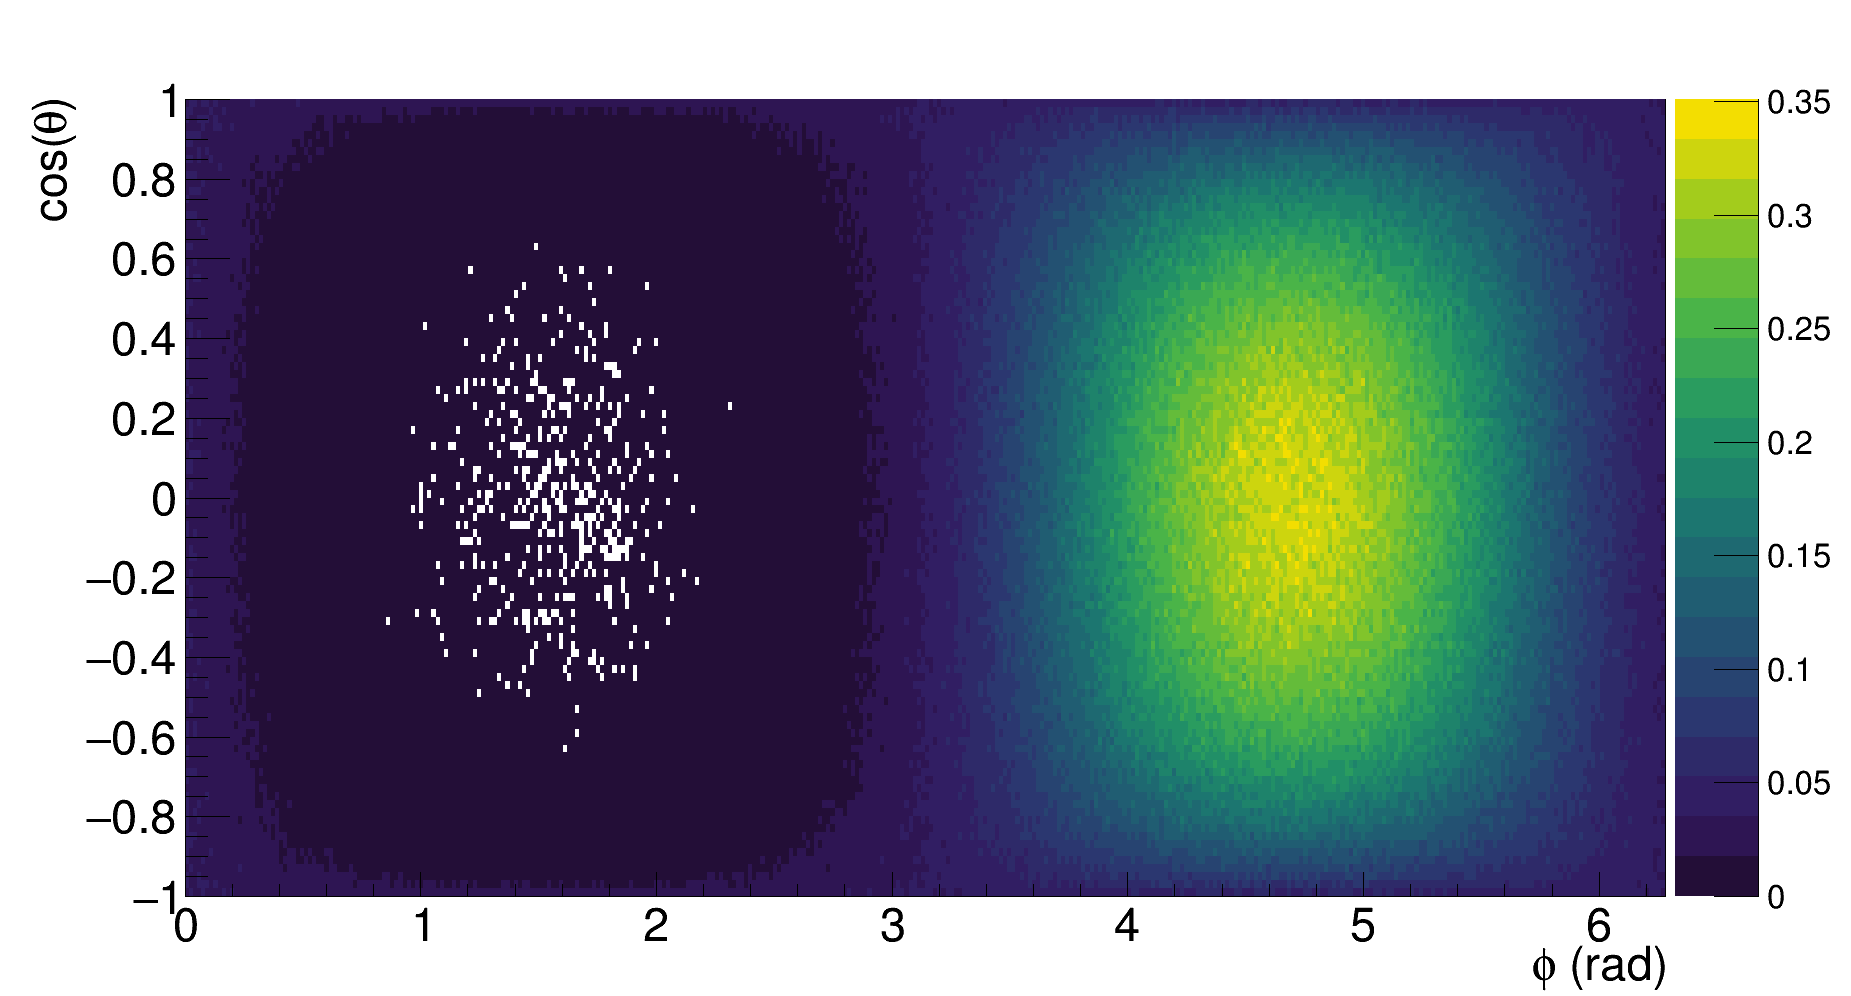
\includegraphics[width=0.35\textwidth]{Heliumrecoil_10GeV.png}
%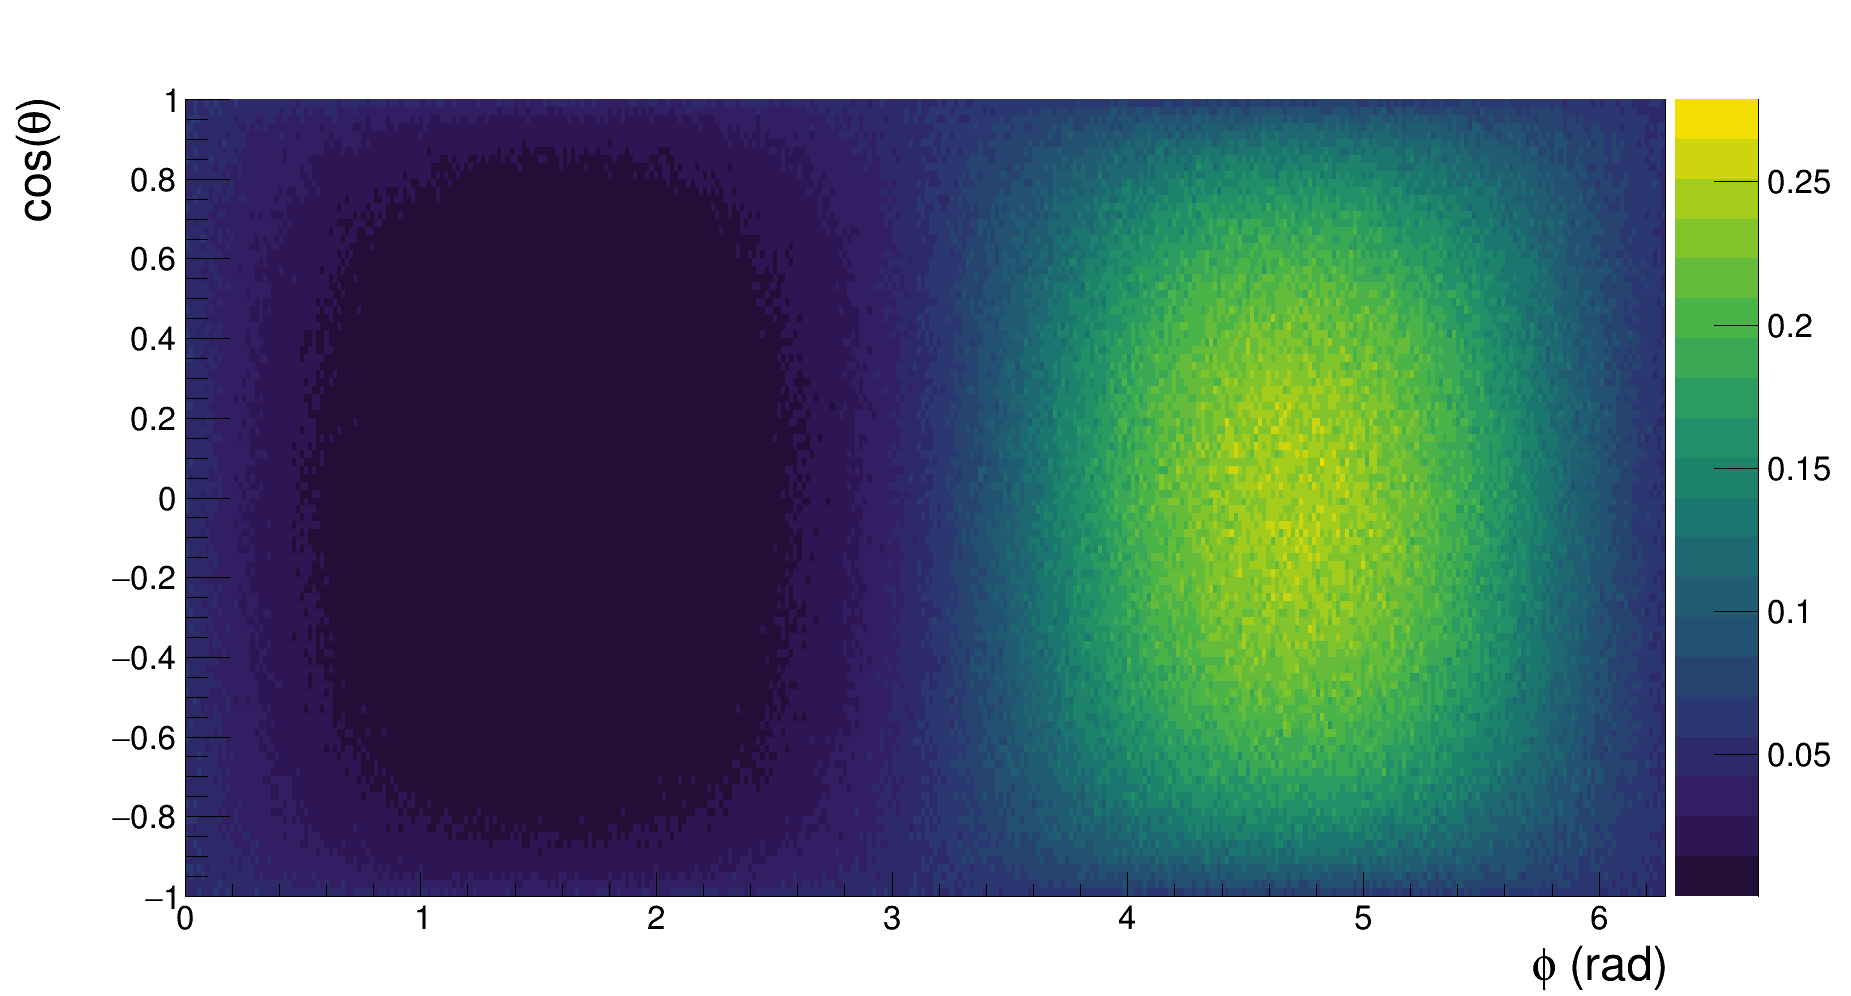
\includegraphics[width=0.35\textwidth]{WIMP_F_100GeV.png}
%\caption{\textit{Two examples of the angular distribution of recoils due to WIMP DM in Galactic coordinates. On the left helium recoils with 10 GeV/c$^2$ DM mass. On the right fluorine recoils with 100 GeV/c$^2$.}}
% \label{fig:spectra2D}
%\end{figure}

%\subsubsubsection{Energy threshold}
%As just stated above, the energy threshold of detection is a key ingredient, not only for the shape of the angular distributions, but also for the limits. Among the astrophysical parameters, the escape velocity, which represents the speed above which any DM particle would have escaped the Galaxy, happens to be  very relevant. Posing a limitation to the speed of DM directly affects the maximum recoil energy of a nucleus. Thus, with an energy threshold larger than that limit, the recoil would be undetectable. Inverting the relation, it means that given an element and an energy threshold, there is a DM mass below which any recoil cannot be detected. Since the gas mixture of the detector is well defined, the shape of the limits will be affected as a consequence. This also helps to understand the reason behind the more peaked distributions at lower DM masses. Indeed, in those conditions only the more energetic recoils, and so with a direction more similar to the incident DM particle, will be detected. The price paid for it, is the limited amount of recoils available, which limits the exposure. Table \ref{tab:Enethreshold} returns a quantitative idea.
%\begin{table}[h!]
%\centering
%\caption{\textit{Lower DM mass detectable for different elements and energy threshold (DM mass in GeV/c$^2$). }}
%\\
%https://docs.google.com/spreadsheets/d/1bgR1mm6i2Z_AnlDX0mlHRTFYeDGw-dXvEvLyFloiAyc/edit#gid=0
%\begin{tabular}{|c|c|c|c|c|} 
% \hline
%\backslashbox{E$_{thr}$ [keV$_{ee}$]}{Element}   %     & Helium   & Carbon         &  Fluorine \\
%\hline
%0.5     &   0.415       &        0.687        &      0.83       \\
%\hline
%1     &     0.615     &          0.996      &     1.23        \\
%\hline
%5     &     1.73     &      2.50          &     3.01        \\
%\hline
%\end{tabular}
%\label{tab:Enethreshold}
%\end{table}


%Published measurements \cite{bib:Antochi_2021} showed the potential of detection of tracks down to 1 keV and hence used in this work as energy threshold.
%\subsubsubsection{Quenching factor}
%As nuclear recoils constitute the signal, the quenching factors have to be taken into consideration. Due to the higher ionization power and the density of the gas, the charge freed by the ions is not the same as if they were electrons. The quenching factor quantifies this difference. Simulations with SRIM package of CYGNO gas mixture were performed to evaluate the quenching factor and are shown in figure \ref{fig:QF}.
%\begin{figure}[H]
%\centering
% 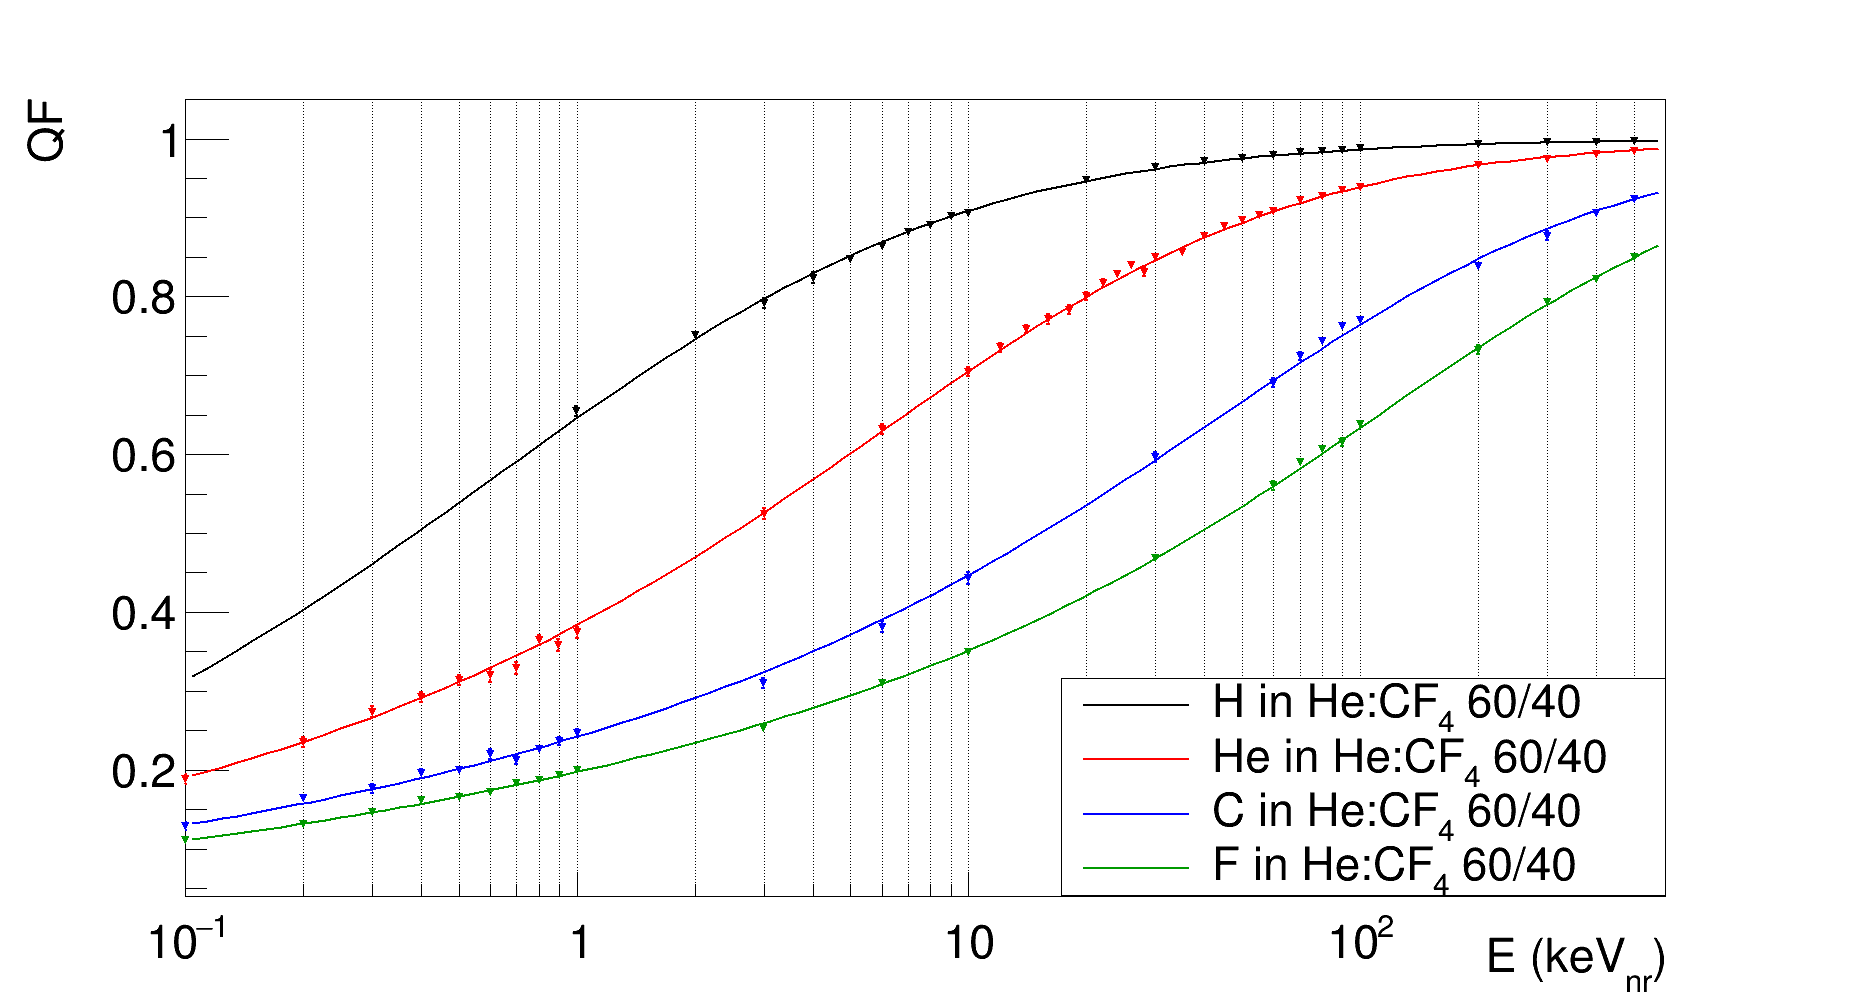
\includegraphics[width=0.7\textwidth]{QF.png}
 %\caption{\textit{Quenching factor values for different elements in a 60/40 He:CF$_4$ as a function of the original recoiling energy.}}
 %\label{fig:QF}
 %\end{figure}
%Practically, when calculating the rates, the quenching factors change the effective energy threshold of detection. As a consequence, 1 keV nuclear recoils cannot be detected and each element, having a diverse ionization power, has a different energy threshold. The limits are affected as a consequence of the modification of the energy threshold. When using 1 keV$_{ee}$ as energy threshold, the effective threshold on the elements becomes 2.14, 3.12, 3.74 keV for helium, carbon and fluorine respectively. 
%\subsubsection{Element probability}
%The gas mixture used comprises three elements: helium, carbon and fluorine. Due to the different percentage of abundance and the kinematics of the scattering, each element nuclear recoil has a different probability of being detected. This was computed by normalizing the rate of each element over the total rate (the cross-section of DM on protons cancels out in this ratios) utilizing the simulated quenching factors and the 1 keV$_{ee}$ energy threshold.
%\begin{figure}[H]
%\centering
% 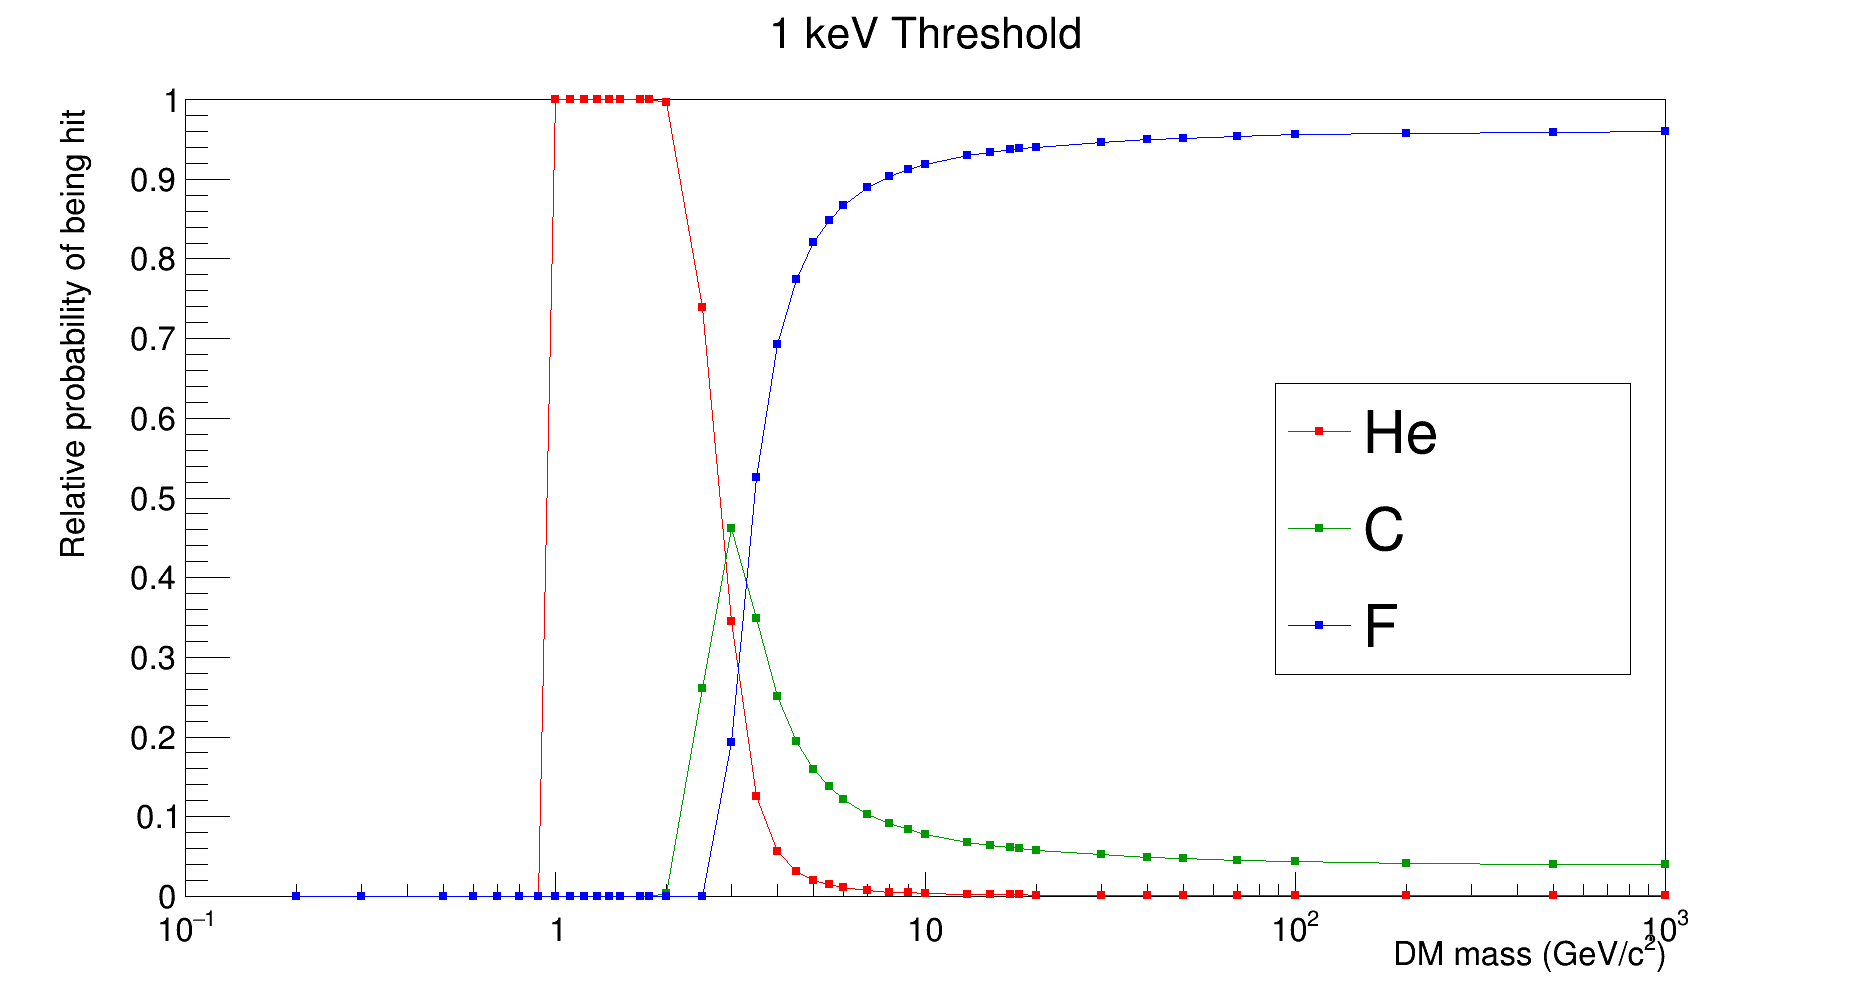
\includegraphics[width=0.7\textwidth]{Prob_hitting.png}
% \caption{\textit{Relative probability of nuclear recoils being detected as a function of the DM mass. The energy threshold is 1 keV$_{ee}$ and the quenching factor corrections are included.}}
% \label{fig:Probele}
% \end{figure}
%The minimum DM mass detectable by each element is clearly visible. Helium recoils dominate the range of low DM masses, while at larger masses, mainly fluorine recoils will happen. 
%\subsubsection{Data simulation and analysis}
%In order to evaluate the CI limits a pool of simulated data was created as the outcome of a fake experiment, taking into account all the elements mentioned above. Once decided the amount of background events (as explained in section (?boh?)), a poissonian random number of background events was extracted and for each of them a direction was assigned, randomly sampling the background angular distribution. After applying a gaussian smearing to account for the resolution, the final direction was filled to histogram in Galactic coordinates, whose binning reflected the angular resolution. As the hypothesis is that no signal was detected, no events for the signal recoils were added.\\

%Once the data sample is prepared, the profile likelihood function is evaluated starting from the following formula:
%\begin{equation}
%\label{eq:likelihood}
% p(\boldsymbol{D}|\mu_s,\mu_b,\boldsymbol{\theta},H_1)=(\mu_b+\mu_s)^{N_{evt}}e^{-(\mu_b+\mu_s)  }\prod_{i=1}^{N_{\text{bins}}} \left[ \left( \frac{\mu_b}{\mu_b+\mu_s}P_{i,b}+ \frac{\mu_s}{\mu_b+\mu_s}P_{i,s}\right)^{n_i}\frac{1}{n_i!}\right]
%\end{equation}
%with:
%\begin{itemize}
%    \item $N_{evt}$, total number of events of the data sample.
%    \item $n_i$, number of events occurring in the i-th bin.
%    \item $P_{i,x}$, Probability of single event to end up in the i-th bin, according to x model (background or signal).
%\end{itemize}
%$P_{i,x}$ includes the probability due to the theoretical angular distribution, to the migration from one bin to another caused by resolution and to which element recoils. The convolution of these is summarised in templates of probabilities, generated for each of the the two hypotheses.\\
%After this step the posterior probabilities can be computed, and $\mu_s(90\%CI)$ can be found for each DM mass and later transformed into a DM particle-proton cross section value.

%To avoid the limits to suffer from any underfluctuation of the background (as undersampling), 500 data samples were created and the average result was taken as final value. 
%\subsubsection{Results}
%Applying all the aforementioned assumptions and technique the projected limits of the CYGNO experiment were calculated, supposing a different background levels, from 10 to 10000 events. Figures \ref{fig:SI},\ref{fig:SI_zoom} show the SI limits together with some recent limits set by other experiments in two separate zoom focuses of DM mass.
%\begin{figure}[H]
%\centering
% 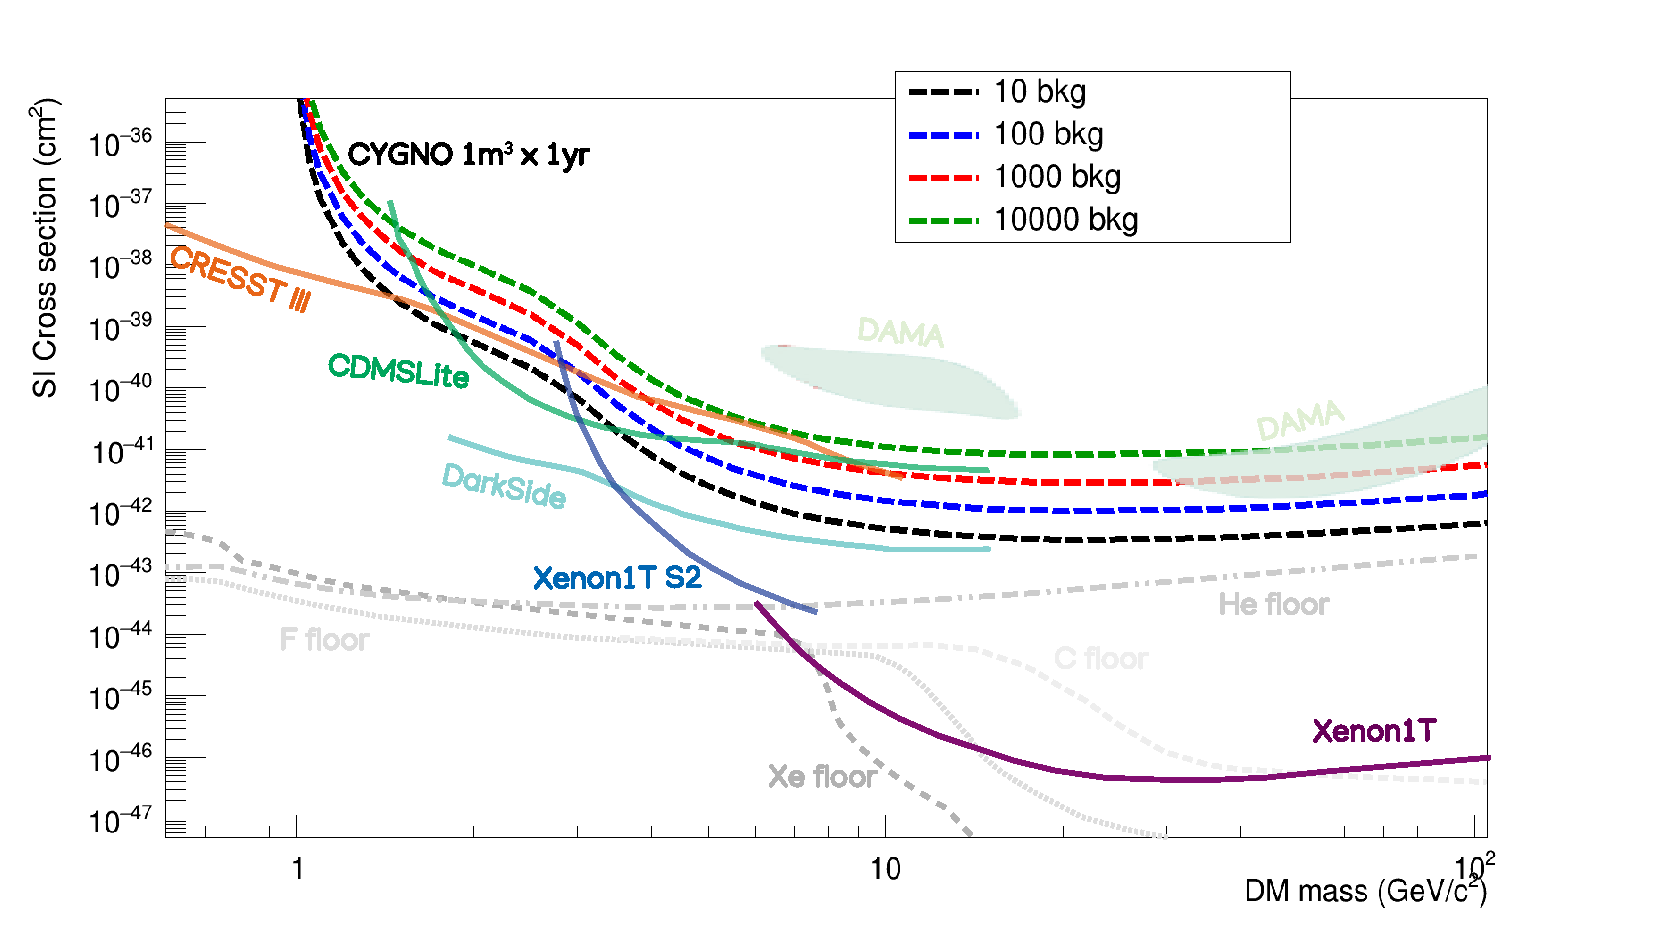
\includegraphics[width=0.7\textwidth]{1m3_1y_4.pdf}
% \caption{\textit{SI limits with different background level assumptions. The line representing other experiment are taken from \cite{bib:Aprile_2018,bib:Aprile_2019,bib:B_hm_2019}\textbf{Darkside cresst dama cdmslite}. Exposure reported on the figure.}}
% \label{fig:SI}
% \end{figure}
% \begin{figure}[H]
%\centering
% 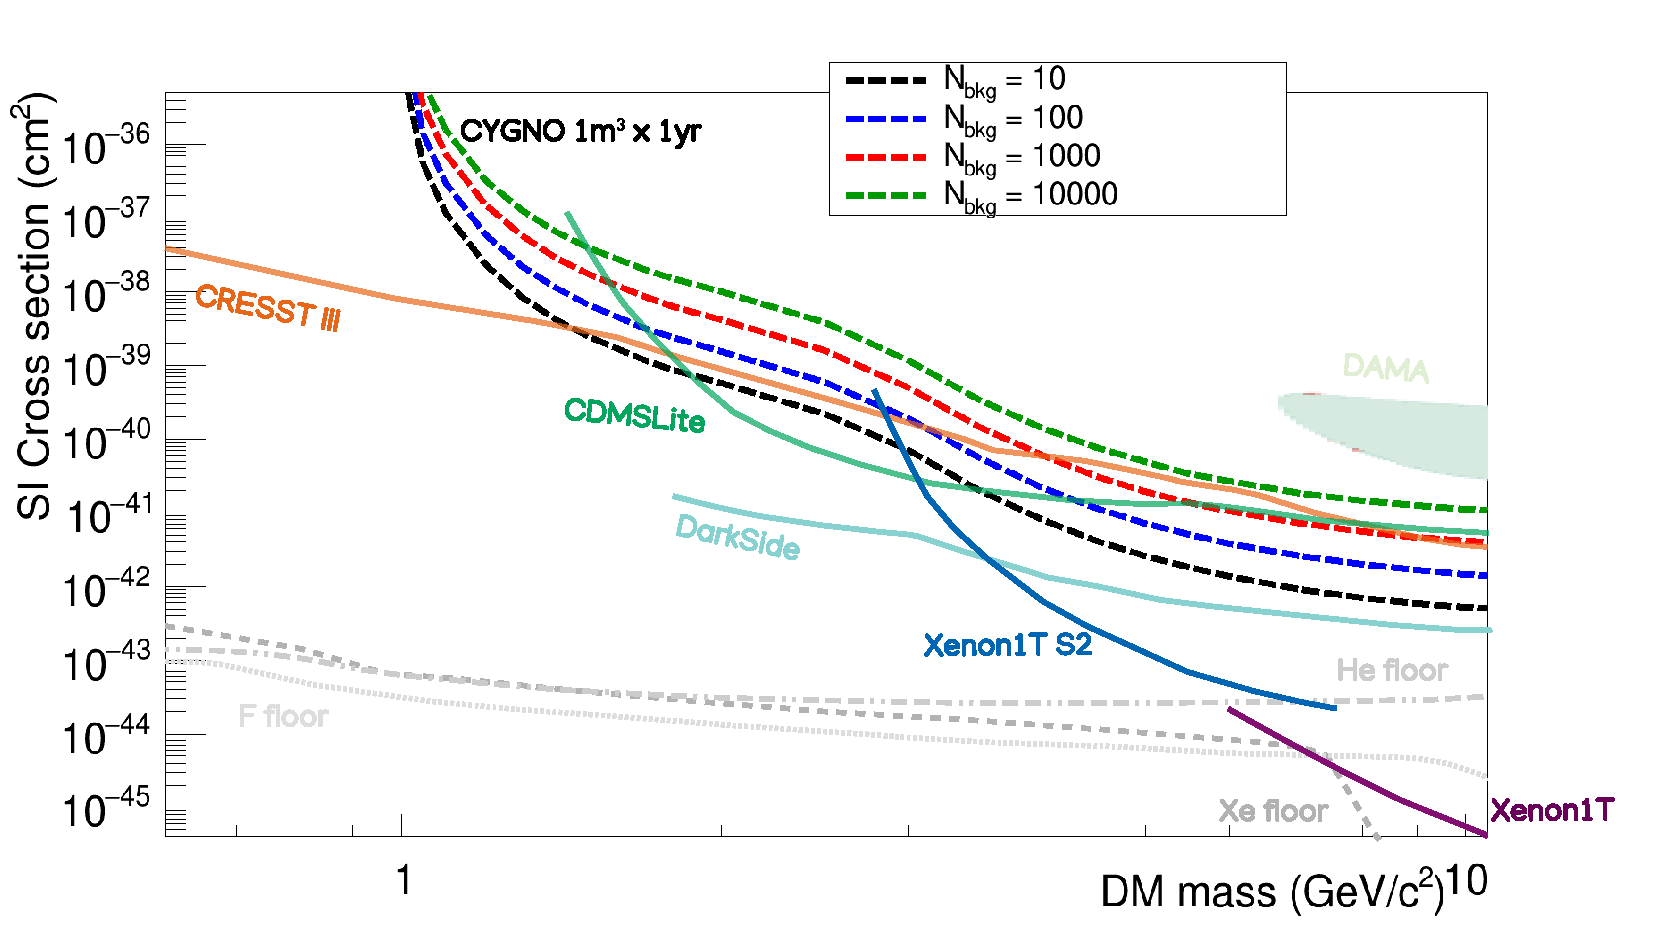
\includegraphics[width=0.7\textwidth]{1m3_1y_4_zoom.pdf}
% \caption{\textit{SI limits with different background level assumptions limited to 10 GeV/c$^2$ DM mass. The line representing other experiment are taken from \cite{bib:Aprile_2018,bib:Aprile_2019,bib:B_hm_2019}\textbf{Darkside cresst dama cdmslite}. Exposure reported on the figure.}}
% \label{fig:SI_zoom}
% \end{figure}


%As can be seen, the shape of the limit reflects the different nuclear composition of the gas mixture. The lower DM mass detectable corresponds to the one obtainable with 1 keV$_{ee}$ energy threshold and helium quenching factor. There is a kink on the curve at around 3 GeV/c$^2$, corresponding to the transition from helium dominated to fluorine dominated recoils. The carbon percentage on the total gas mixture (8\%) is too scarse to produce a visible effect on the curve. Remarkably, both DAMA regions are well accessible by the CYGNO experiment, making it the first directional detector sensitive in that particular area.\\
%As one of the gas constituent is fluorine, also the SD cross section can be scrutinised. The relative high amount of fluorine makes the single cubic meter a relevant competitor in this field, reaching performances comparable to PICO [cita PICO], as shown in figure \ref{fig:SD}. It is also important to note that CYGNO is expected to perform much better than its directional competitors such as DRIFT.\\
%\begin{figure}[H]
%\centering
% 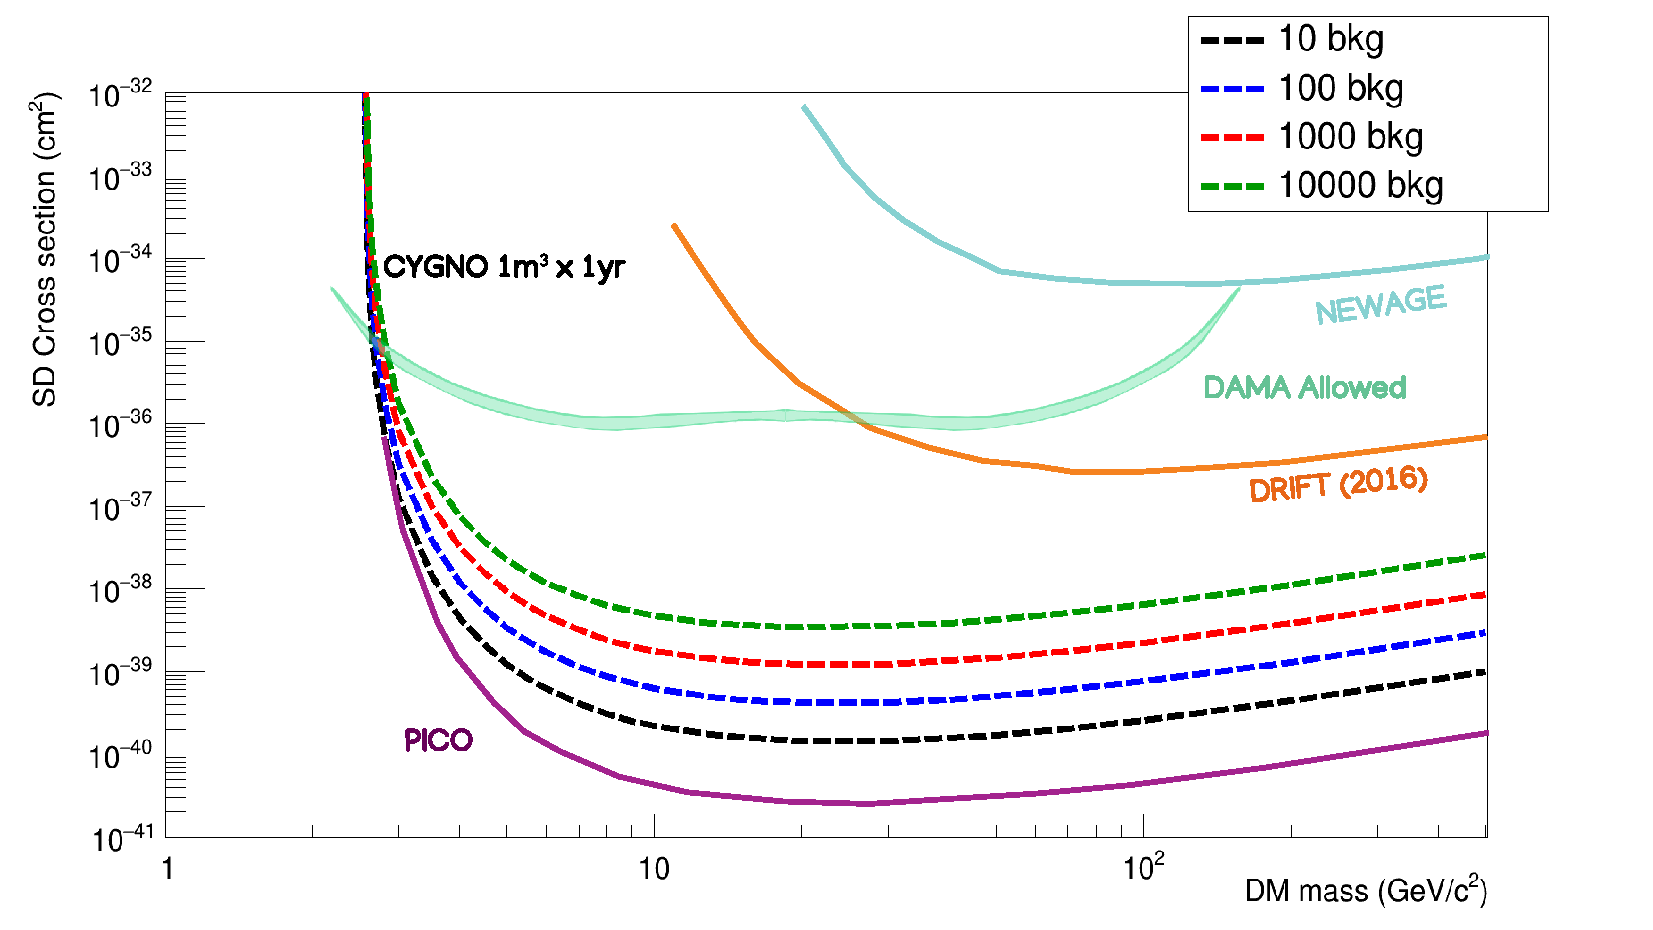
\includegraphics[width=0.7\textwidth]{1m3_1y_SD.pdf}
% \caption{\textit{SI limits with different background level assumptions. The line representing other experiment are taken from \textbf{Drift newage pico}. Exposure reported on the figure.}}
% \label{fig:SD}
% \end{figure}

%As a profile likelihood function is used, the shape of the angular resolution will affect the discrimination power. The assumption that directionality is true also at the lowest energies may be a little too optimistic. When comparing CI with a regular likelihood function based on solely the number of events as in figure[dafare, ho già chiesto a stefano], it turns out that limits decrease by a factor that ranges from 1 to 2. Heavier DM masses, with more spread angular distributions are less affected, than the lighter ones. Also it can be noticed that the more the background events, the stronger the effect of directionality as the lines at 10000 background event are more separated. It is important to note that, though in a loglog scale the outcome of directionality can be barely appreciated, its real strength resides in the potential for positive discovery, other than allowing the discrimination of DM models and DM astronomy after discovery \cite{bib:Baracchini_2020}.


%\subsection{Solar Neutrino Measurement Through Elastic Scattering on Atom Electrons}


\section*{References}

\bibliography{CYGNO-20-001}


\end{document}

